\documentclass{beamer}

%%%%%%%%%%%%%%%%%%%%%%%%%%%%%%%%%%%%%%%%%%%%%%%%%%%% Les packages :
\usetheme{Warsaw}
\beamertemplateshadingbackground{red!10}{blue!10}
\usepackage[english]{babel} 
\usepackage{pgf,pgfarrows,pgfnodes,pgfautomata,pgfheaps,pgfshade}
\usepackage{amsmath,amssymb}
\usepackage[utf8]{inputenc}
\usepackage{textcomp,lmodern}
\usepackage{colortbl}
\usepackage{ucs}
\usepackage{amsmath}
\usepackage{amsfonts}
\usepackage{amssymb}
%\usepackage{natbib}
% \usepackage{media9}
\usepackage{algorithm2e}
\usepackage{multicol}
\columnseprule 0.4pt\raggedcolumns
\usepackage{multirow}
% \usepackage{animate}
\usepackage{tikz}
% \usepackage{multimedia}
\usepackage[natbibapa]{apacite}
\usetikzlibrary{arrows}
\usepackage{pgfpages}
\setbeamertemplate{note page}[plain]

%\setbeameroption{show notes}
%\setbeameroption{show only notes}
%\setbeameroption{hide notes}


%\usepackage{handoutWithNotes}
%\pgfpagesuselayout{3 on 1 with notes}[a4paper,border shrink=5mm]

\beamertemplatetransparentcovereddynamic

%%%%%%%%%%%%%%%%%%%%%%%%%%%%%%%%%%%%%%%%%%%%%%%%%%%% La page de garde :

	\title{Fuzzy Reasoning for Multimedia Semantic Interpretation}
	\subtitle{Fuzzy Ontology Based Model for Video Indexing}
	\author	[\insertframenumber/\inserttotalframenumber \hspace{30mm}  Mohamed Zarka]
		{\textbf{Mohamed Zarka} \\ ~ \\ ~ \\
		{\footnotesize \textit{Advisors:}  \textbf{Prof. Adel M. Alimi} \textit{and} \textbf{Dr. Anis Ben Ammar}}}
	\institute{
		Ph.D. Defense in candidacy for the degree of Doctor of \\ the National Engineering School of Sfax}
	\date{\tiny November $16^{th}$, 2016}

%%%%%%%%%%%%%%%%%%%%%%%%%%%%%%%%%%%%%%%%%%%%%%%%%%%%%

\begin{document}

    	\begin{frame}[plain]
		\begin{tikzpicture}[remember picture,overlay]
    			\node[xshift=-1.5cm,yshift=-7.5cm] at (current page.north east) 
			{
\includegraphics[scale=0.07]{graphics/title/enis.pdf}};
		\end{tikzpicture}
		\begin{tikzpicture}[remember picture,overlay]
    			\node[xshift=1.5cm,yshift=-7.5cm] at (current page.north west) 
			{
\includegraphics[scale=0.08]{graphics/title/regim.pdf}};
		\end{tikzpicture}
      		\titlepage
      	\end{frame}

	\begin{frame}[plain]
  		\frametitle{Outline}
		\setcounter{tocdepth}{1}
		\tableofcontents%[pausesections]
	\end{frame}

	\AtBeginSection[]
	{
		\begin{frame}<beamer>
			\frametitle{Outline}
			\tableofcontents[currentsection]
		\end{frame}
	}

	\section{Introduction}

		\chapter{General Introduction}
\label{intro}
%\addcontentsline{toc}{chapter}{General Introduction}
%\markboth{General Introduction}{}

	\section{Background and Motivation}
	%\addcontentsline{toc}{section}{Background and Motivation}
	%\sectionmark{Background and Motivation}

	Due to the advance of modern multimedia services and techniques, and the exponential growth of online 
	multimedia data, images and video are overflowing our everyday life. \textsc{Flickr}, as a photo 
	sharing website, stores over 5 billion of images and records an uploading rate of over 3000 
	images per minute\footnote{\texttt{http://blog.flickr.net/en/2010/09/19/5000000000}}. 
	\textsc{YouTube} records a rate of 300 hours  of uploaded videos per 
	minute\footnote{\texttt{https://www.youtube.com/yt/press/fr/statistics.html}}.
	Due to this huge amount of available information, and the diversity of their support and content 
	(newscasts, sports, entertainment programs, movies, documentaries, video surveillance, \dots{}), 
	some problems and difficulties are raising, and a need for efficient tools to access to 
	such amount of multimedia content was strongly stated. 

	The common information retrieval model consists in handling useful information through 
	searching and retrieving from large document collections \citep{Baeza-Yates1999,Manning2008,Grossman2012}. 
	Basically, this model is based on two processes: (1) the indexing process which interprets 
	and stores the content of documents, and (2) the search process which matches a user 
	query and the stored document interpretations in order to evaluate their relevance and 
	output relevant documents.
	
	Image and video indexing is basically based on two different approaches: \emph{Text Based} 
	indexing \citep{Chang1980} and \emph{Content Based} indexing \citep{Smeaton2008}. While the \emph{Text Based}
	means that a content is manually annotated by a text describing contained objects and events, 
	the \emph{Content Based} indexing means the extraction of features (like \revAnglais{color} and shape) in order 
	to automatically detect contained semantic objects.


	Authors in \citep{Hauptmann2007,Wang2008,Hauptmann2007a,Kompatsiaris2008,Darwish2015,Ves2015} 
	pointed out that although the availability of many solutions to fill the so-called \emph{semantic gap} \citep{Hare2006}
	between the automatic interpretation and what human expects from the indexing task; 
	none of them yields satisfactory results:  the problem remains open for further research. 
	In \citep{Smeulders2000}, the \emph{semantic gap} is defined as:

	\begin{mydef}
	\textit{``\dots{} the lack of coincidence between the information that one can extract from the visual 
	data and the interpretation that the same data have for a user in a given situation.''}
	\end{mydef}
	
	As illustrated in figure \ref{introduction_2}, the semantic gap manifests itself as a computational 
	problem for the indexing process.  At the low-level, the raw media refers to an image.%, for our example case. 
	The content-based indexing approaches extract features vectors that represent regions of 
	the image or its whole content. At a higher level, the \emph{objects} are detected through combinations
	of extracted features vectors. \emph{Symbolic labels} may be assigned to these objects (\emph{Crowd} and 
	\emph{Road} for the given example). Nevertheless, such a classical process (based on extracting and 
	combining feature vectors) does not typically capture all the semantics in a given content. In fact, 
	the image context and the relationships between the contained objects contribute to \revAnglais{reach a} high 
	level \revAnglais{of} semantic representation and interpretation of the media content.
	Thus, more than the content analysis is
	requested for a better semantic interpretation: The knowledge structure components showed its capabilities to 
	reach such a higher semantic interpretation. Moreover, the information retrieval \revAnglais{is} more and more supported by
	\revAnglais{knowledge} management processes.

% #, thus, essential in order to give a more understanding of present objects and events, and then, a better interpretation for the content.

	\begin{figure}[ht!]
		\centering
		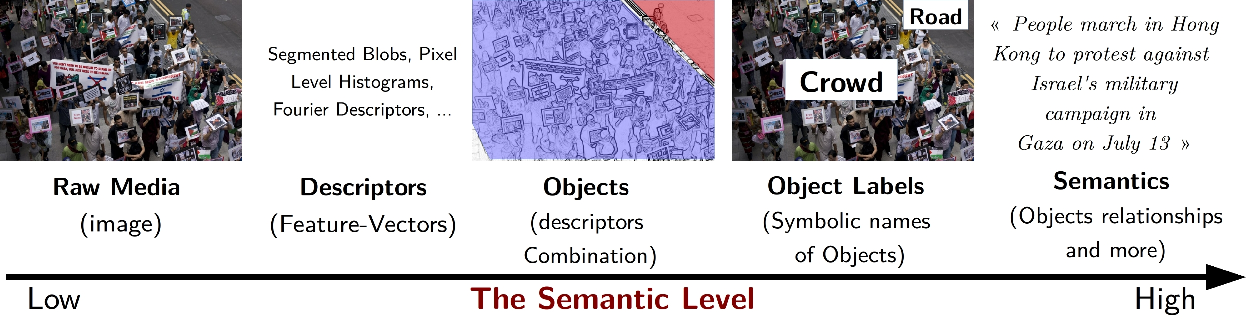
\includegraphics[scale=0.75]{figures/introduction_2.pdf}
		\caption{The Semantic Gap: Hierarchy of levels between the raw media and full semantics}
		\label{introduction_2}
	\end{figure}

	In the current era of multimedia indexing, there is an emerging attention in leveraging massive exploration 
	of knowledge management capacities in order to reduce the semantic gap. Indeed, the use of background 
	knowledge could enrich and enhance  a semantic interpretation about a content. 
	As an example, the figure \ref{introduction_1} displays four images where a classical automatic 
	indexing process could detect the semantic object  \textit{``crowd''} and the semantic object
	\emph{``road''} (for the images $B$, $C$ and $D$). Such a basic object's recognition did not reflect
	the complete semantics of each one.
	
	%Such interpretations of the four images is not enough to properly interpret their contents. 
	%Such a basic object's recognition did not reflect the complete semantics of each one.
	On the other side, the human perception 
	uses a pre-established knowledge in order to better deduce newer information about that content. For the image $A$,
	one can deduce that the \emph{crowd} attends a \emph{Sport Game} (like football). The image $B$ depicts also a 
	\emph{crowd} ahead a \emph{road}, one can deduce also that this \emph{crowd} of people attends a \emph{car racing}. 
	The image $C$ depicts also  a \emph{crowd} ahead a \emph{road}, but one can deduce that  they participate to a protest 
	since people \revAnglais{take} many slogans.  Finally, the image $D$ figures a \emph{crowd} and a \emph{road}, but we 
	can not deduce  nor a \emph{protest} neither a \emph{car racing}; just a \emph{crowd} of people crossing a \emph{road}.

	The aforementioned examples incur a rather weak setting regarding the efficiency of the classical indexing process, 
	establishing the need for a knowledge-based models and approaches. Shedding further light, 
	such a knowledge-based approaches may allow not only for \revAnglais{better semantic interpretation capabilities} but also for 
	the identification of open challenges and future directions and opportunities in multimedia retrieval.

	Through answering many of aforementioned limitations, our motivation goes further toward exploring 
	knowledge-based approaches for enhancing the indexing process capabilities.

	\begin{figure}[ht!]
		\centering
		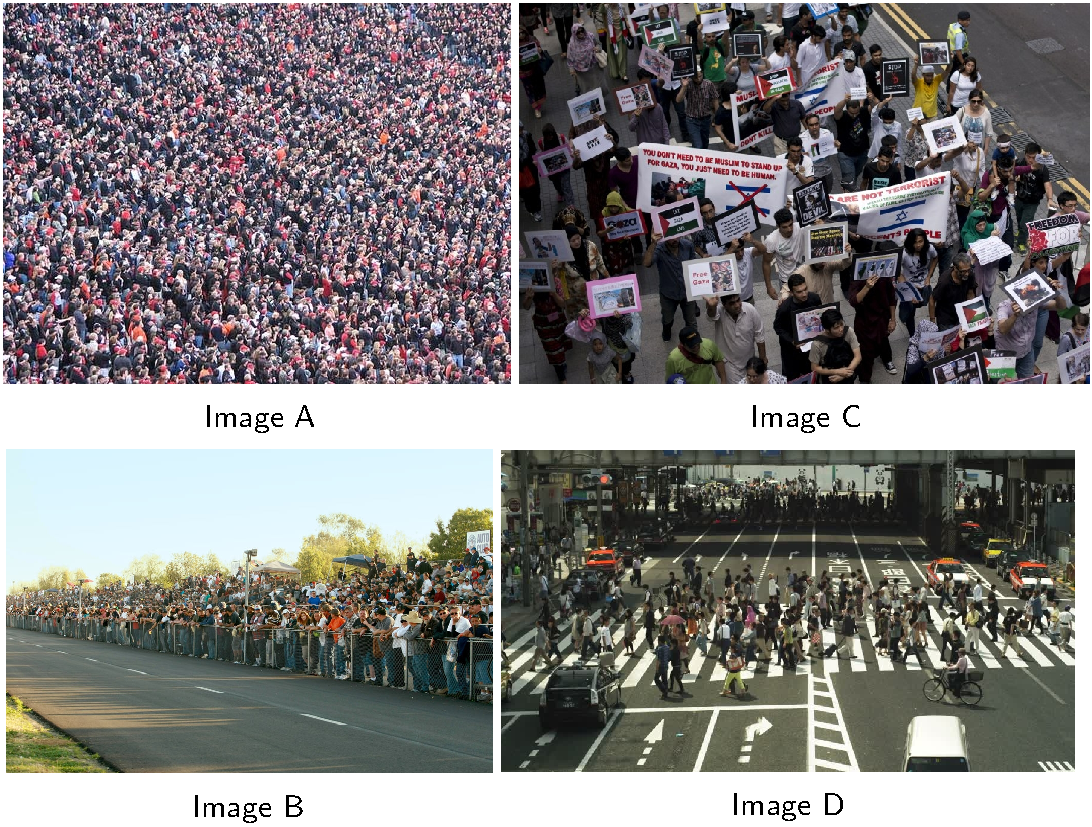
\includegraphics[scale=0.6]{figures/introduction_1.pdf}
		\caption{Different semantic interpretation for images figuring the semantic concept \emph{crowd}}
		\label{introduction_1}
	\end{figure}

	\section{Research Issues}
	%\addcontentsline{toc}{section}{Research Issues}
	%\sectionmark{Research Issues}
	Despite advanced \gls{IR} capabilities, user still unsatisfied by their delivered search results. This discontent 
	is caused commonly by \revAnglais{non-relevant} results that can be due to a \revAnglais{non-good} understanding of stored documents, 
	and/or the \revAnglais{non-apprehension} of the user query. In fact, popular and widely-used search engines, 
	like \textsc{Google}, \textsc{Bing} and \textsc{Yahoo !}, essentially rely on classical 
	keyword matching techniques, and their relevance is often unsatisfying owing to inaccurate 
	textural tag information.

	In such a situation, the multimedia retrieval community has looked for new approaches
	in order to make the availability of automated and efficient semantic interpretations for multimedia contents. 
	Thus, a number of diverse approaches for semantic multimedia content analysis have been proposed addressing 
	the discovery of multi-modal features \citep{Marques2012} like visual features (patterns, color, histograms, \dots{}) and
	audio features. In particular, Content based image retrieval 
	\gls{CBIR} has attracted \revAnglais{a lot of attention} over the last two decades 
	\citep{Rui1999,Smeulders2000,Datta2005,Liu2007,Huurnink2012}. 
	However, these earlier approaches failed to reduce the semantic gap between the extracted features and the 
	user's perception. Then, the next approaches focused on exploring these low-level features in order 
	to detect high level-feature (semantic objects and concepts) \citep{Datta2008,Snoek2008,Egozi2011}. 
	These semantic analysis based approaches proved to be highly effective and useful in many application 
	areas, but, once again, failed to deliver an efficient semantic interpretation \citep{Snoek2010,Over2013}.
	Under such a context, exploring further semantics within a multimedia content is a major challenge.

	To sum up, in our dissertation, we considered that a knowledge based approach should be more explored 
	and tackled. We addressed the following research issues:

	
	\begin{description}
		\item[Issue 1: A novel \revAnglais{knowledge} based approach for video/image indexing]
		other than low-level and high-level ones, further semantic information is gathered 
	from a multimedia content in order to better interpret a semantic content. Motivated by a kindred vision 
	of human perception, new approaches have investigated the engineering of knowledge-based approaches 
	for multimedia retrieval, in particular, the ontologies 
	\citep{Mylonas2008,Hudelot2008,Mylonas2009,Elleuch2011,Paliouras2011,Bannour2014}.
	Yet, ontologies \citep{Petridis2004,Wallace2005,Moeller2008,Dou2015}
	(as a knowledge database) are powerful tools to design concepts/contexts 	
	and their interrelationships. In general, ontology-based approaches 
	\revAnglais{consist} in defining a knowledge conceptualization and a reasoning process in order to handle and 
	enhance a semantic interpretation. However, these recent approaches 
	still facing some issues related to the construction of the ontology and the definition of its content.

		\item[Issue 2: dealing with uncertain knowledge and interpretations]
	Multimedia content interpretation and the user perception give evidence to the uncertain nature of the retrieval
	task which can benefit \revAnglais{from} either fuzzy or probabilistic approaches. In order to model uncertain and 
	imprecise knowledge for multimedia contents, many approaches were proposed. There are many discussions
	about these two approaches and their capabilities to handle and support uncertainty.
	In fact, endless arguments are defended by the knowledge extraction community about  the effectiveness 
	of fuzzy approaches and probabilistic ones \citep{Gaines1978,Bosko1990,Sanjaa2007,Zadeh2014,Zadeh2015}. 
	In this dissertation, we focused on the use of a fuzzy approach. Thus, the use of fuzzy 
	processing techniques to multimedia indexing and retrieval approaches has been extensively investigated 
	in literature. Mainly, fuzzy retrieval models offer more flexibility to handle indexing terms, query 
	terms and pertinent document ranking. The multimedia retrieval community took advantage by the use of 
	fuzzy theory based models for knowledge representation and management.

		\item[Issue 3: Scalability]
	Multimedia collections are increasing staggeringly. Thus, retrieving from large-scale datasets 
	is a challenging task \citep{Villegas2013,Villegas2014,Gilbert2015,Villegas2015}.
	The access to such an enormous \revAnglais{content} has forced the multimedia retrieval community to look for advanced scalable
	approaches and techniques in order to make the availability of automated and efficient semantic 
	annotation for such contents \citep{Wang2011,Zhang2012,Benavent2013,Sahbi2013,Reshma2014}.
	
	\end{description}
	

	Our present thesis work is part of the \textsc{i-Tv} project led by the \textsc{RegimVid} team. 
	The latter project \revAnglais{focuses} on an intelligent and personalized access to a video data system via 
	a complete process from low-level processing to viewing multimedia corpus. Our research works deal 
	with issues of semantic understanding and reasoning for video/image contents. 
	\revAnglais{In the dissertation, we particularly focus on} 
	how to better understand and interpret an uncertain semantic content efficiently through
	the use of fuzzy ontologies. Our approach is based on defining a fuzzy knowledge dataset in order to 
	enhance video/image semantic interpretation, and to overcome the scalability issue. 




%%%%%%%%%%%%%%%%%%%%%%%%%%%%%%%%%%%%%%%%%%%%%%%%%%%%%%%%%%%%%%%%%%%%%%%%%%%%%%%%%%%%%%%%%%%%
	

	\section{Aims and Contributions}
	%\addcontentsline{toc}{section}{Aims and Contributions}
	%\sectionmark{Aims and Contributions}
As aforementioned, the aims of this thesis are threefold. (1) At a first step, we have attempted to suggest a knowledge based model to enhance the indexing accuracy within a multimedia retrieval system. (2) Subsequently, we have concentrated our contributions on an effective use of the knowledge based model in order to improve multimedia content analysis and indexing. (3) Finally, we have concentrated our contributions on the scalability issue when handling large-scale multimedia data and a considerable amount of semantic of their contents.

The figure \ref{introduction_3} illustrates the general work-flow of the proposed approach for a knowledge based framework to enhance the indexing accuracy.


In this dissertation, we attempted to reach the following objectives:

\begin{description}
	\item[Objective 1 ($Obj_{1}$)] Dealing with a new knowledge based model for
		multimedia indexing. The objective is to develop a framework able to handle various information 
		about a multimedia content, then to operate with \revAnglais{this} information in order to infer new 
		information/knowledge through a reasoning process. Such a novel model has to define and highlight 
		pertinent components for an efficient knowledge based indexing process \citep{Zarka2011,Ksentini2012},
	\item[Objective 2 ($Obj_{2}$)] Handling a fuzzy knowledge 
		when reasoning with semantic interpretations in order to enhance and enrich them. This objective 
		aims to define a semantic structure to model required knowledge, then to specify an automated ontology 
		population from available annotated image/video datasets, and finally to handle ontology content evolving 
		to further improve semantics capabilities through \revAnglais{analyzing} and revising inaccurate and irrelevant
		knowledge \citep{Elleuch2011,Zarka2015},
	\item[Objective 3 ($Obj_{3}$)] Ensure the capability to handle a large-scale multimedia indexing 
		collection: the scalability
		While recent works focused on the use of semantic hierarchies to improve concept detector accuracy, 
		this objective embodies the use of such hierarchies to reduce detector complexity and then, to handle 
		efficiently large-scale datasets \citep{Zarka2015a}.
\end{description}


	Consequently, we denote that the outcomes of our thesis work will allow to address the following problems:
	\begin{itemize}
		\item Reducing the semantic gap through providing an effective knowledge based 
			framework for enhancing a semantic interpretation,
		\item Reducing the uncertainty through the use of fuzzy reasoning framework with 
			the aim of assessing the consistency of the indexing process,
		\item Ensuring the scalability aspect through handling hierarchical indexing process 
			which scales well with large-scale multimedia content.
	\end{itemize}

	\begin{figure}
		\centering
		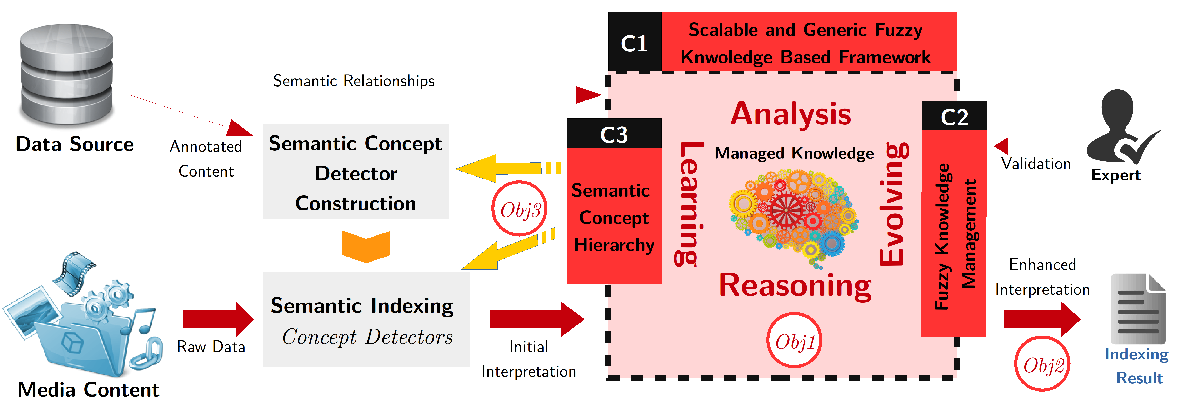
\includegraphics[scale=0.82]{figures/introduction__tmp.pdf}
		\caption{The proposed knowledge based framework: Handle a knowledge dataset to enhance the indexing process accuracy}
		\label{introduction_3}
	\end{figure}

	What was accomplished in our study is a novel ontology management which is intended to a machine-driven
	knowledge database construction. Such a method could enable semantic improvements in large-scale multimedia 
	content analysis and indexing. Thus, the main contributions for our thesis work are enumerated as follows 
	(see figure \ref{introduction_3}):
		\begin{description}
			\item[Contribution 1 ($C_ {1}$):] A fuzzy knowledge based framework for multimedia
				indexing to handle various interpretations about a video content. The framework 
				operates with these initial interpretations in order to infer enhanced interpretations 
				through a fuzzy reasoning process,
			\item[Contribution 2 ($C_ {2}$):] An automated and scalable fuzzy ontology management approach 
				(knowledge extraction, population, reasoning and evolving) for managing and 
				enhancing fuzzy interpretation about a video content,
			\item[Contribution 3 ($C_ {3}$):] A scalable ontology-driven approach to construct hierarchical 
				Semantic concept detectors. Fuzzy knowledge \revAnglais{is} used then at both learning and detection
				steps in order to enhance concept detectors accuracy, and to reduce the number of 
				semantic concepts to be picked up within a content.
		 \end{description}

	In order to illustrate the semantic enhancement of concept detection introduced by our proposed scalable 
	and generic ontology-based framework, the following section enumerates  different conducted experiments 
	within multimedia evaluation campaigns.

%%%%%%%%%%%%%%%%%%%%%%%%%%%%%%%%%%%%%%%%%%%%%%%%%%%%%%%%%%%%%%%%%%%%%%%%%%%%%%%%%%%%%%%%%%%%
	\section{Evaluation and Applications}
	%\addcontentsline{toc}{section}{Evaluation and Applications}
	%\sectionmark{Evaluation and Applications}
	In addition to the theoretical formulation of the proposed approach, we conducted some 
	empirical evaluations over large-scale realistic data sets in the general domains. 
	We first evaluated our approach within the standard benchmark 
	\textsc{\gls{TrecVid}} \citep{Smeaton2006,Smeaton2009,Over2014}. We also applied our 
	approach to real image data from different domains delivered by \textsc{Flickr} data 
	collections \citep{Wang2009}.

	Different evaluation metrics, including \emph{Mean Average Precision} (\gls{MAP})
	\citep{Schoeffmann2012}, \emph{Inferred Average Precision} (\gls{infAP}) \citep{Yilmaz2008} and 
	\emph{Geometric Mean Average Precision} (\gls{GMAP}) \citep{Thomee2012} are used in our experiments. 

	Our evaluations \revAnglais{also concern} the scalability issue. We handled a large scale video 
	dataset (about $8~000$ hours from \textsc{\gls{TrecVid}}) and a large-scale image dataset 
	(up to $500~000$ images from \textsc{Flickr}).

	Based on the proposed approaches and techniques, we participated to the development 
	of the \textsc{RegimVid} system \citep{Elleuch2010,Feki2012,Ksibi2013}:  
	a semantic video indexing, retrieval and visualization system.

	Our conducted experiments can be epitomized within these tasks:
	\begin{itemize}

		\item \textit{Semantic Video Indexing}: We first explored a multi-modal fuzzy fusion model 
		to handle different semantic interpretation gathered by various modalities (text, audio, visual, \dots{}).  
		A practical system was designed to incorporate the latter fusion model. We used the developed system 
		in order to enhance a video semantic indexing within the \emph{Semantic Indexing} task of the 
		\textsc{\gls{TrecVid}} 2010 \citep{Elleuch2010,Zarka2011,Over2011} evaluation campaign,


		\item \textit{Photo Annotation}: After exploring knowledge database capabilities for enhancing 
		a semantic interpretation, we proposed a fuzzy ontology based reasoning framework for managing valuable 
		knowledge in order to open up a semantic interpretation about a content. The proposed framework was 
		evaluated within the \emph{ImageCLEF2012's Flickr Photo Annotation and Retrieval} 
		\citep{Thomee2012,Zarka2015} evaluation campaign,

		\item \textit{Scalable Photo Annotation}: the aforementioned knowledge based framework being formulated 
		and evaluated, we investigated a study on the semantic indexing scalability issue through considering 
		an ontology based hierarchical image annotation. We evaluated, then, this framework within 
		\textit{ImageCLEF2015 Scalable Concept Image Annotation} \citep{Gilbert2015,Villegas2015,Zarka2015a} task.

	\end{itemize}

	\section{Thesis Overview}

	At this point, many questions have arisen: what is an appropriate model/approach to introduce the
	knowledge management in an indexing system? Then, how to profit from a knowledge database to enhance 
	the indexing accuracy? Finally, how to cope with the scalability issue? 

	Keeping in mind our chronological progression in achieving the enumerated above objectives and 
	contributions, the rest of the present dissertation is organized through three parts as follows:

	\begin{enumerate}
		\item \textit{\textbf{Part I - Video Indexing: Background and Trends}}
		\begin{itemize}
			\item \textbf{Chapter \ref{state1}:} introduces a general overview of the Multimedia Information Retrieval.
			It describes also the main proposed models, the common assessment measures and the methodologies.
			The chapter ends with an enumeration of actual video indexing issues and trends.
			
			\item \textbf{Chapter \ref{state2}:} introduces a survey of the use of fuzzy knowledge databases to solve problems 
			discussed in the previous chapter. After enumerating actual related works, we show a discussion 
			over the survey in order to motivate and introduce our proposed fuzzy ontology based model 
			for video indexing	
		\end{itemize}

		\item \textit{\textbf{Part II - Fuzzy Ontology Based Framework for Video Indexing}}
		\begin{itemize}
			\item \textbf{Chapter \ref{c1}:} displays a new approach for video indexing through the use of 
				fuzzy ontologies. Our approach takes advantages of the fuzzy knowledge in order 
				to enhance video indexing accuracy. Then, we focus on modelling and handling \revAnglais{this}
				fuzzy knowledge within an ontology. Therefore, an ontology management model is presented.

			\item \textbf{Chapter \ref{c2}:} proposes to go further in the use of fuzzy ontologies models for 
				enhancing video indexing accuracy. In particular, we address the following issues: 
				how to extract valuable fuzzy knowledge? How to model \revAnglais{this} fuzzy knowledge within
				an ontology? How to reason with \revAnglais{this} fuzzy knowledge in order to improve a semantic
				interpretation? And finally, how to evolve the extracted knowledge? Therefore, we propose 
				to \revAnglais{automatically construct} fuzzy ontologies to handle efficiently information about 
				a video content.

			\item \textbf{Chapter \ref{c3}:} explores the contribution of semantic hierarchies for image annotation 
				in order to handle the scalability issue. Thus, we propose an ontology driven hierarchical 
				image annotation owing to reduce the number \revAnglais{of semantic concepts} to be detected 
				within a content. 
		\end{itemize}

		\item \textit{\textbf{Part III - Conclusions and Future Research Directions}}
		\begin{itemize}
			\item \textbf{Chapter \ref{conlusion}:} states a feedback on our contributions and discusses
				future directions that can be tackled by the presented research topics.
		\end{itemize}
	\end{enumerate}

	

	\section{Publications}
	%\addcontentsline{toc}{section}{Publications}
	The aforementioned contributions in the fuzzy ontology based semantic enhancement for video 	
	indexing have been justified  by the following scientific publications:  
		\paragraph{International Journal}
			\begin{itemize}
				\item \textbf{Zarka, M.}, Ben Ammar, A., \&{} Alimi, A. (2016). 
				Fuzzy reasoning framework to improve semantic video interpretation. 
				\emph{Multimedia Tools and Applications}, $75$(10), 5719–5750. \\Retrieved from 
				\texttt{http://dx.doi.org/10.1007/s11042-015-2537-1}
				\\doi: \texttt{10.1007/s11042-015-2537-1}
			\end{itemize}

		\paragraph{International Peer-Reviewed Communications}
			\begin{itemize}
				\item \textbf{Zarka, M.}, Ammar, A. B., \&{} Alimi, A. M. (2011). 
				Multimodal fuzzy fusion system for semantic video indexing. 
				In \emph{IEEE symposium on computational intelligence for multimedia,
				signal and vision processing, CIMSIVP 2011, Paris, France} (pp. 60--66). IEEE.

				\item Elleuch, N., \textbf{Zarka, M.}, Ammar, A. B., \&{} Alimi, A. M. (2011). 
				A fuzzy ontology: Based framework for reasoning in visual video content analysis 
				and indexing. In Proceedings of the eleventh international 
				workshop on multimedia data mining (pp. 1--8). New York, NY, USA: ACM. \\
				Retrieved from \texttt{http://doi.acm.org/10.1145/2237827.2237828}\\
				doi: \texttt{10.1145/2237827.2237828}

				\item Ksentini, N., \textbf{Zarka, M.}, Ammar, A. B., \&{} Alimi, A. M. (2012). 
				Toward an assisted context based collaborative annotation. In P. Lambert (Ed.), 
				\emph{10th international workshop on content-based multimedia indexing, 
				CBMI 2012, Annecy, France, June 27--29, 2012} (pp. 71--76). IEEE.\\
				Retrieved from \texttt{http://dx.doi.org/10.1109/CBMI.2012.6269852}\\
				doi: \texttt{10.1109/CBMI.2012.6269852}
			\end{itemize}
		\paragraph{International Benchmarks}
			\begin{itemize}
				\item Elleuch, N., \textbf{Zarka, M.}, Feki, I., Ammar, A. B., 
				\&{} Alimi, A. M. (2010). REGIMVID at TRECVID2010: semantic 
				indexing. In P. Over et al. (Eds.), \emph{TRECVID 2010 workshop
				participants notebook papers, Gaithersburg, MD, USA, November 2010}. 
				National Institute of Standards and Technology (NIST). \\
				Retrieved from \\\texttt{http://www-nlpir.nist.gov/projects/tvpubs/tv10.papers/regim.pdf}

				\item \textbf{Zarka, M.}, Ben Ammar, A., \&{} Alimi, A. (2015). 
				Regimvid at imageclef 2015 scalable concept image annotation 
				task: Ontology based hierarchical image annotation. 
				In \emph{Working notes for CLEF 2015 conference , 
				Toulouse, France, September 8--11, 2015.}
			\end{itemize}




%%%%%%%%%%%%%%%%%%%%%%%%%%%%%%%%%%%%%%%%%%%%%%%%%%%%%%%%%%%%%%%%%%%%%%%%%%%%%%%%%%%%%%%%%%%%%%%%%
	\section{Literature Review}
		\subsection{Knowledge-based approaches for multimedia indexing}
\begin{frame}
	\frametitle{Knowledge-based approaches for multimedia indexing I}
	\begin{itemize}
		\item \textbf{Knowledge-based approaches}
		\begin{itemize}
			\item Dealing with semantic \alert{concepts co-occurrence} 
			      \\ {\tiny{\citep{Feng2012,Zheng2013}}}
			\item Dealing with semantic \alert{contexts} 
			      \\ {\tiny{\citep{Dumitrescu2009,PerpetualCoutinho2012}}}
		\end{itemize}
		\item \textbf{knowledge management} (like ontology) are being used in order to handle knowledge  
			about \alert{semantic concepts}, \alert{contexts} and their \alert{relationships}:
			{\tiny{\citep{Noy2001}}}
			\begin{itemize}
				\item knowledge semantic structure
				\item knowledge mining and population (\alert{abduction})
				\item knowledge inferring (\alert{deduction})
				\item knowledge evolving
			\end{itemize}
	\end{itemize}
\end{frame}

\begin{frame}
	\frametitle{Knowledge-based approaches for multimedia indexing II}
	
		\begin{itemize}
			\item \textbf{Related Works}
				\begin{itemize}
					\item \alert{Lightweight Ontologies}: modeled as direct graphs in which nodes  
					represent semantic concepts %{\tiny{\citep{Fan2008,Li2010}}}%,Reimer2012}}} 
					(\textsc{LsCom} {\tiny{\citep{Kennedy2006}}})
					
					\item \alert{Formal Ontologies}: based on \textbf{description language} 
					\\{\tiny{\citep{Mylonas2009,Simou2008,Bannour2014}}}
						\begin{itemize}
						
							\item $\mathcal{T}$ (TBox) a set of \textit{concept axioms} 
										and \textit{role axioms}
		
								\alert{\textit{ex.}} \textbf{Object} and \textbf{Multimedia Content}
								are two ontological concepts under $\mathcal{T}$,
								
								\textbf{\textit{isIndexedBy}(Multimedia Content,Object)} a role that 
								denotes a particular relationship.
							%\pause
							\item $\mathcal{A}$ (ABox) a set of \textit{assertional axioms}
								\\ \alert{\textit{ex.}} \textbf{\textit{isIndexedBy}(Video.mp4, Airplane)}
						\end{itemize}
				\end{itemize}
		\end{itemize}
		\pause
		\begin{alertblock}{}
			\alert{The abduction is still manual: contexts and concept inter-relationships are 
				defined by experts}
		\end{alertblock}
\end{frame}

% \begin{frame}
% 	\frametitle{Knwoledge-based approaches for multimedia indexing III}
% 		\textbf{Related Works}
% 		\begin{itemize}
% 			\item \textbf{Light ontologies}
% % % 				\begin{itemize}
% 					\item \textsc{LsCom}
% 				\end{itemize}
% 			\item \textbf{Formal ontologies}
% 				\begin{itemize}
% 					\item \citep{Mylonas2009}: Semantic concept thesaurus and semantic contexts
% 					\item \citep{Simou2008}: Spatial relations and neighborhood 
% 						information are managed within an ontology
% 					\item \citep{Bannour2014}: a framework for building and using 
% 						structured knowledge models for visual content analysis and annotation
% 				\end{itemize}
% 		\end{itemize}
% 		
% \end{frame}

\subsection{Uncertain Knowledge Management}
\begin{frame}
	\frametitle{Uncertain Knowledge Management}
		\begin{itemize}
			\item \alert{Fuzzy logic} deals with vagueness and imprecision using fuzzy predicates
			\item \textbf{Fuzzy-DLs} {\tiny{\citep{Straccia2006,Stoilos2007}}}
			
			%\pause
			\begin{itemize}
			  \item $\mathcal{T}$ (TBox) set defines \alert{fuzzy modifiers} {\tiny{\citep{Bobillo2011}}}

			  \alert{\textit{ex.}} {\small \textbf{\textit{isIndexedBy}(Multimedia Content, Object).right(0.4,0.6) }}
			
% 			  \pause
			  \item $\mathcal{A}$ (ABox) set could handles fuzzy assertional axioms
			
			  \alert{\textit{ex.}} \textbf{\textit{isIndexedBy}(Video.mp4, Airplane) $\geq 0.9$ }
			\end{itemize}
		\end{itemize}
		\pause
		\begin{alertblock}{}
			\alert{The fuzzy-DL formalisms face the undecidable reasoning issue \\{\tiny{\citep{Baader2011}}}}
		\end{alertblock}
\end{frame}
\subsection{Multimedia Retrieval Scalability}
\begin{frame}
	\frametitle{Multimedia Retrieval Scalability}
		How does the multimedia analysis efficiently process the growing amount of data and how does it 
		define scalable approaches that could meet user requirement?
		\begin{itemize}
			\item \alert{Cloud/distributed}: 
			      \emph{Multi-Threaded Processing} {\tiny{\citep{Amit2006}}},  
			      \emph{Hadoop} {\tiny{\citep{White2012,Landset2015}}}, 
			      \emph{MapReduce} {\tiny{\citep{Dean2008,Dean2010}}}, \dots{},
		
			\item \alert{Deep Neural Networks}: are used for multimedia scalability issue 
			{\tiny{\citep{Wu2015,Druzhkov2016}}}
			
			\item \alert{Semantic hierarchies} in order to reduce indexing computing cost
			    {\tiny{\citep{Deng2010,Zhou2014,Ordonez2015}}}
		\end{itemize}
\end{frame}


%%%%%%%%%%%%%%%%%%%%%%%%%%%%%%%%%%%%%%%%%%%%%%%%%%%%%%%%%%%%%%%%%%%%%%%%%%%%%%%%%%%%%%%%%%%%%%%%%
	\section{Contributions}
		\subsection{Contributions Overview}
		\begin{frame}
	\frametitle{Contributions Overview}
	
	
	\only<1>{ \begin{center}\hspace*{-1cm} 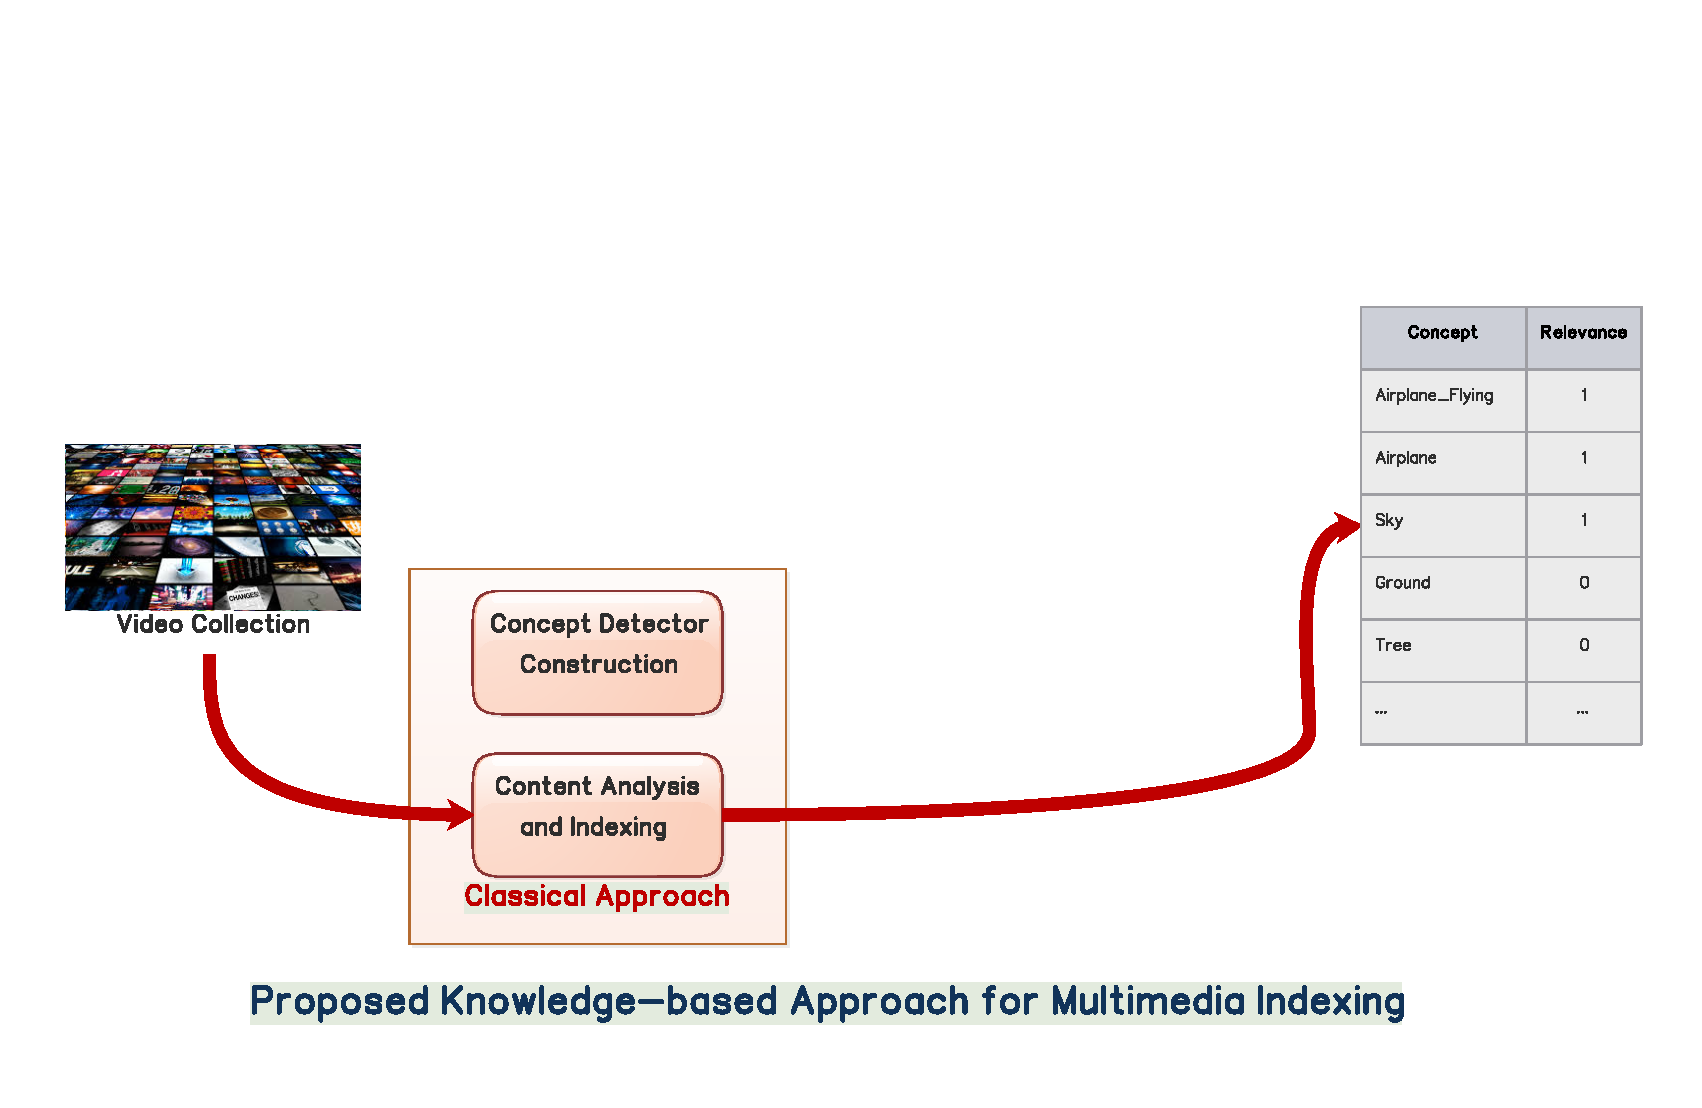
\includegraphics[scale=0.35]{graphics/contribution/contrib_overview_1} \end{center}}
	\only<2>{ \begin{center}\hspace*{-1cm} 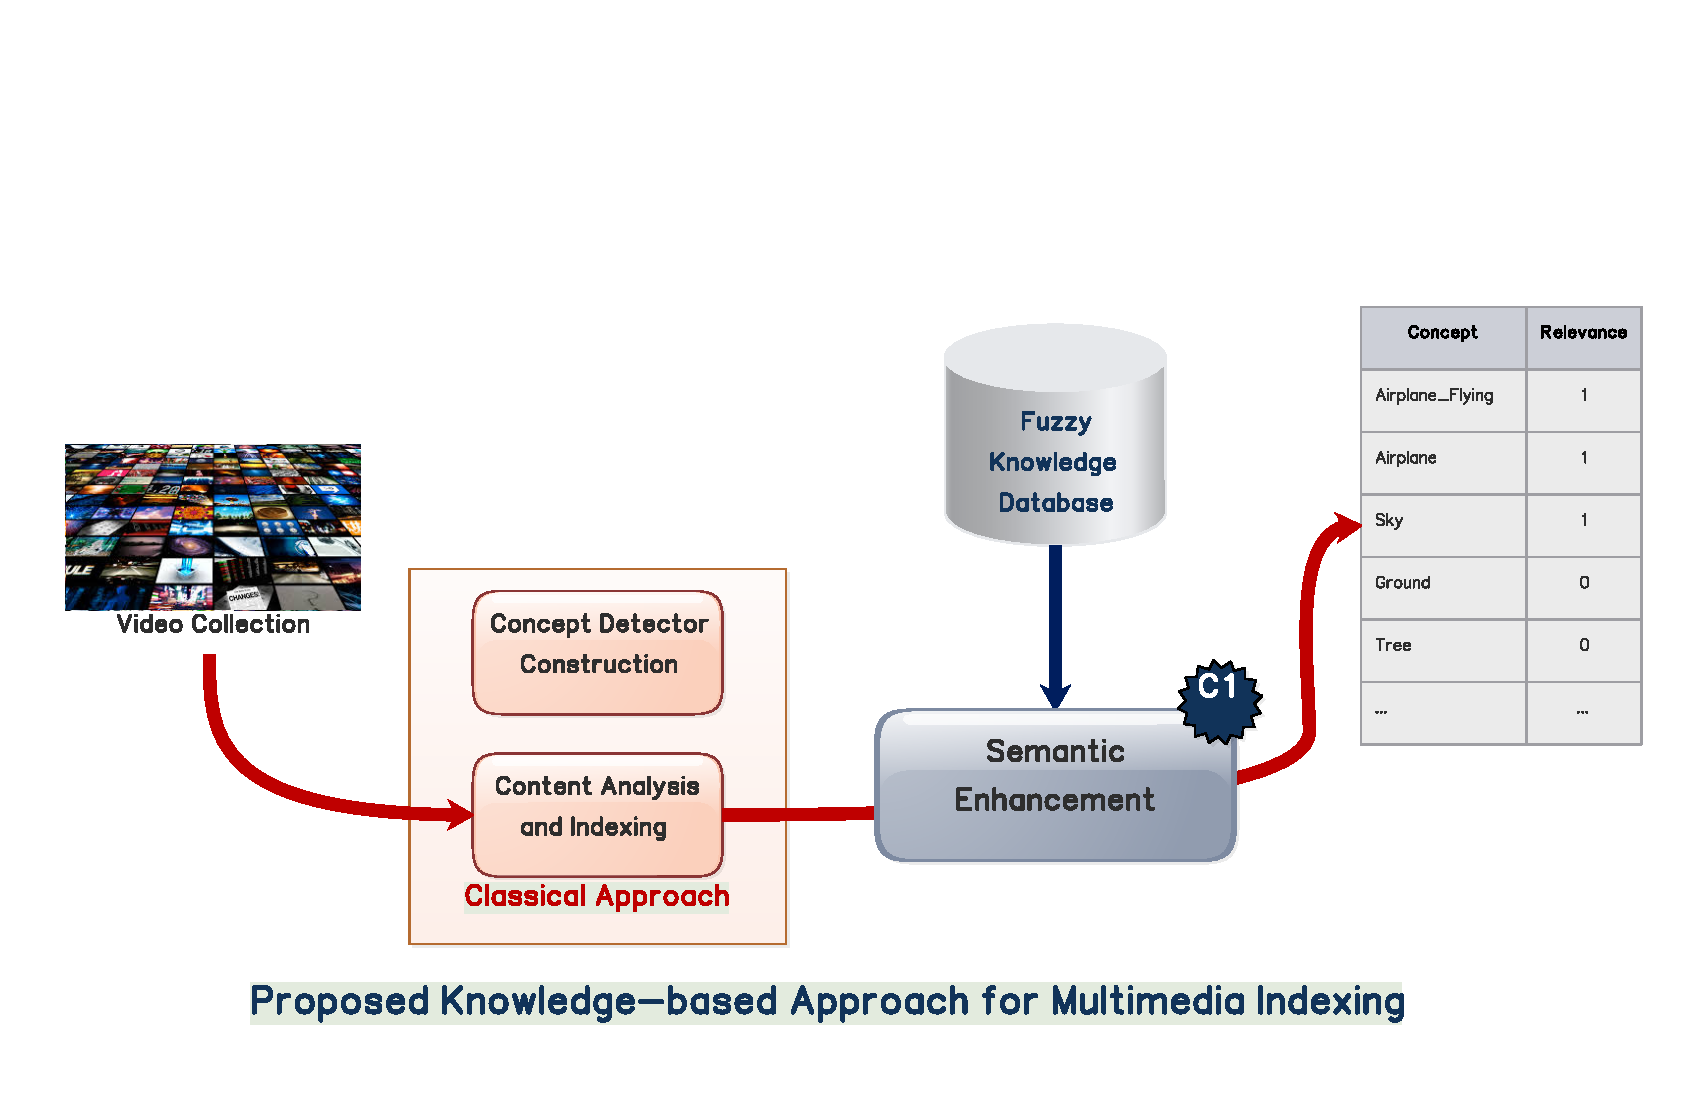
\includegraphics[scale=0.35]{graphics/contribution/contrib_overview_2} \end{center}}
	\only<3>{ \begin{center}\hspace*{-1cm} 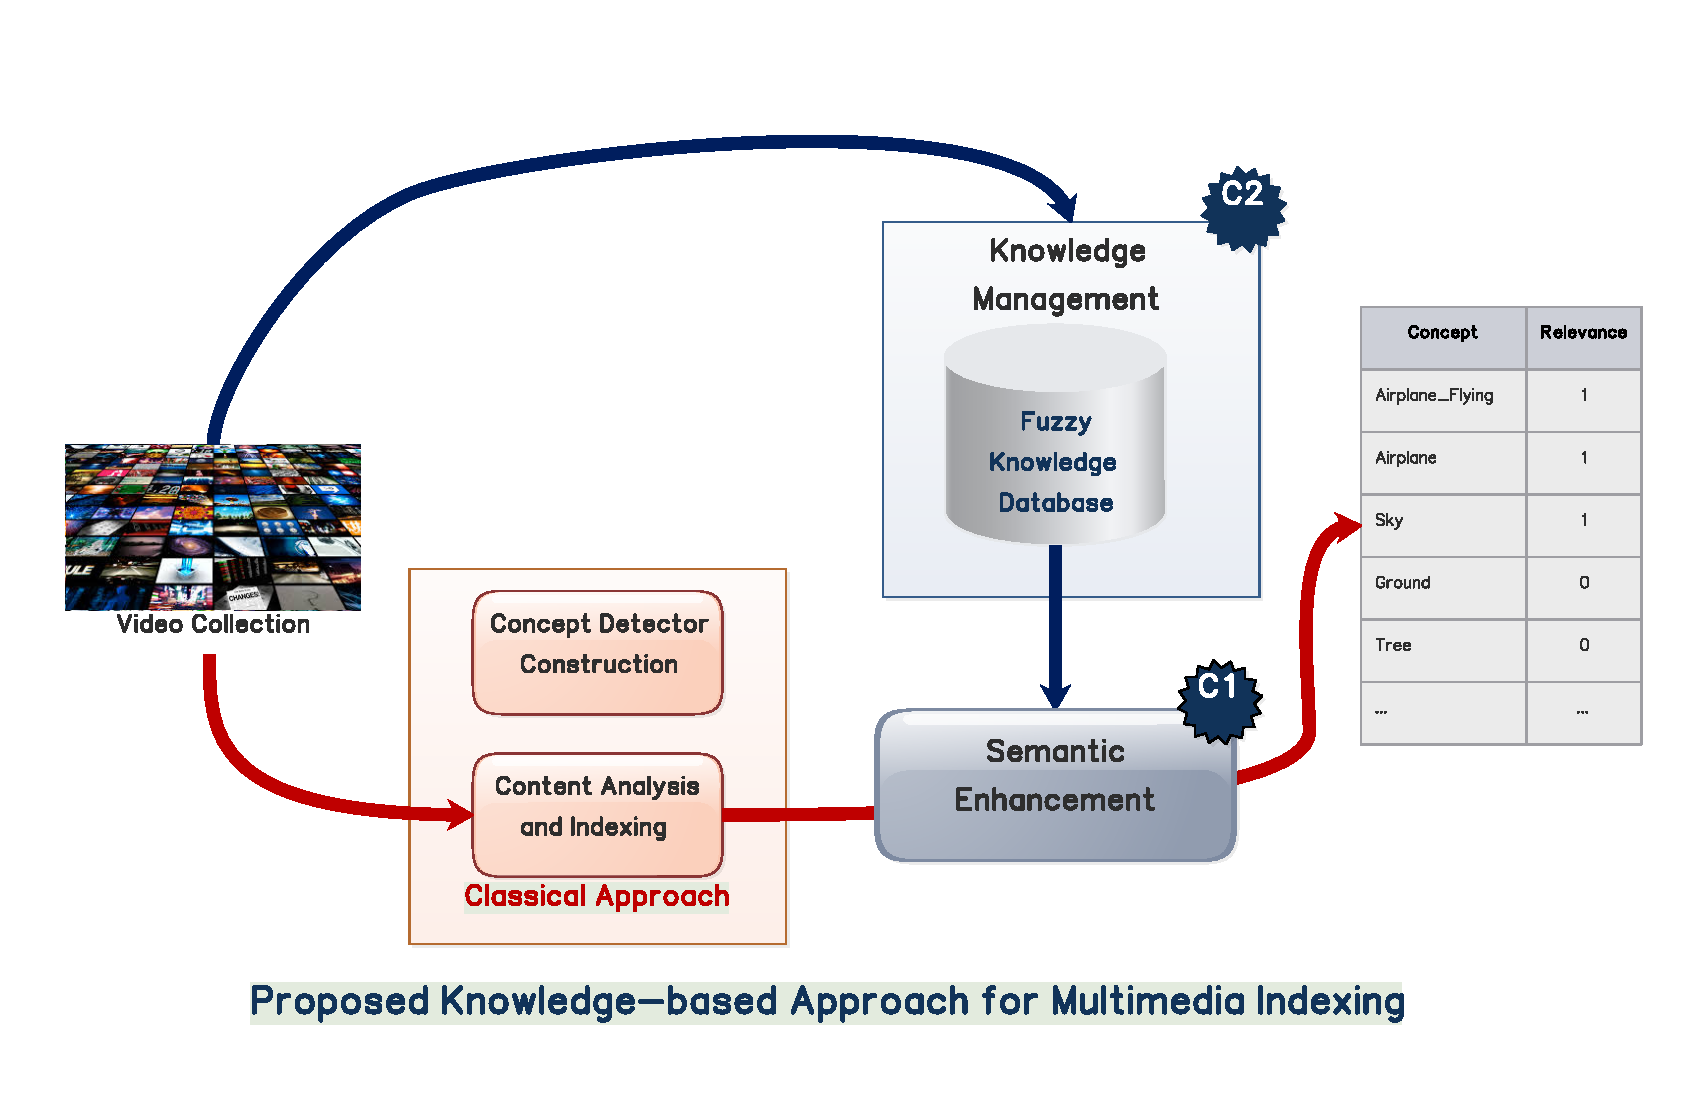
\includegraphics[scale=0.35]{graphics/contribution/contrib_overview_3} \end{center}}
	\only<4>{ \begin{center}\hspace*{-1cm} 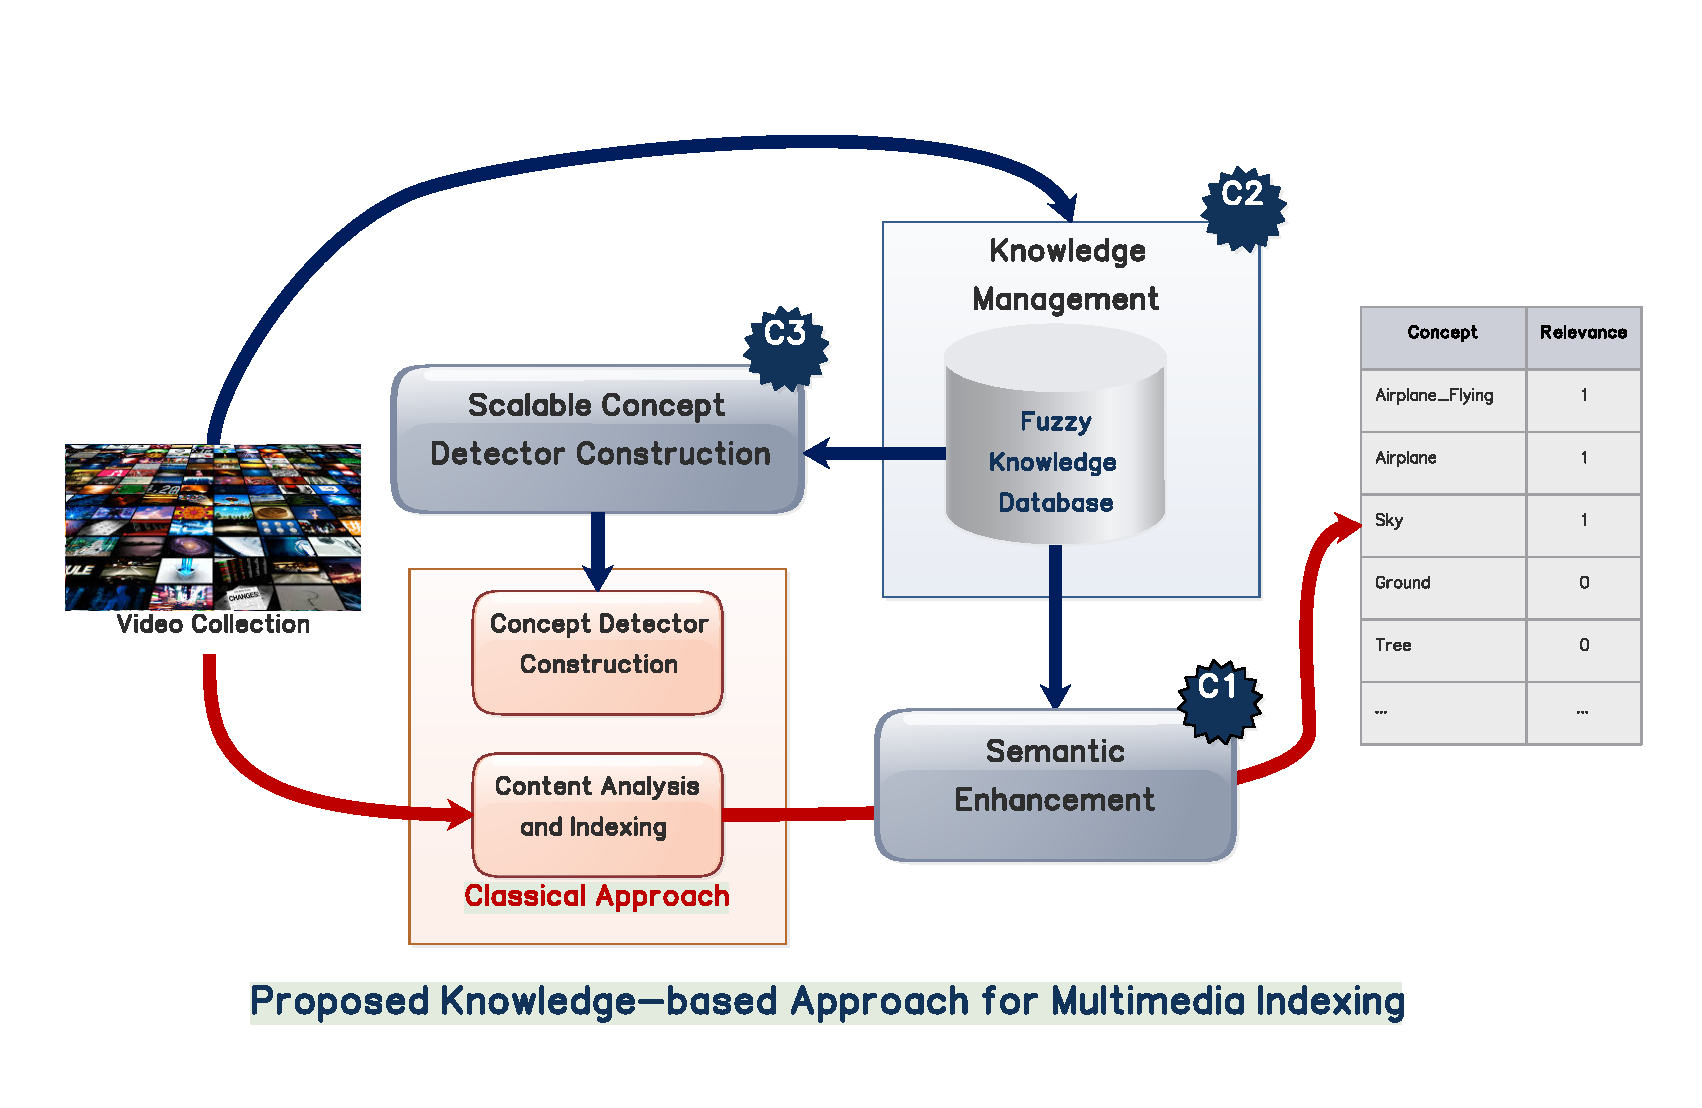
\includegraphics[scale=0.35]{graphics/contribution/contrib_overview_4} \end{center}}

% 	\only<1>{ \begin{center}\hspace*{-1cm} 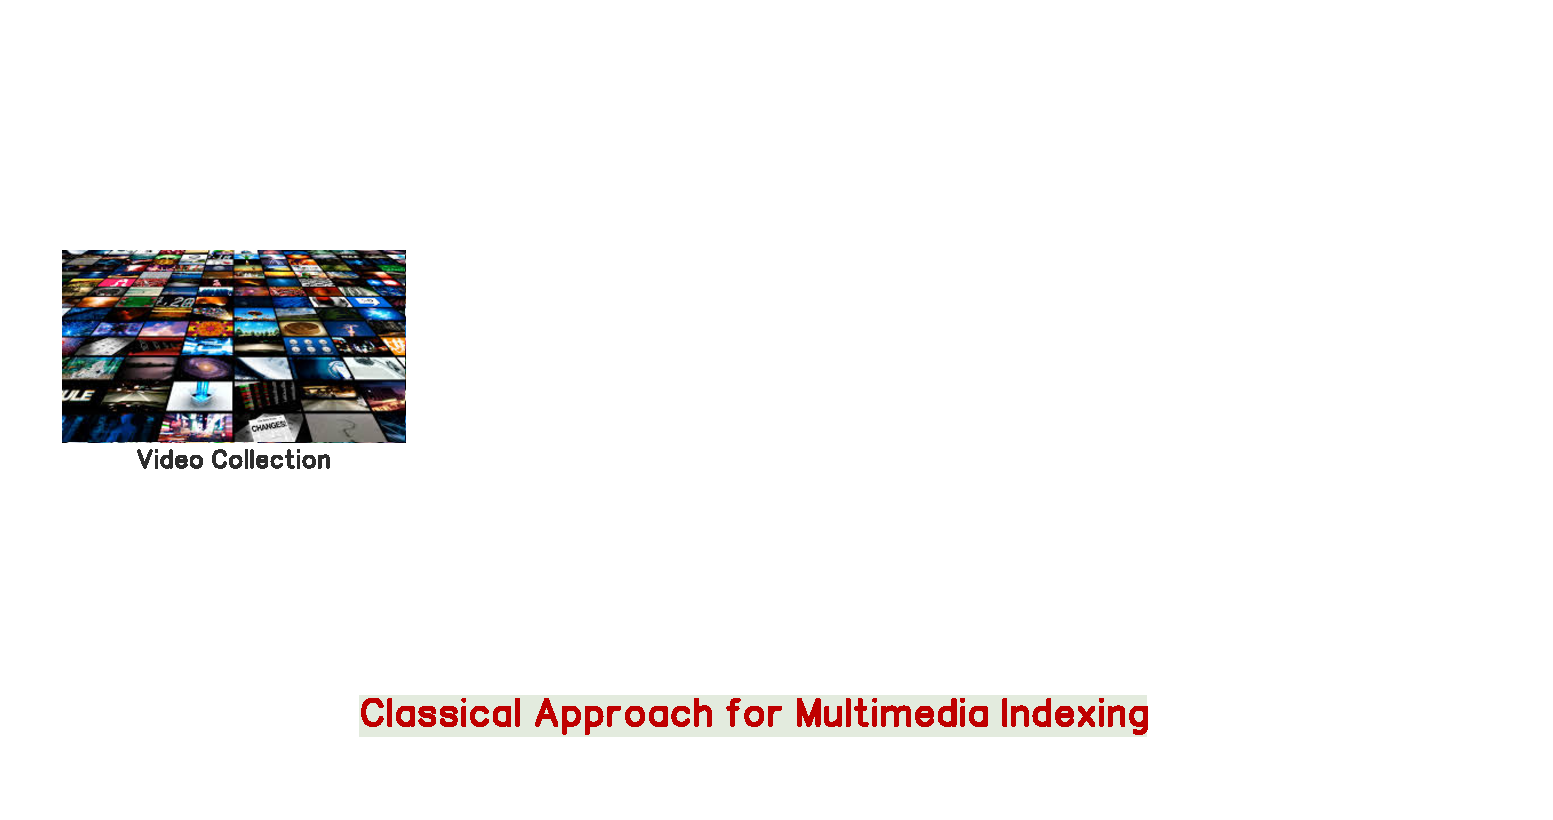
\includegraphics[scale=0.43]{graphics/contribution/contribution_1_1} \end{center}}
% 	\only<2>{ \begin{center}\hspace*{-1cm} 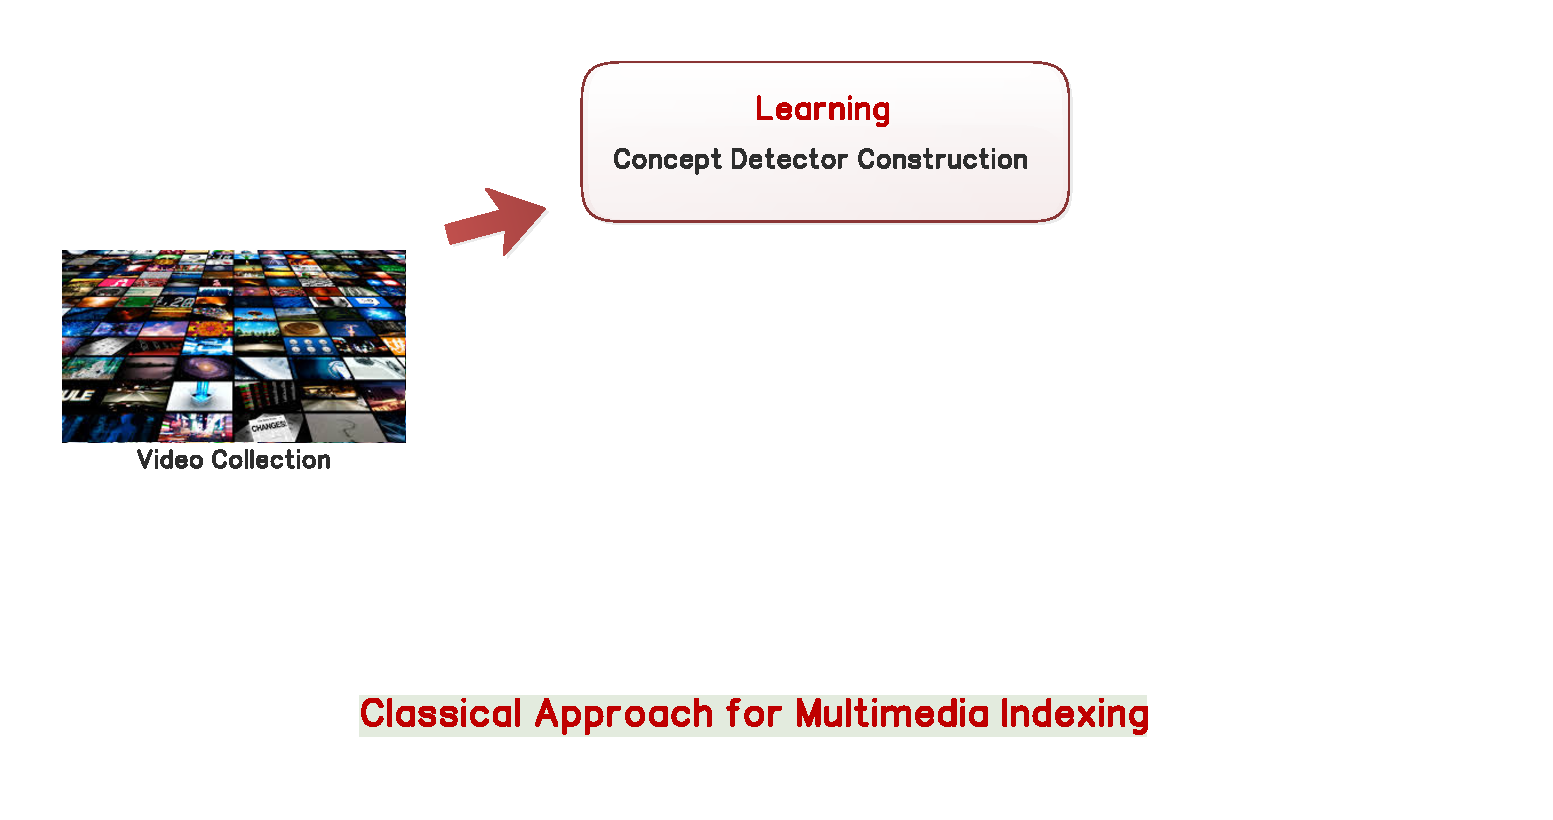
\includegraphics[scale=0.43]{graphics/contribution/contribution_1_2} \end{center}}
% 	\only<3>{ \begin{center}\hspace*{-1cm} 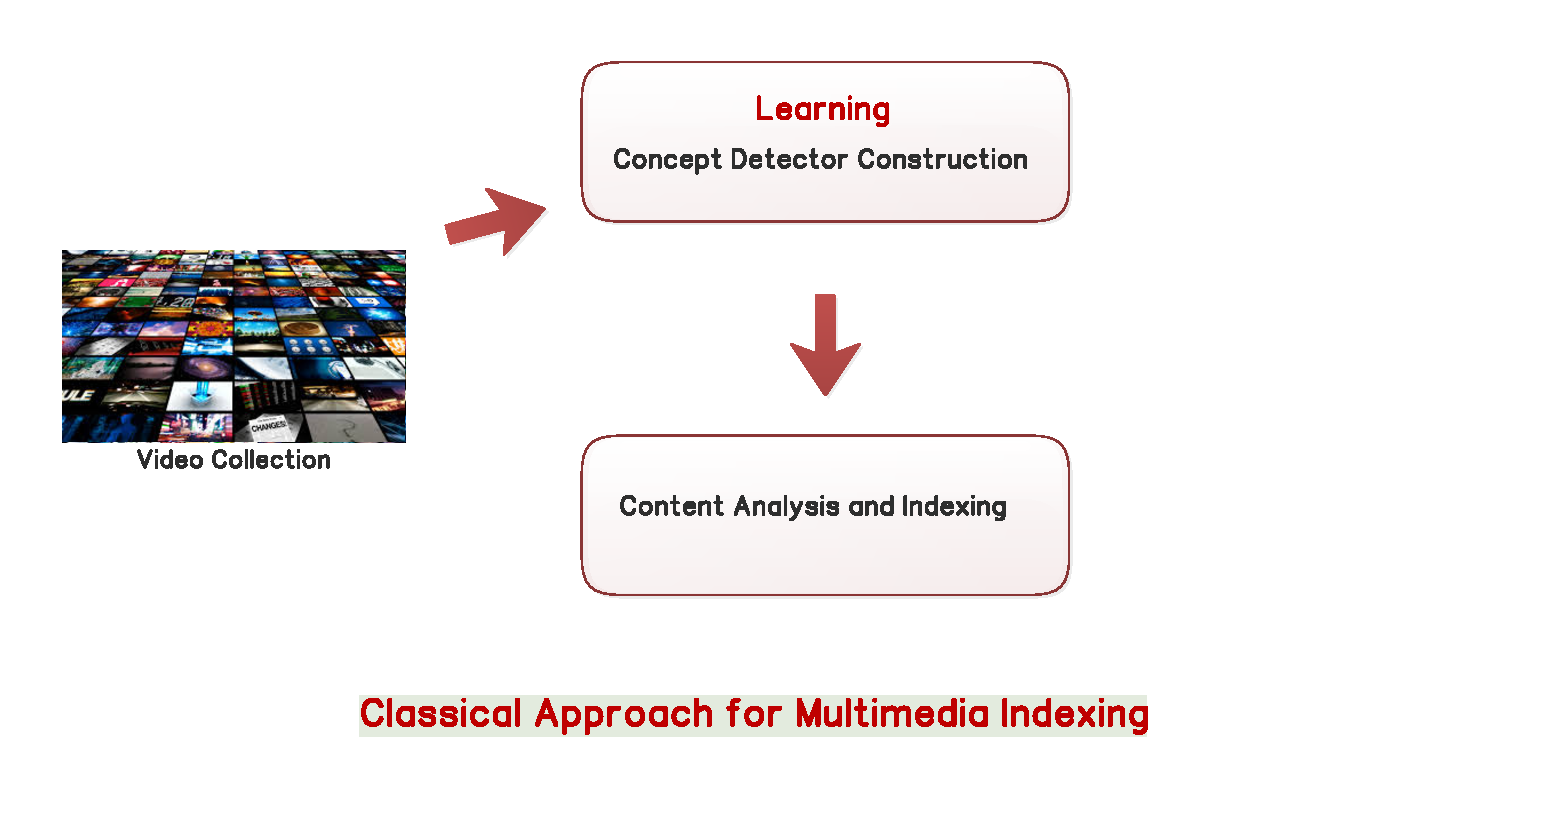
\includegraphics[scale=0.43]{graphics/contribution/contribution_1_3} \end{center}}
% 	\only<4>{ \begin{center}\hspace*{-1cm} 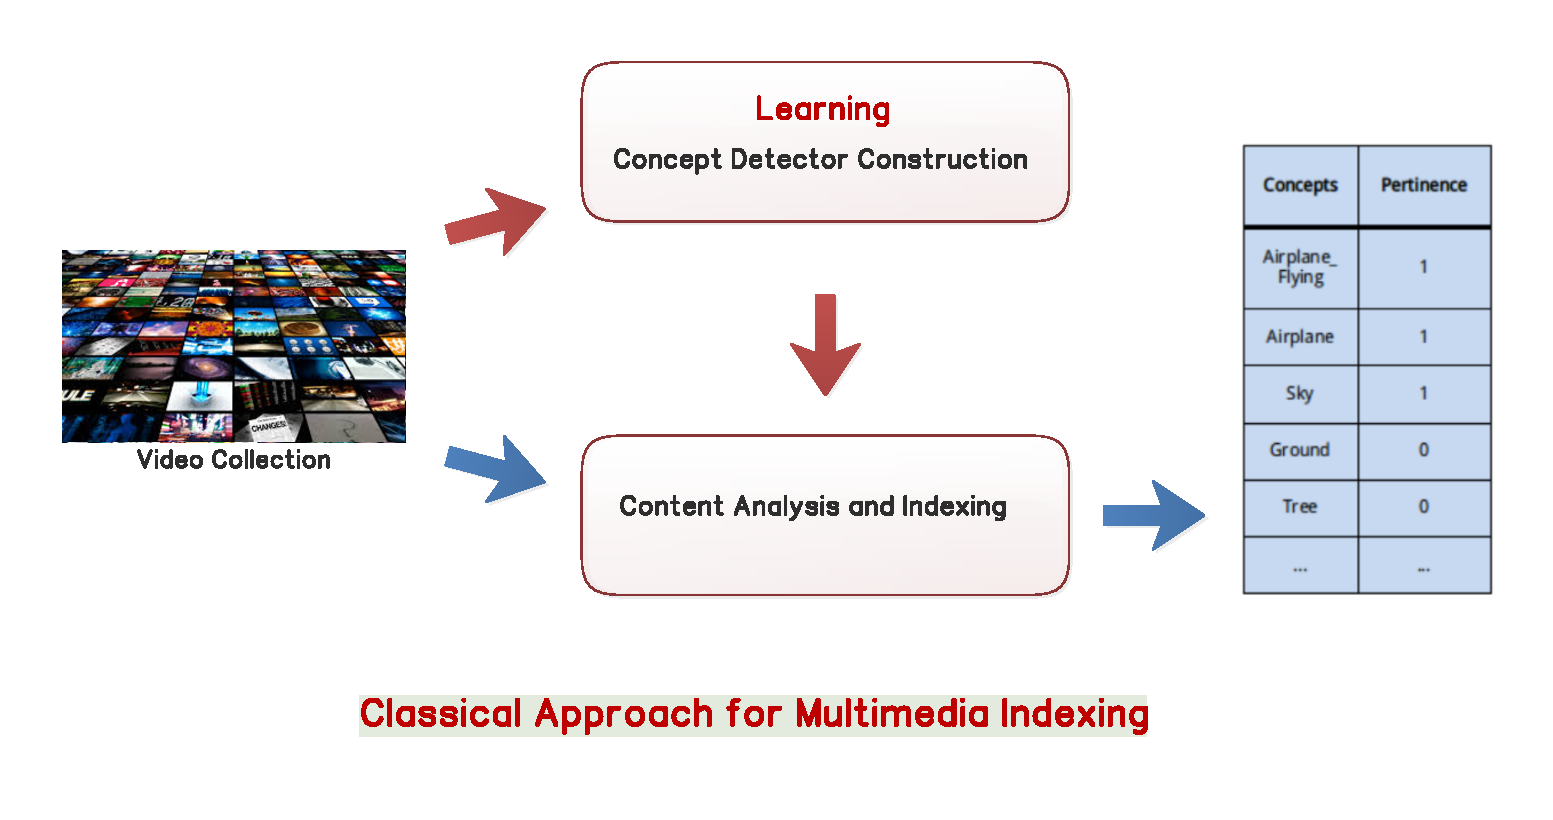
\includegraphics[scale=0.43]{graphics/contribution/contribution_1_4} \end{center}}

% 	\only<5>{ \begin{center}\hspace*{-1cm} 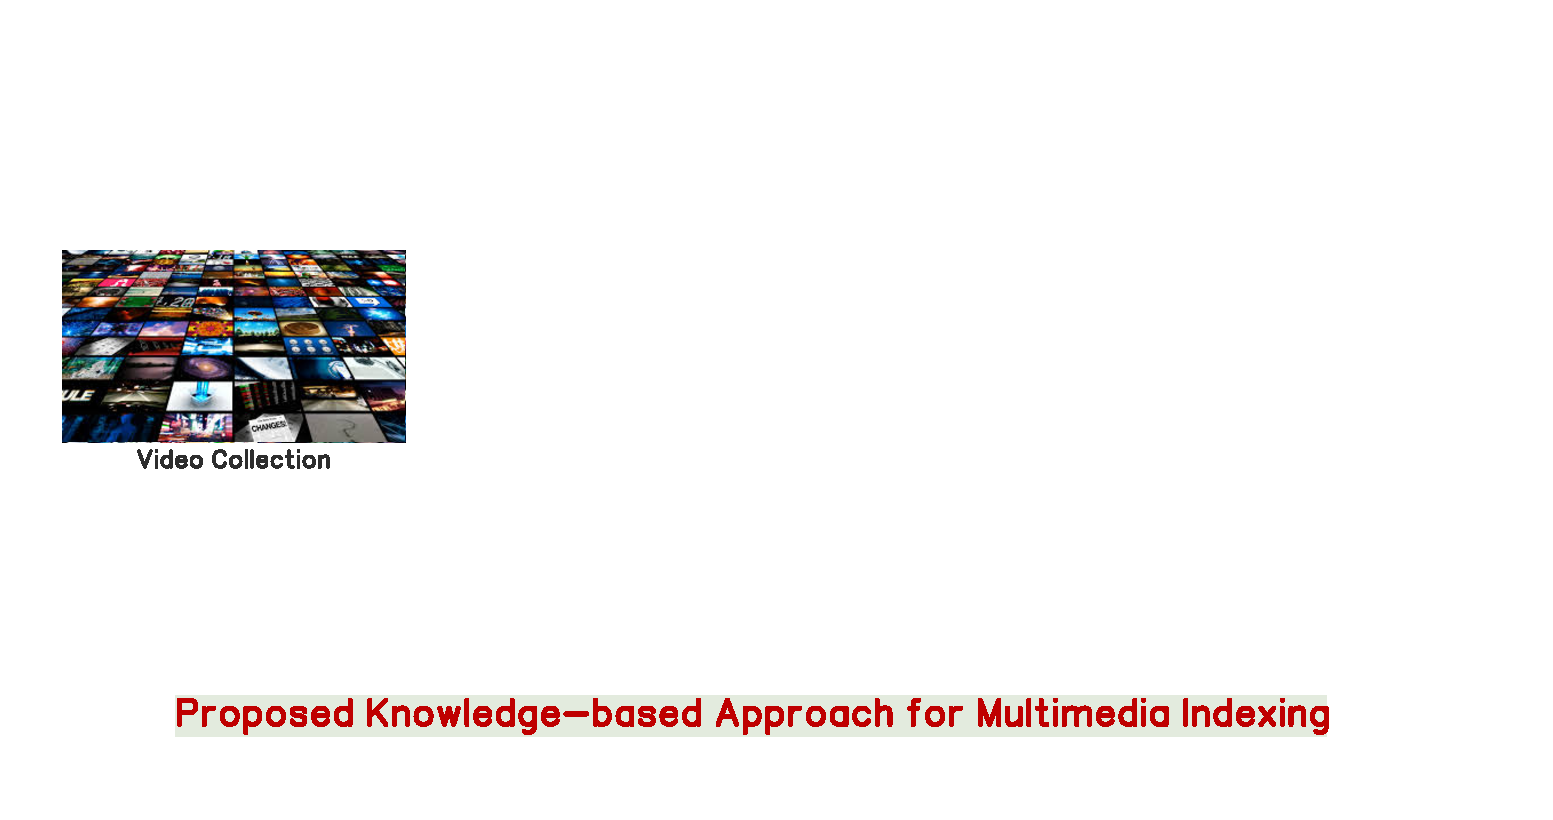
\includegraphics[scale=0.43]{graphics/contribution/contribution_2_0} \end{center}}
% 	\only<6>{ \begin{center}\hspace*{-1cm} 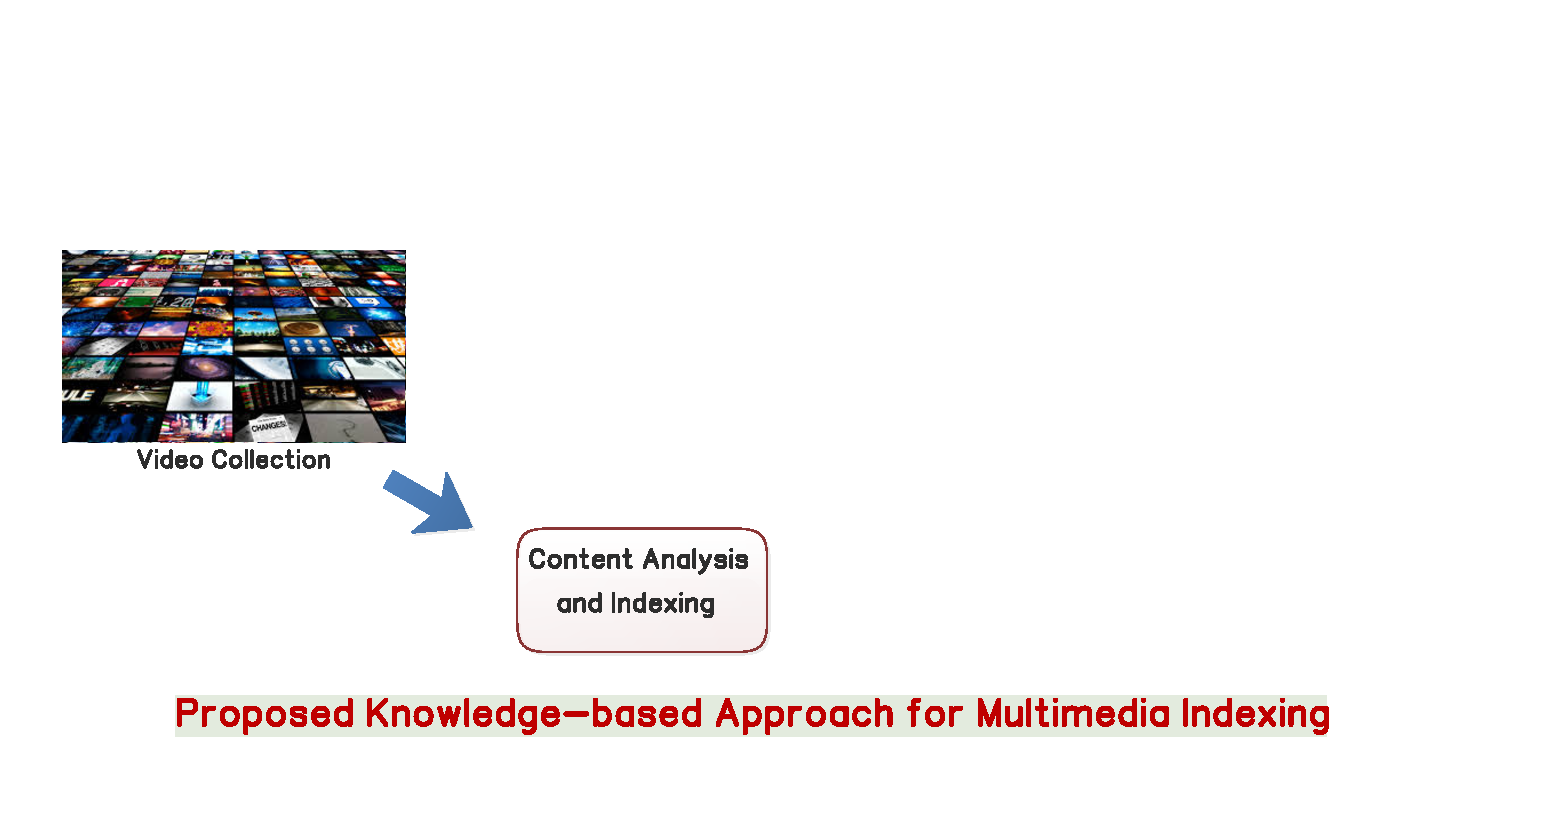
\includegraphics[scale=0.43]{graphics/contribution/contribution_2_1} \end{center}}
% 	\only<7>{ \begin{center}\hspace*{-1cm} 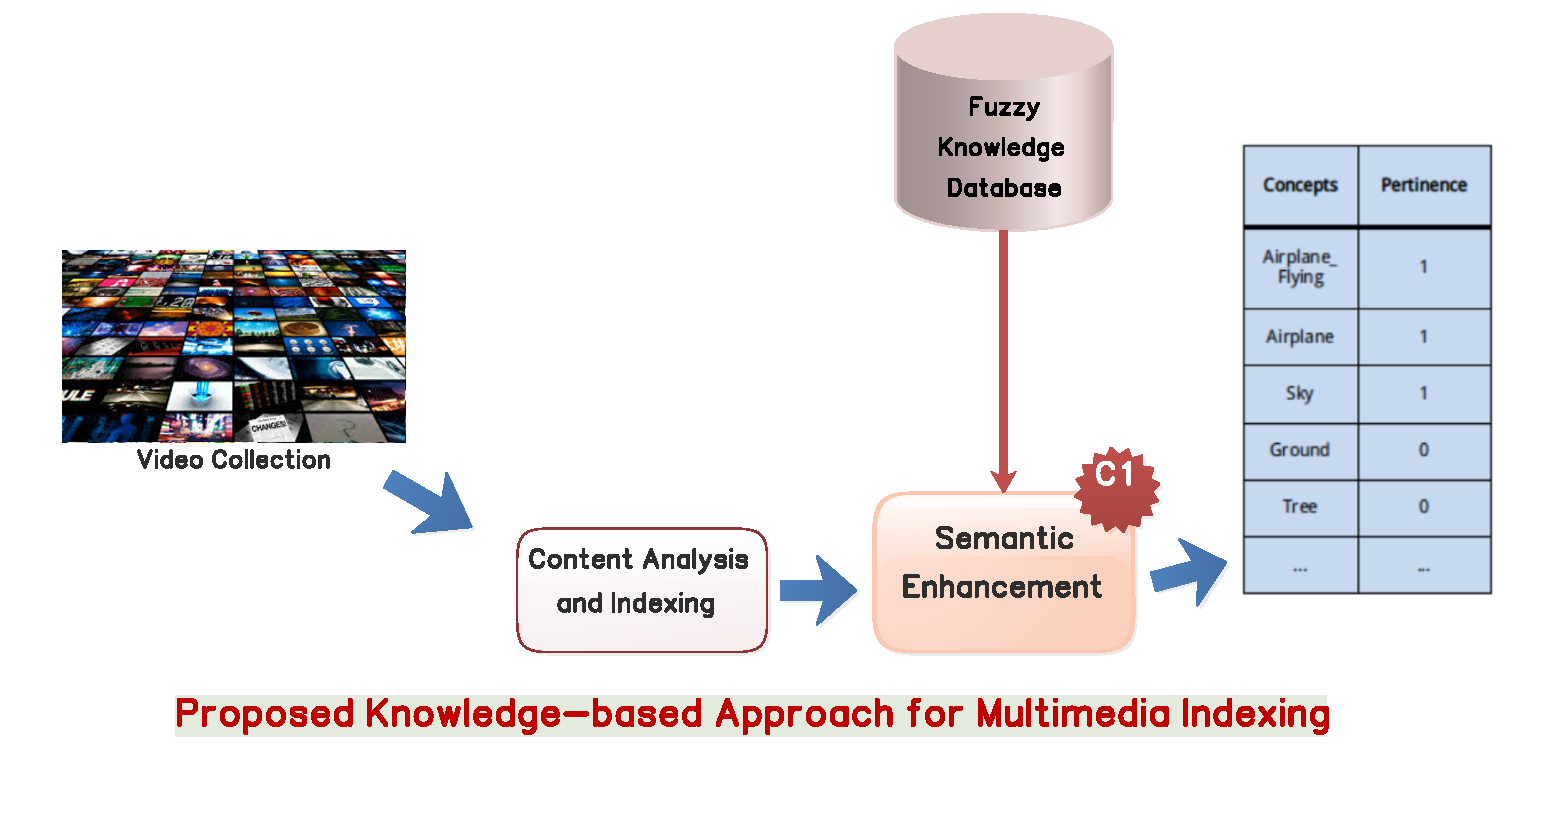
\includegraphics[scale=0.43]{graphics/contribution/contribution_2_2} \end{center}}
% 	\only<8>{ \begin{center}\hspace*{-1cm} 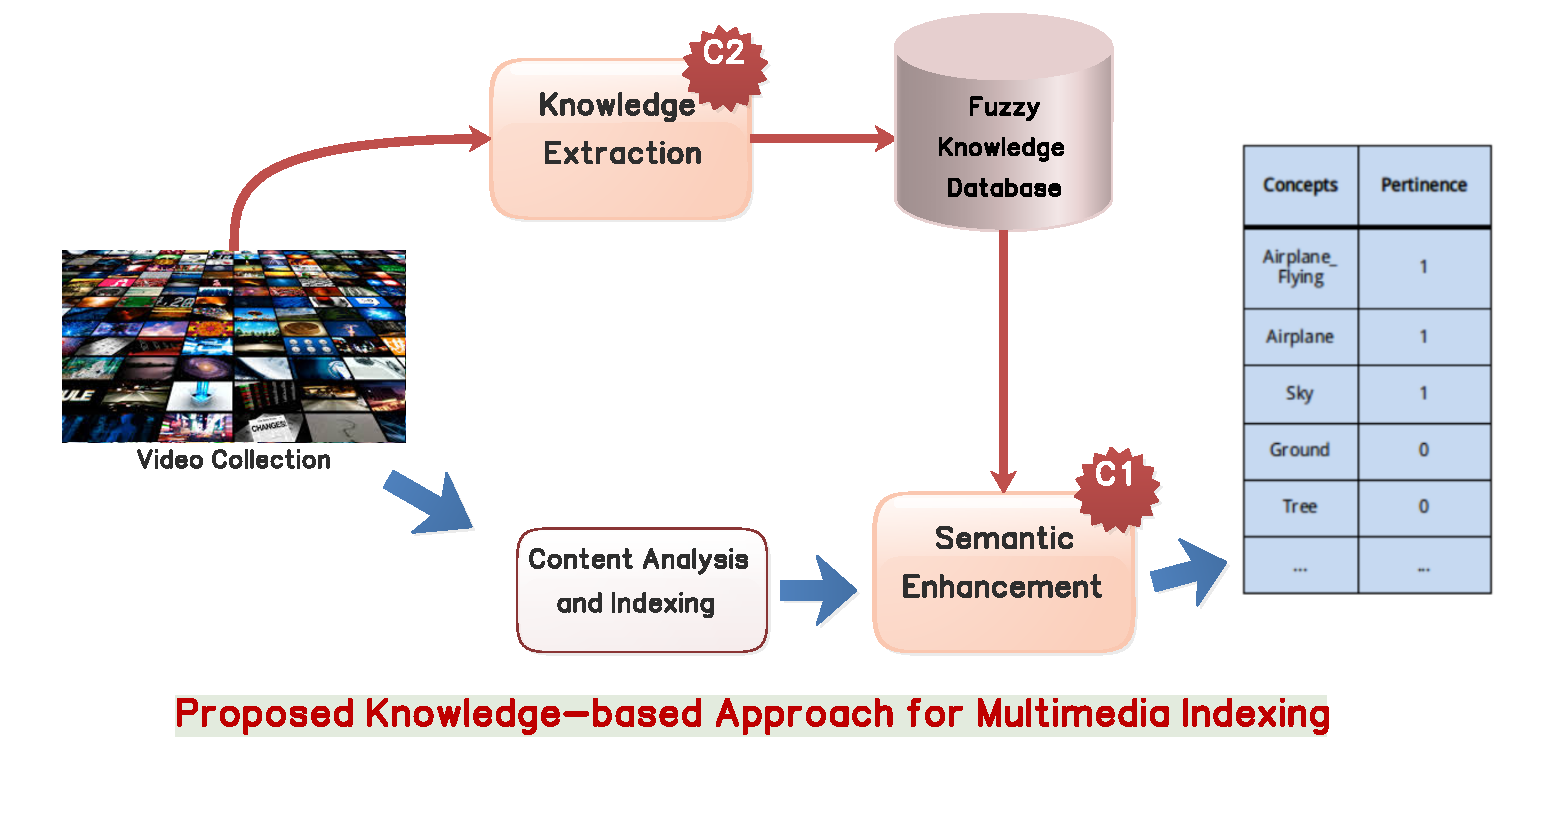
\includegraphics[scale=0.43]{graphics/contribution/contribution_2_3} \end{center}}
% 	\only<9>{ \begin{center}\hspace*{-1cm} 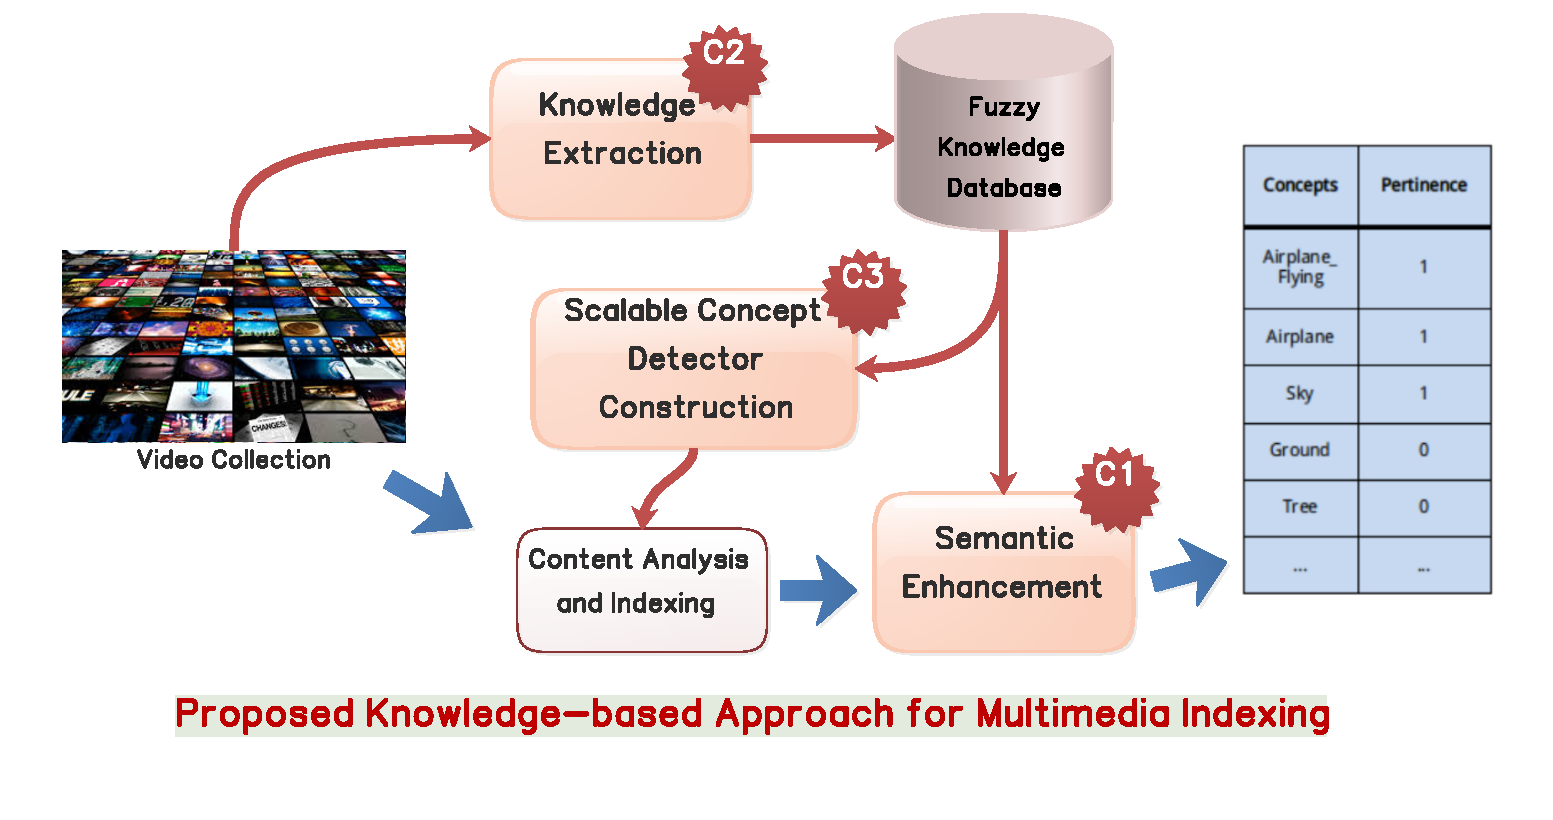
\includegraphics[scale=0.43]{graphics/contribution/contribution_2_4} \end{center}}
\end{frame}

		\subsection[$C_{1}$ Fuzzy knowledge-based Framework for Video Indexing]
				{$C_{1}$ Fuzzy knowledge-based framework for multimedia indexing}
			\begin{frame}
	\frametitle{$C_{1}$: Knowledge-based Approach for Video Indexing}
	\begin{itemize}
	  \small
	  \item $C_{1}$ : A \alert{Knowledge-Based} Framework for video Indexing,
	  \item Capitalize on Semantic \alert{Concepts/Contexts relationships}.
	\end{itemize}
	\begin{center}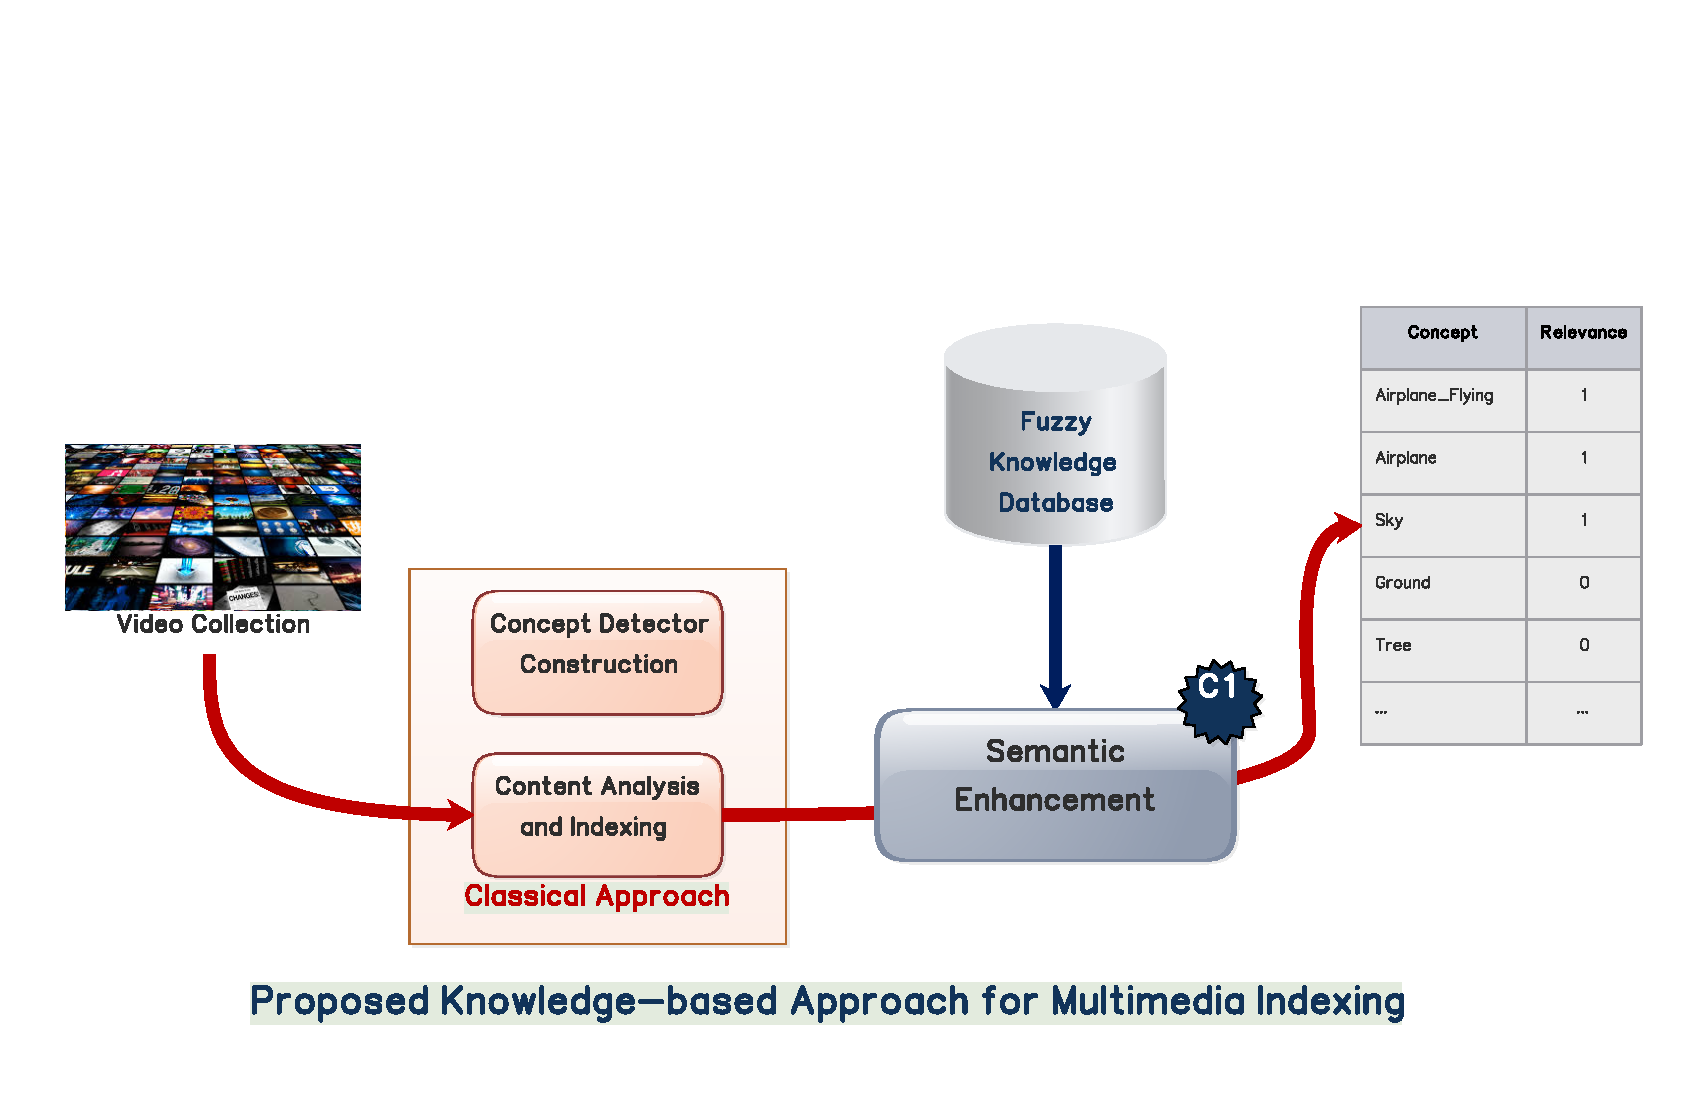
\includegraphics[scale=0.30]{graphics/contribution/contrib_overview_2} \end{center}

\end{frame}

\begin{frame}
	\frametitle{The JDL/Dfs data fusion model \citep{Waltz1990}}
	\only<1>{\hspace*{-1cm}\centering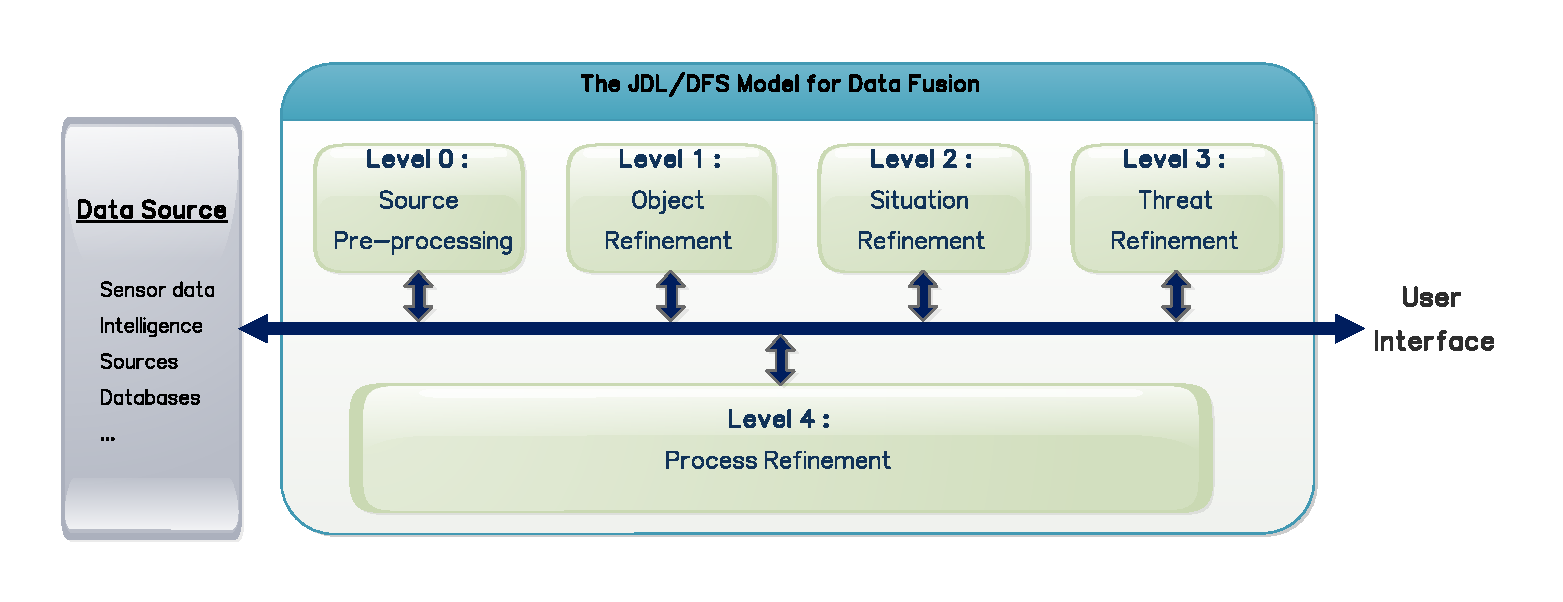
\includegraphics[scale=0.47]{graphics/c1/JDL}}
	\only<2>{\hspace*{-1cm}\centering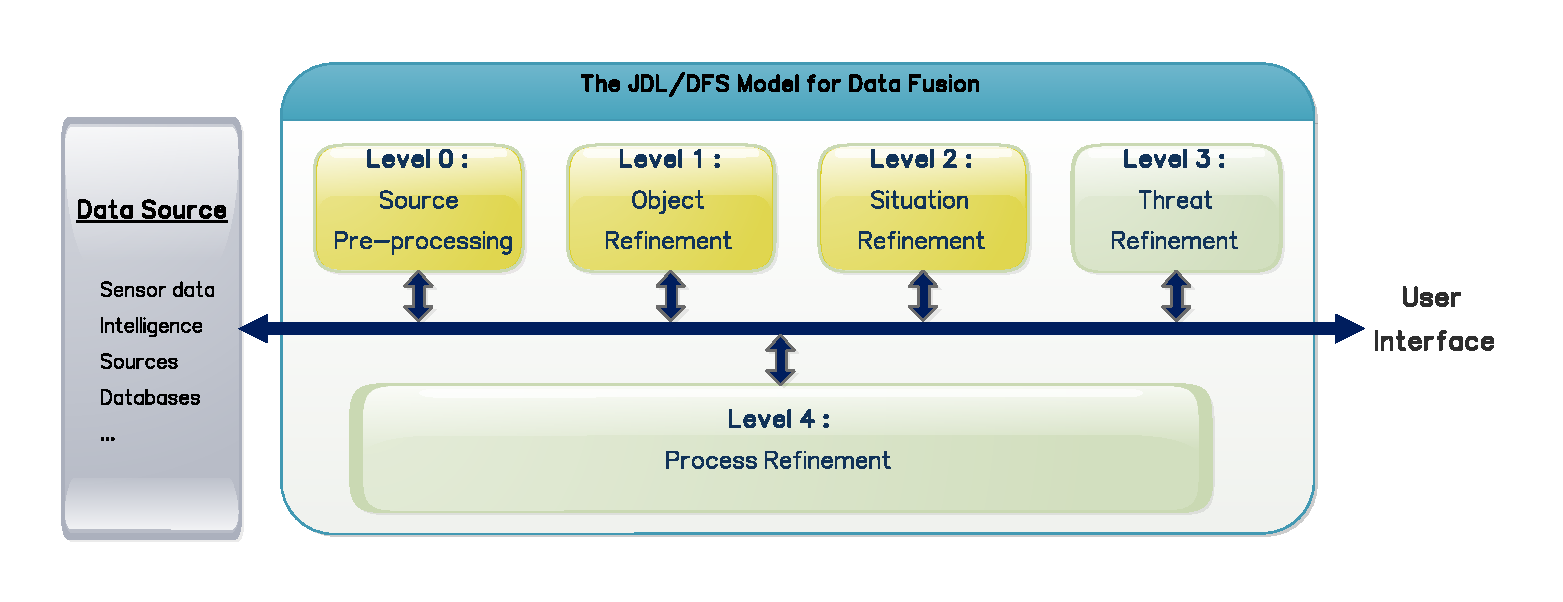
\includegraphics[scale=0.47]{graphics/c1/JDL2}}
\end{frame}
% \begin{frame}
% 	\frametitle{$C_{1}$: Proposed Approach}
	%\only<1>{\hspace*{-1cm}\centering
\includegraphics[scale=0.42]{graphics/c1/JDL_regimvid_1}}
	%\only<2>{\hspace*{-1cm}\centering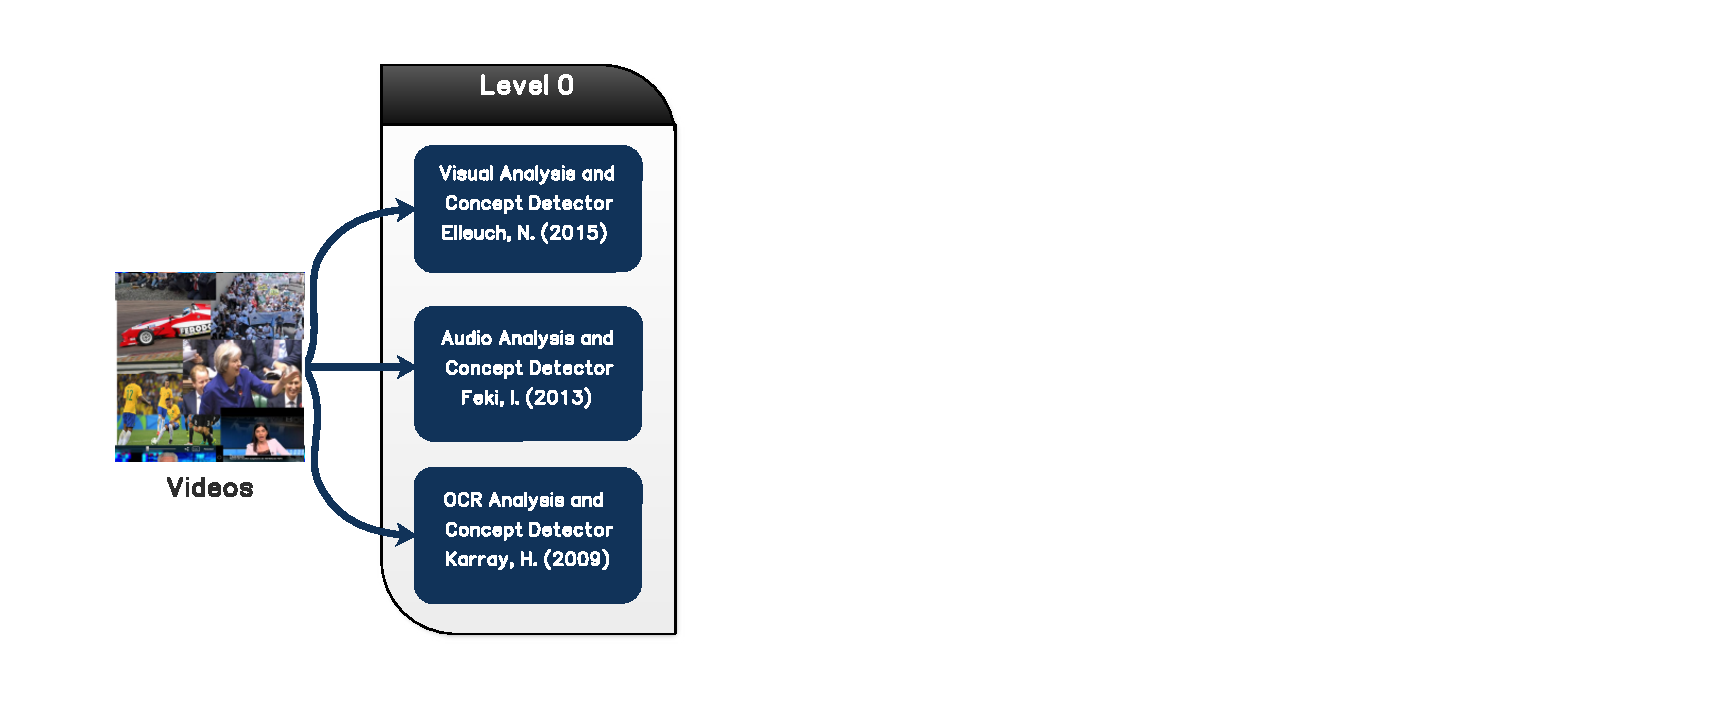
\includegraphics[scale=0.42]{graphics/c1/JDL_regimvid_2}}
	%\only<3>{\hspace*{-1cm}\centering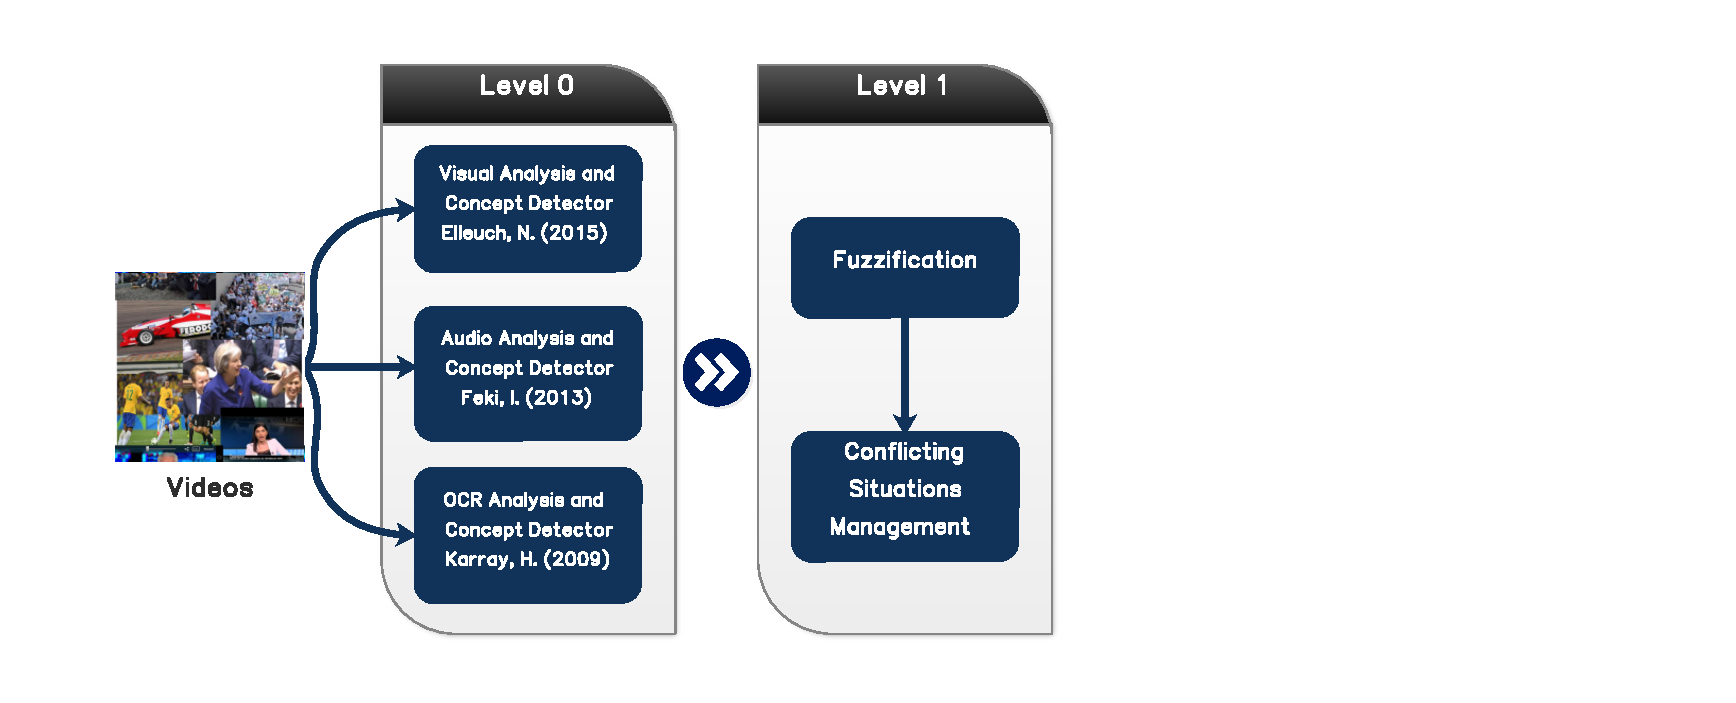
\includegraphics[scale=0.42]{graphics/c1/JDL_regimvid_3}}
% 	\only<4>{\hspace*{-1cm}\centering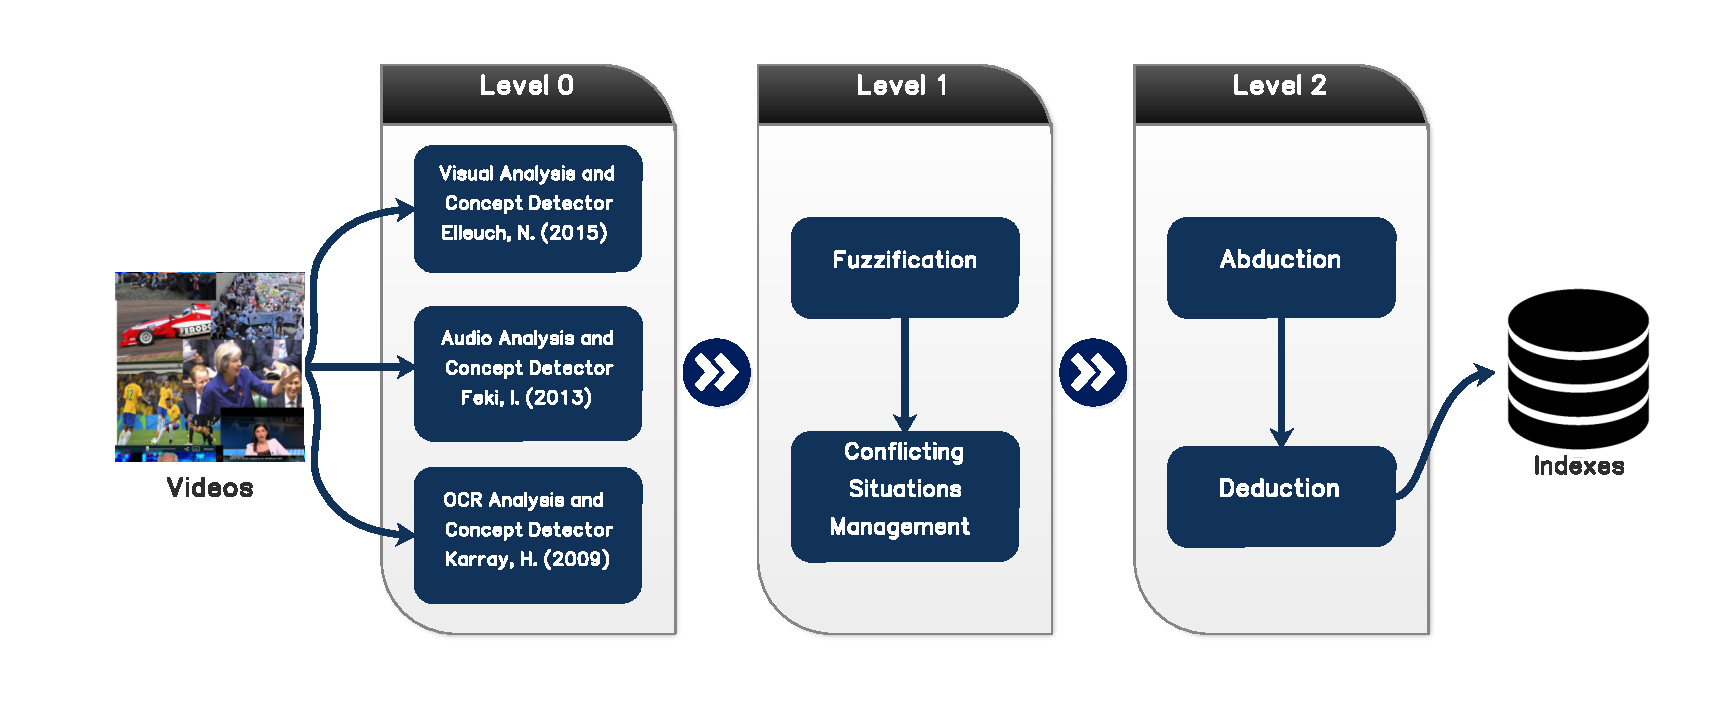
\includegraphics[scale=0.42]{graphics/c1/JDL_regimvid_4}}
%  	{\hspace*{-1cm}\centering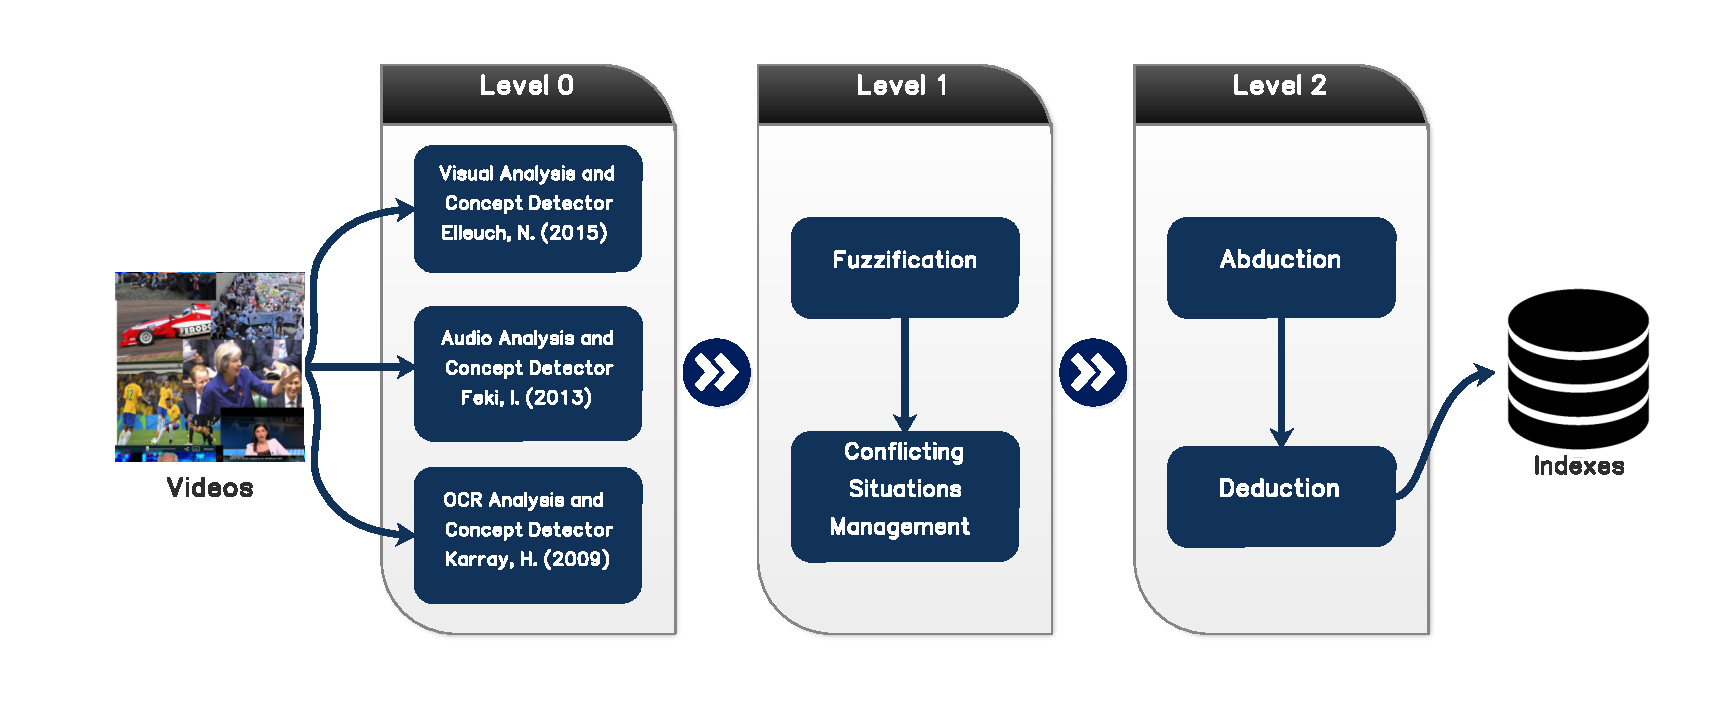
\includegraphics[scale=0.42]{graphics/c1/JDL_regimvid_4}}

% \end{frame}

\begin{frame}
	\frametitle{$C_{1}$: Proposed Approach - Level 0 (Pre-Processing)}
	\small
	\begin{block}{}
		\begin{itemize}
% 			\item Analyze the video content in order to identify semantic concepts
% 			\item The analyzed video is segmented into shots
% 			\item Each shot is labeled by a set of semantic concepts
			\item Level done within these thesis works:
				\begin{description}
					\item[Visual:] Elleuch, N. (2015)
					\item[Audio:] Feki, I. (2013)
					\item[Text/OCR:] Karray, H. (2009)
				\end{description}
		\end{itemize}
	\end{block}
	{\centering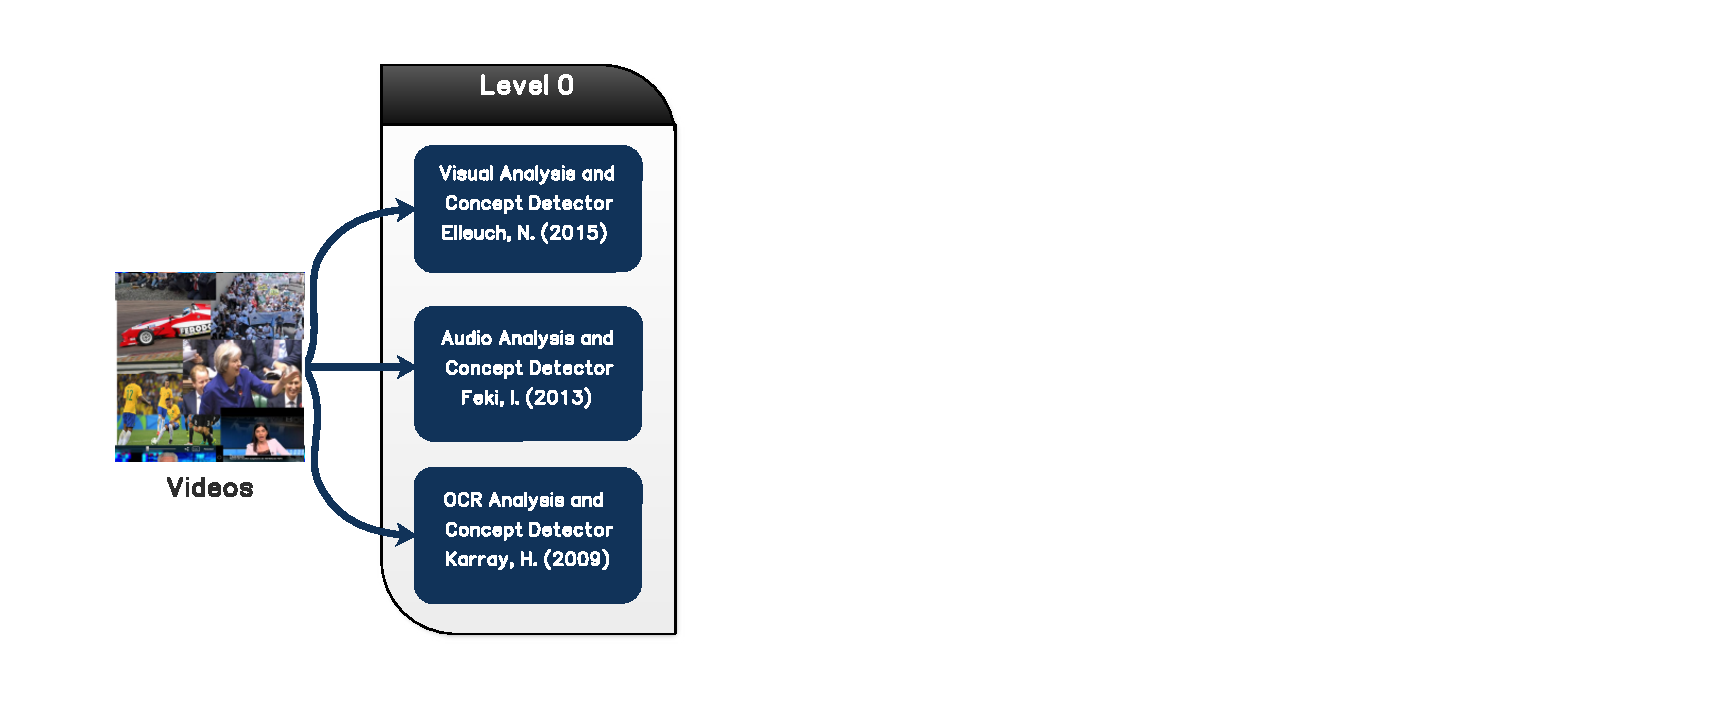
\includegraphics[scale=0.36]{graphics/c1/JDL_regimvid_2}}
\end{frame}

\begin{frame}
	\frametitle{$C_{1}$: Proposed Approach - Level 1 (Object Refinement)}
	\small
	\begin{block}{}
		\begin{description}
			\item[Step 1-Fuzzification:] Rank based fuzzification,
			\item[Step 2-Conflicting Situations Management:]
			       A confidence degree for each modality:
			       $\mu(c) = \alpha \mu_{1}(c) +  \beta \mu_{2}(c) +  \gamma \mu_{3}(c)$ \\where $\alpha + \beta + \gamma= 1$
		\end{description}
	\end{block}
	{\centering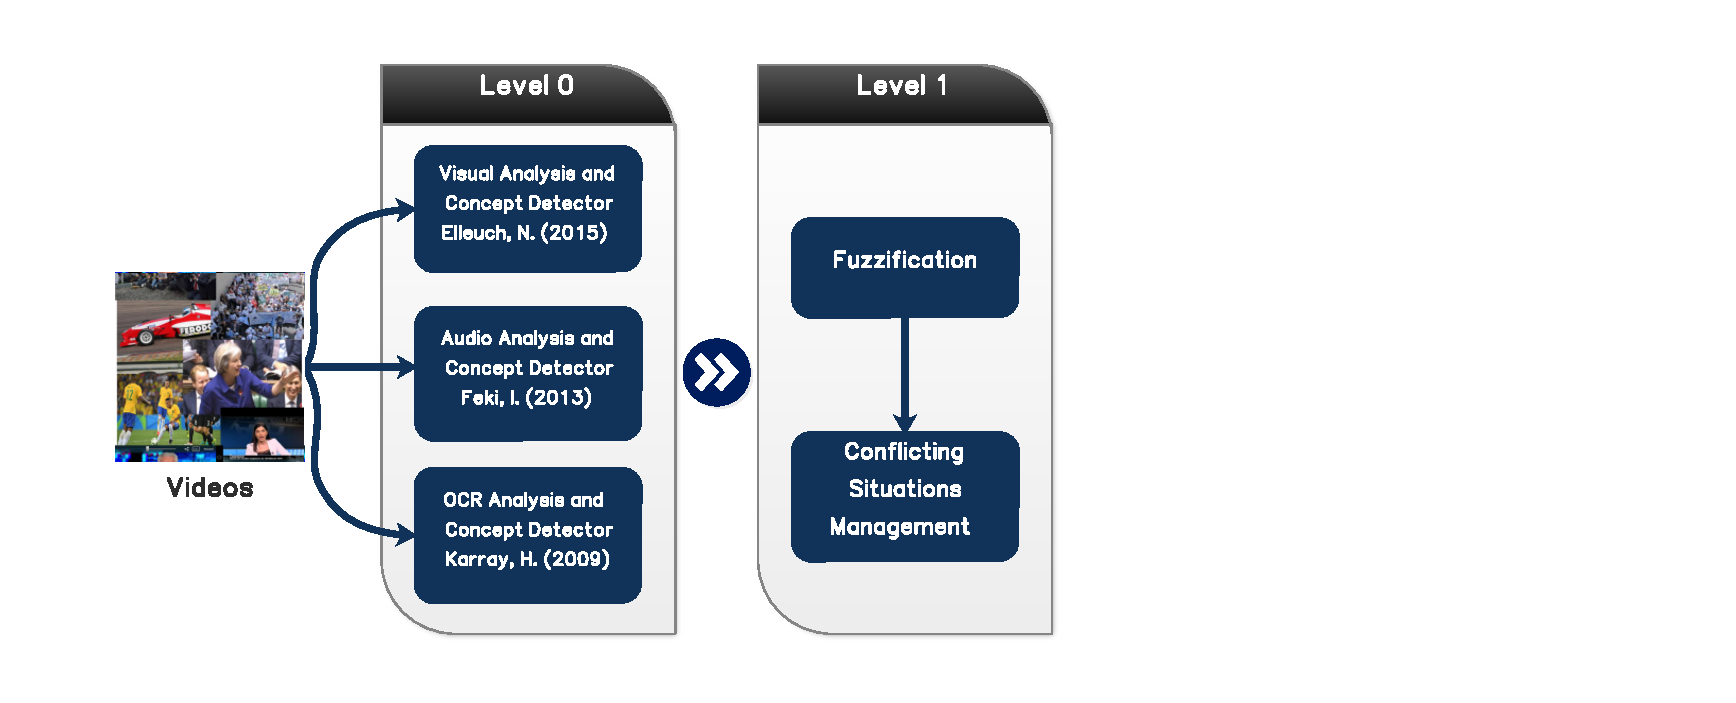
\includegraphics[scale=0.36]{graphics/c1/JDL_regimvid_3}}
\end{frame}

\begin{frame}
	\frametitle{$C_{1}$: Proposed Approach - Level 2 (Situation Refinement)}
	\small
	\begin{block}{}
		Avail of the knowledge dataset capabilities:
		\begin{description}
			\item[Abduction:] Looks for new valuable Knowledge,
			\item[Deduction:] Looks for implicit concepts by analyzing detected explicit ones.
		\end{description}
	\end{block}
	\only<1>{{\centering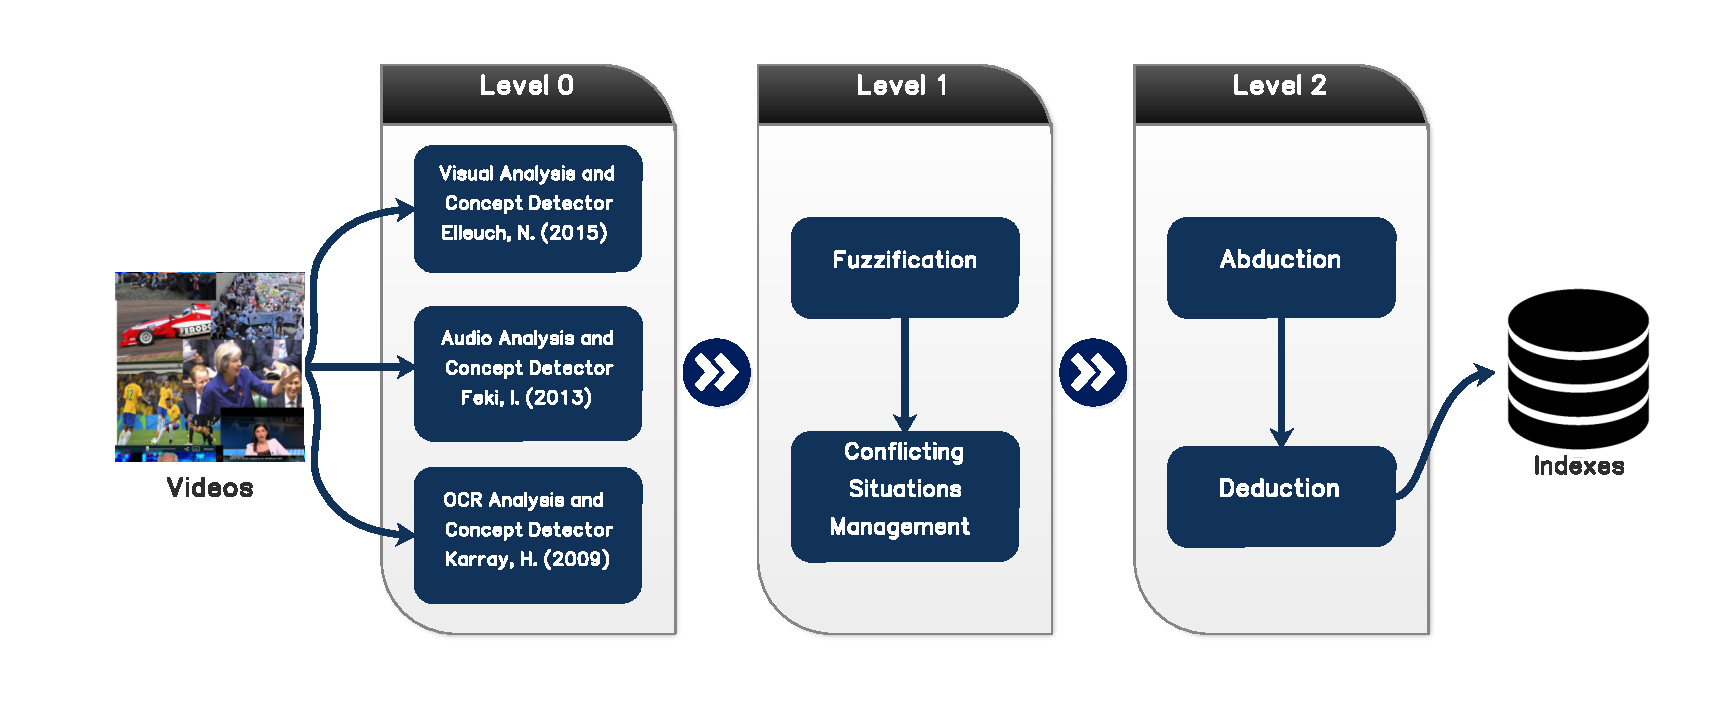
\includegraphics[scale=0.36]{graphics/c1/JDL_regimvid_4}}}
	\only<2>{\begin{columns}
  		\begin{column}{0.49\textwidth}
       		%\begin{block}{Deduction Engine}
			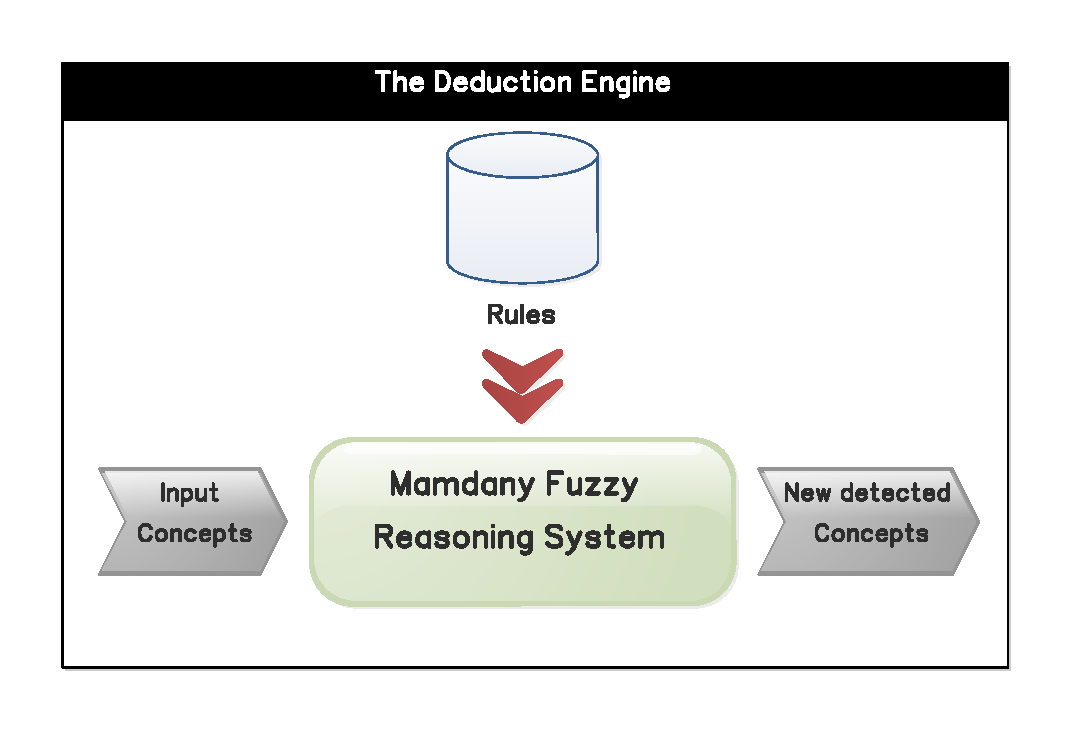
\includegraphics[scale=0.33]{graphics/c1/deduction}
		%\end{block}
    		\end{column}
    		\begin{column}{0.49\textwidth}
       		%\begin{block}{Abduction Engine}
			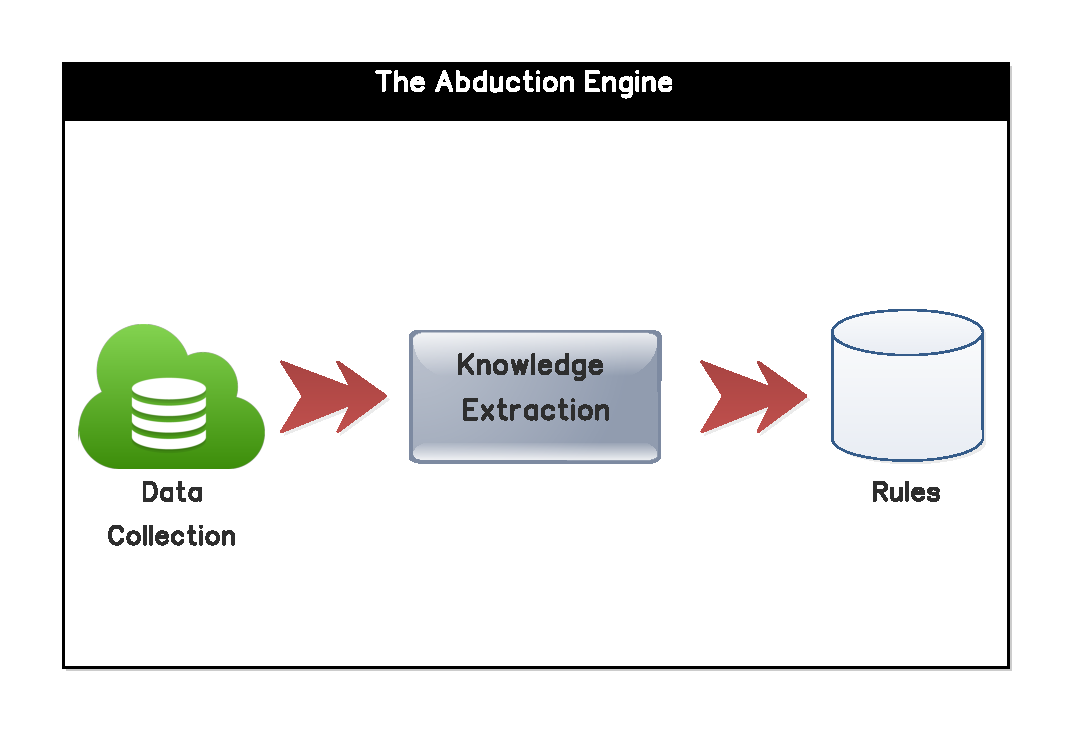
\includegraphics[scale=0.33]{graphics/c1/abduction}
		%\end{block}
    		\end{column}
	\end{columns}
	}
\end{frame}


\begin{frame}
	\frametitle{$C_{1}$: Preliminary Experiment I}
	\small
	\begin{exampleblock}{Experimentation Setup}
		\begin{itemize}
			\item \textsc{TrecVid 2010}: $200h$ of video development set and $200h$ of video test set
			\item 130 semantic concepts
		  \end{itemize}
	\end{exampleblock}

	\begin{exampleblock}{Baseline}
		\begin{itemize}
			\item We look to evaluate the semantic enhancement  of a non knowledge-based approach 
			\alert{\citep{Elleuch2010}}
			\item \alert{Visual} semantic indexing
			\item We used the \alert{\textsc{LsCom}} Ontology for the rules
		 \end{itemize}
	\end{exampleblock}
\end{frame}
\begin{frame}
	\frametitle{$C_{1}$: Preliminary Experiment II}
	\small
	{\only<1>{
	\begin{exampleblock}{Accuracy Evaluation}
		\centering
%			\includegraphics[scale=0.6]{graphics/c1_result1}
		\centering
		\tiny
		\begin{tabular}{|l||ccc|ccc|}\hline
				\multirow{1}{*}{\textit{\textbf{Semantic Concepts}}} & 	
				\multicolumn{3}{c}{\textbf{Baseline [Elleuch, N. (2015)]}} & 
				\multicolumn{3}{c|}{\textbf{\alert{Knowledge based}}}\\ 

				& infAP & P & R & infAP & P & R \\
				\hline
				\hline
	
				Outdoor	&	-&	0.52	&	0.59&	-&	\textbf{\alert{0.88}}	& \textbf{\alert{0.77}} \\
				Vegetation& 0.1 & 0.74		& 0.68& 0.1& 0.74 & 0.68  \\
				Landscape& -& 0.6		& 0.79& -& 0.6 & 0.79\\
				Sky& -& 0.66	& 0.9		& -& 0.66& 0.9  \\
				Trees& -& 0.62& 0.72 & - & 0.62 & 0.72\\
				Mountain& -& 0.68 & 0.8 & -  & 0.68 & 0.8  \\
				Ground\_Vehicle& 0.043  & 0.3& 0.66& \textbf{\alert{0.18}} & \textbf{\alert{0.6}} & \textbf{\alert{0.73}}\\
				Road& -& 0.43& 0.6 & -& 0.43& 0.6 \\
				Car  & 0.075 & 0.42 & 0.64& \textbf{\alert{0.17}} & \textbf{\alert{0.58}} & \textbf{\alert{0.73}} \\
				Bus& -& 0.52& 0.73& - & 0.52& 0.73 \\
				Bicycles& 0.142& 0.67& 0.92& \textbf{\alert{0.185}}& \textbf{\alert{0.82}}& \textbf{\alert{0.97}} \\
				Emergency Vehicle& -& 0.9& 0.83& - & 0.9& 0.83\\
				Building& 0.022& 0.18& 0.22& \textbf{\alert{0.1}}& \textbf{\alert{0.5}}& \textbf{\alert{0.43}}  \\
				Truck & -& 0.35& 0.37& -& 0.35& 0.37 \\
				Airplane Flying & 0.102& 0.8 & 0.78& 0.102& 0.8& 0.78                              \\
				Airplane  & -& 0.5& 0.6& -& \textbf{\alert{0.6}}& 0.6  \\
				\hline
		\end{tabular}
	\end{exampleblock}
	\footnotesize
		\begin{block}{}
			Semantic Enhancement of about \alert{$4.8\%$} compared to a classical concept detection [Elleuch, N. (2015)].
		\end{block}
	}}
	{\only<2>{
	\footnotesize
	\begin{exampleblock}{Teams}
		\alert{MediaMill} University of Amsterdam, \alert{PicSoM} University of Helsinki, \alert{Quaero} Europe, 
		\alert{FudaSys} Fuzhou University (China), \alert{Vireo} University of Hong Kong, \alert{IRIM} France, \alert{UC3M} University of Madrid, \dots{}
	\end{exampleblock}
	\begin{exampleblock}{}	
		\centering	
		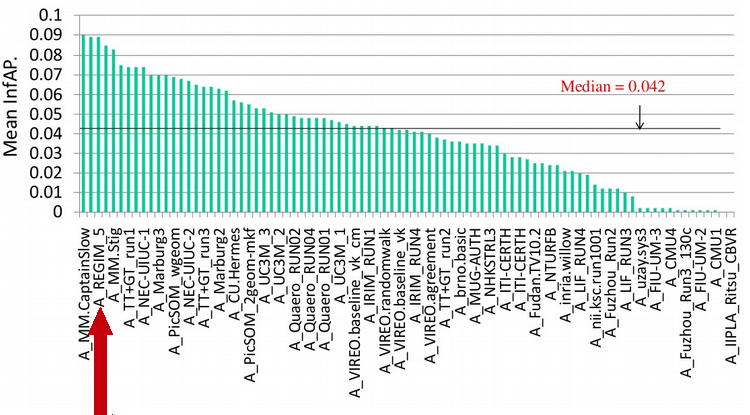
\includegraphics[scale=0.5]{graphics/c1/c1_result2}
	\end{exampleblock}
	}
	}

	
\end{frame}


\begin{frame}
	\frametitle{$C_{1}$: Fuzzy Contextual Ontology}
	\small
	\begin{block}{Motivation}
		\begin{itemize}
			\item Defining an \alert{ontology} more semantically richer than \textsc{LsCom},
			\item Introducing the semantic \alert{context}.
		  \end{itemize}
	\end{block}
	\begin{columns}
  		\begin{column}{0.45\textwidth}
       		\begin{block}{Deduction Engine}
			\begin{itemize}
				\item Defining a \alert{contextual space},
				\item \alert{relationships} between contexts and concepts,
				\item a \alert{deduction} engine is used to enhance a semantic interpretation.
			\end{itemize}
		\end{block}
    		\end{column}
    		\begin{column}{0.55\textwidth}
       		%\begin{block}{Abduction Engine}
			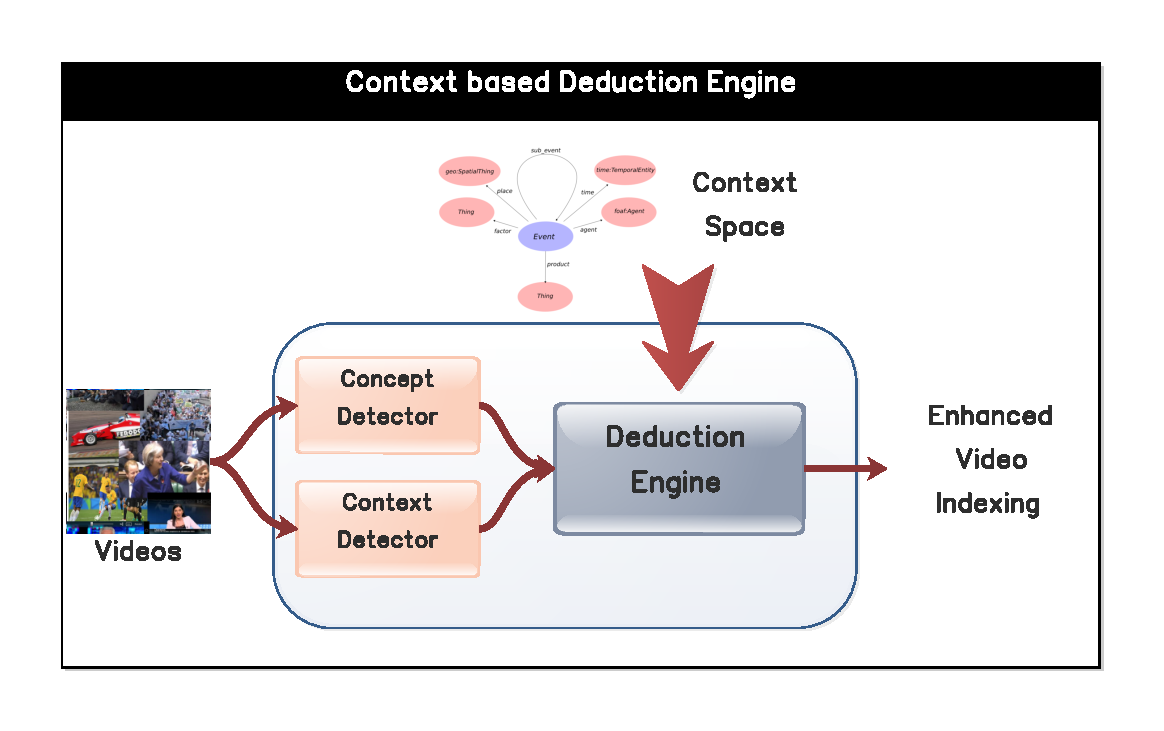
\includegraphics[scale=0.32]{graphics/c1/deduction_contexte}
		%\end{block}
    		\end{column}
	\end{columns}
\end{frame}

\begin{frame}
	\frametitle{$C_{1}$: Fuzzy Contextual Ontology (continued)}
	\footnotesize
	\begin{block}{$O^{f}$: a fuzzy Ontology}
		\begin{itemize}
			\item Let $T$ and $C$ be respectively a set of semantic contexts and concepts.
			\item Let $Q$ be a set of the fuzzy qualifiers: \alert{``weak''} and \alert{``strong''}. 
			\item We define four relationships :
			\begin{center} 
							\begin{tiny} 
							\begin{tabular}{c|c|c|c} 
								\hline\textbf{ \textit{Name}} & \textbf{\textit{Symbol}} & 
								\textbf{\textit{Meaning}} & \textbf{\textit{Type}} \\ 
					
								\hline Generalization & $t_{i}:t_{j} $ & 
								The concept $c_{i}$ is the generalization of the concept $c_{j} $ 
				 				&  $TxT$   \\ 
								
								\hline IsRelatedTo 	& $c_{i} |t{k}\rightarrow c_{j}$ &
								The concept $c_{i}$ is related to the concept $c_{j}$ within $t_{k}$ 
				 				& $CxC$  \\ 
					
								\hline IsPartOf 	& $\{c_{i}\} \in t_{j}	$ & 
								A set of concept $c_{i}$ is a part of the context $t_{j}$ 
								& $CxT$ \\ 
					
								\hline Includes 	& $t_{i} \supset c_{j}$	& 
								The context $t_{i}$ includes the concept $c_{j}$ 
				 				&  $TxC$ \\ 
								\hline 
							\end{tabular} 
							\end{tiny} 
							\end{center} 
		 \end{itemize}
	\end{block}
	%\pause
	\begin{block}{$O^{f}$: deduction engine}
		\begin{itemize}
			\item \alert{Strong Rule}: 
				$\alpha'_{k}(c_{j})=\mu_{k}*(max\{P(V_{S_{k}}|c_{i}),P(V_{S_{i}}|t_{k'})\})*\mu_{Strong}(\alpha_{k})$
			\item \alert{Weak Rule}: 
				$\alpha'_{k}(c_{j})=\mu_{k}*(min\{P(V_{S_{k}}|c_{i}),P(V_{S_{i}}|t_{k'})\})*\mu_{Weak}(\alpha_{k})$
		\end{itemize}
	\end{block}
\end{frame}

\begin{frame}
	\frametitle{$C_{1}$: Second Experimentation}
	\small
	\begin{exampleblock}{Experimentation Setup}
		\begin{itemize}
			\item \textsc{TrecVid 2010} dataset
		  \end{itemize}
	\end{exampleblock}
	\begin{exampleblock}{The $O^{f}$ ontology: Defined by Experts}
		\centering 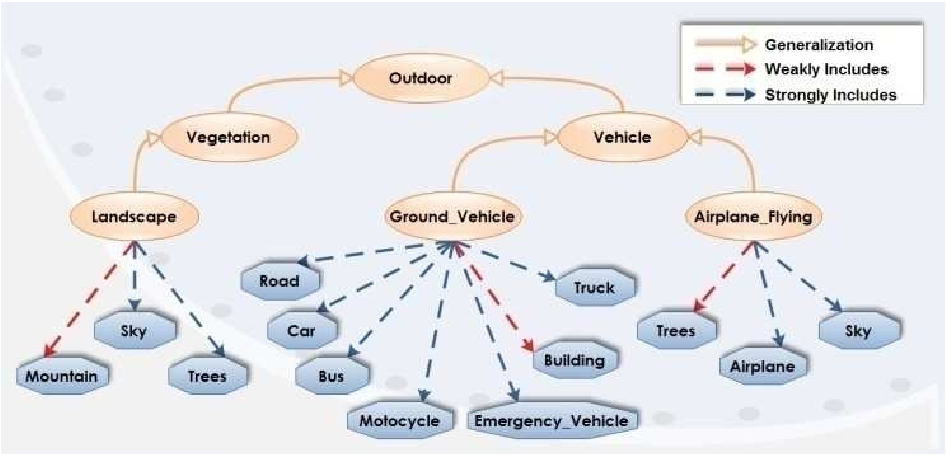
\includegraphics[scale=0.5]{graphics/c1/of}
	\end{exampleblock}
\end{frame}

\begin{frame}
	\frametitle{$C_{1}$: Obtained results with $O^{f}$}
	\centering
	\tiny
		\begin{tabular}{l||ccc|ccc|cc}\hline
				\multirow{2}{*}{\textit{\textbf{Semantic Concepts}}} & 	
				\multicolumn{3}{c}{\textbf{Concept Detector}} & 
				\multicolumn{3}{c}{\textbf{LSCOM}}&
				\multicolumn{2}{c}{\textbf{\alert{$O^{f}$}}}\\ 

				& infAP & P & R & infAP & P & R & P & R\\
				\hline
				\hline
	
				Outdoor	&-&0.52&0.59&-&	\textbf{0.88}& \textbf{0.77} & \textbf{\alert{0.9}} & \textbf{\alert{0.82}}\\
				Vegetation& 0.1 & 0.74& 0.68& 0.1& 0.74 & 0.68 & \textbf{\alert{0.93}} & \textbf{\alert{0.87}} \\
				Landscape& -& 0.6& 0.79& -& 0.6 & 0.79& \textbf{\alert{0.7}} & \textbf{\alert{0.82}}\\
				Sky& -& 0.66& 0.9& -& 0.66& 0.9 & \textbf{\alert{0.85}} & \textbf{\alert{0.95}} \\
				Trees& -& 0.62& 0.72 & - & 0.62 & 0.72 & \textbf{\alert{0.73}} & \textbf{\alert{0.82}}\\
				Mountain& -& 0.68 & 0.8 & -  & 0.68 & 0.8 & \textbf{\alert{0.83}} & \textbf{\alert{0.85}} \\
				Ground\_Vehicle& 0.043  & 0.3& 0.66& \textbf{0.18} & \textbf{0.6} & \textbf{0.73} 
								& \textbf{\alert{0.69}}&\textbf{\alert{0.75}}\\
				Road& -& 0.43& 0.6 & -& 0.43& 0.6 & \textbf{\alert{0.88}} & \textbf{\alert{0.9}} \\
				Car  & 0.075 & 0.42 & 0.64& \textbf{0.17} & \textbf{0.58} & \textbf{0.73} 
								& \textbf{\alert{0.79}} & \textbf{\alert{0.83}}\\
				Bus& -& 0.52& 0.73& - & 0.52& 0.73 &0.52 & 0.73\\
				Bicycles& 0.142& 0.67& 0.92& \textbf{0.185}& \textbf{0.82}& \textbf{0.97} & \textbf{\alert{0.83}} & 0.97\\
				Emergency Vehicle& -& 0.9& 0.83& - & 0.9& 0.83 & 0.9& 0.83\\
				Building& 0.022& 0.18& 0.22& \textbf{0.1}& \textbf{0.5}& \textbf{0.43} & \textbf{\alert{0.55}} & \textbf{\alert{0.45}} \\
				Truck & -& 0.35& 0.37& -& 0.35& 0.37 & 0.35 & 0.37\\
				Airplane Flying & 0.102& 0.8 & 0.78& 0.102& 0.8& 0.78 & \textbf{\alert{0.83}} & \textbf{\alert{0.79}}  \\
				Airplane  & -& 0.5& 0.6& -& \textbf{0.6}& 0.6  & \textbf{\alert{0.71}} & \textbf{\alert{0.69}}\\
				\hline
		\end{tabular}
		%\pause
		\footnotesize
		\begin{exampleblock}{}
			Semantic Enhancement of about \alert{$21\%$} compared to a classical concept detection.
		\end{exampleblock}
\end{frame}

\begin{frame}
	\frametitle{$C_{1}$: Related publications}
	\begin{block}{}
		{\tiny
		\begin{itemize}
			\item \citep{Elleuch2010} Elleuch, N., \textbf{Zarka, M.}, Feki, I., Ammar, A. B., 
				\&{} Alimi, A. M. (2010). REGIMVID at TRECVID2010: semantic 
				indexing. In P. Over et al. (Eds.), \emph{TRECVID 2010 workshop
				participants notebook papers, Gaithersburg, MD, USA, november 2010}. 
				National Institute of Standards and Technology (\alert{NIST}). 
				
			\item \citep{Zarka2011a} \textbf{Zarka, M.}, Ammar, A. B., \&{} Alimi, A. M. (2011). 
				Multimodal fuzzy fusion system for semantic video indexing. 
				In \emph{IEEE symposium on computational intelligence for multimedia,
				signal and vision processing, CIMSIVP 2011, Paris, France} (pp. 60--66). \alert{IEEE}.

			\item \citep{Elleuch2011} Elleuch, N., \textbf{Zarka, M.}, Ammar, A. B., \&{} Alimi, A. M. (2011). 
				A fuzzy ontology: Based framework for reasoning in visual video content analysis 
				and indexing. In Proceedings of the eleventh international 
				workshop on multimedia data mining (pp. 1--8). New York, NY, USA: \alert{ACM}.
				

			\item \citep{Ksentini2012} Ksentini, N., \textbf{Zarka, M.}, Ammar, A. B., \&{} Alimi, A. M. (2012). 
				Toward an assisted context based collaborative annotation. In P. Lambert (Ed.), 
				\emph{10th international workshop on content-based multimedia indexing, 
				CBMI 2012, annecy, france, june 27--29, 2012} (pp. 71--76). \alert{IEEE}.
				
		\end{itemize}
		}
	\end{block}	
\end{frame}

		\subsection[$C_{2}$ Fuzzy reasoning framework to improve semantic video Indexing]
				{$C_{2}$ Fuzzy reasoning framework to improve semantic video Indexing}
			\begin{frame}
	\frametitle{$C_{2}$: Fuzzy Reasoning Framework for Video Indexing}
	 {\small
	\begin{itemize}
	 
% 	  \item $C_{2}$ : An \alert{automated} framework to \alert{construct} an ontology,
 	  \item Ontology Management: \textbf{\alert{Knowledge Extraction}}, 
 	  \textbf{\alert{Ontology Structure}}, \textbf{\alert{Reasoning}} and \textbf{\alert{Evolving}}.
	\end{itemize}
	}
	\begin{center}\hspace*{-1cm} 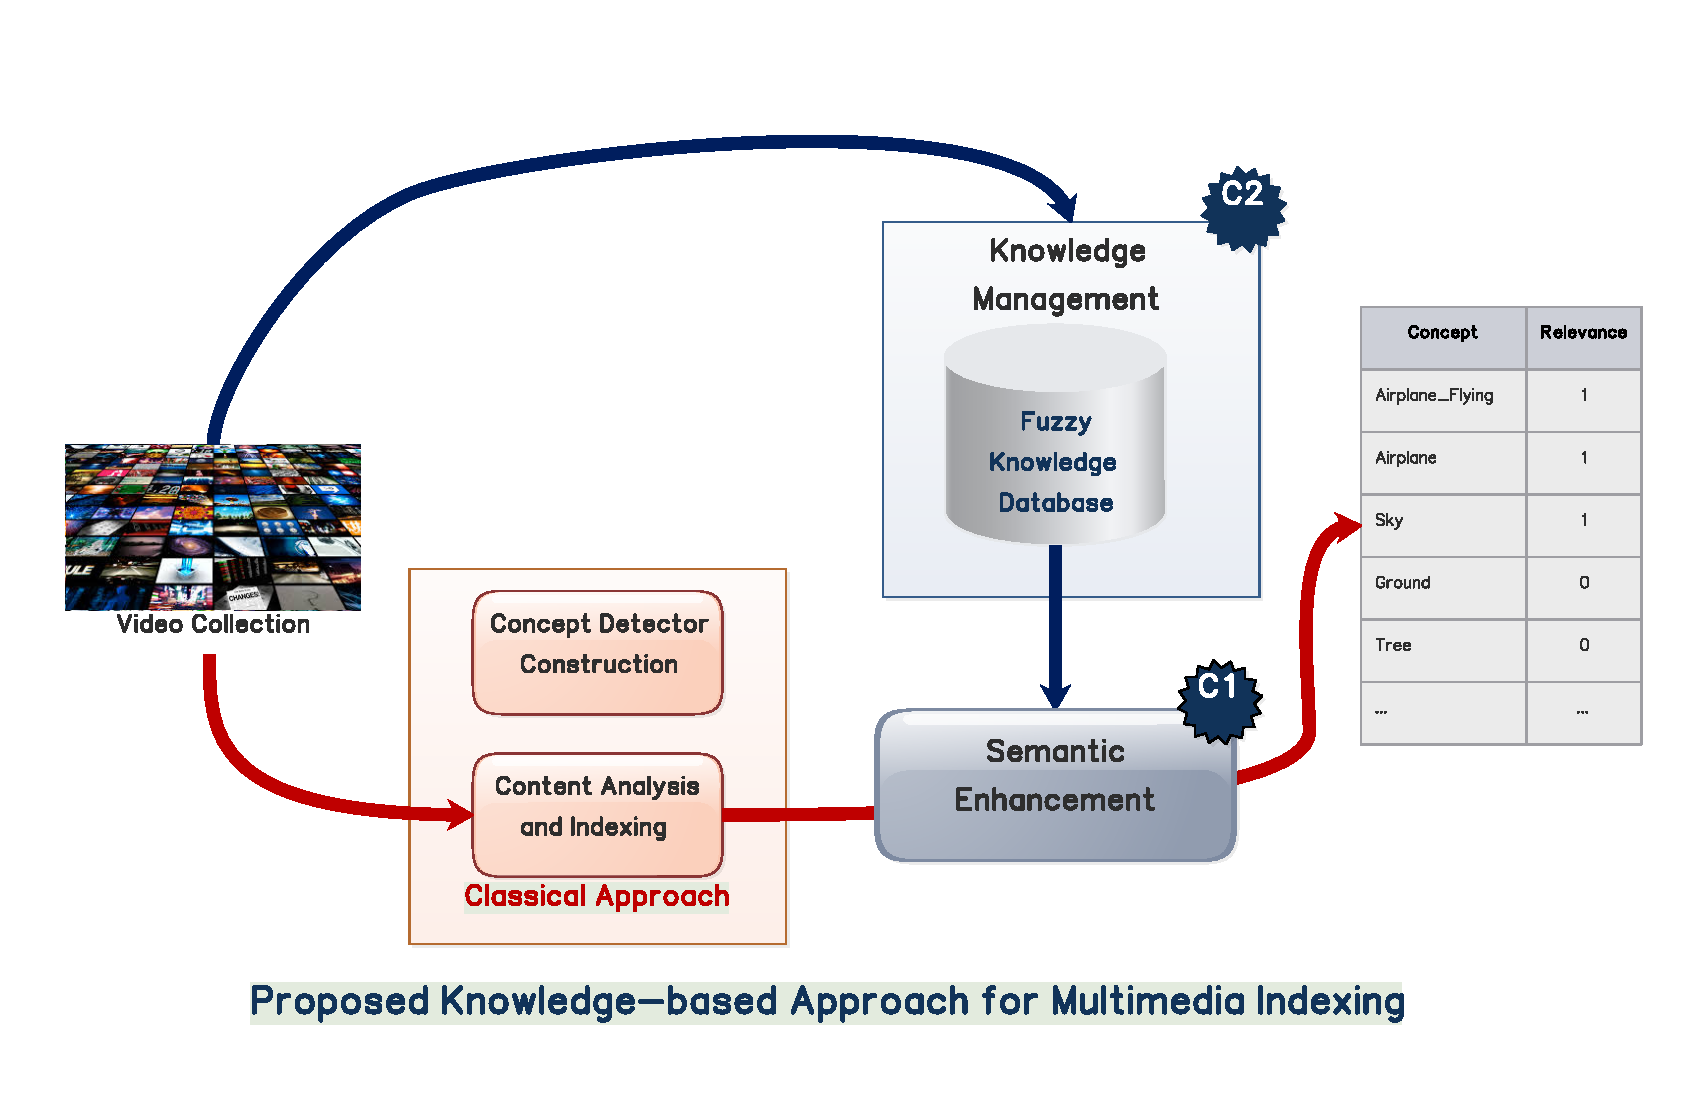
\includegraphics[scale=0.30]{graphics/contribution/contrib_overview_3} \end{center}

\end{frame}

\begin{frame}
	\frametitle{$C_{2}$: Proposed Approach - Inputs}
	\begin{block}{}
	 \begin{itemize}
	  \item \alert{Annotated} Multimedia Content,
	  \item A \alert{content} with a set of detected semantic \alert{concepts}.
	 \end{itemize}
	\end{block}

	{\hspace*{-1cm}\centering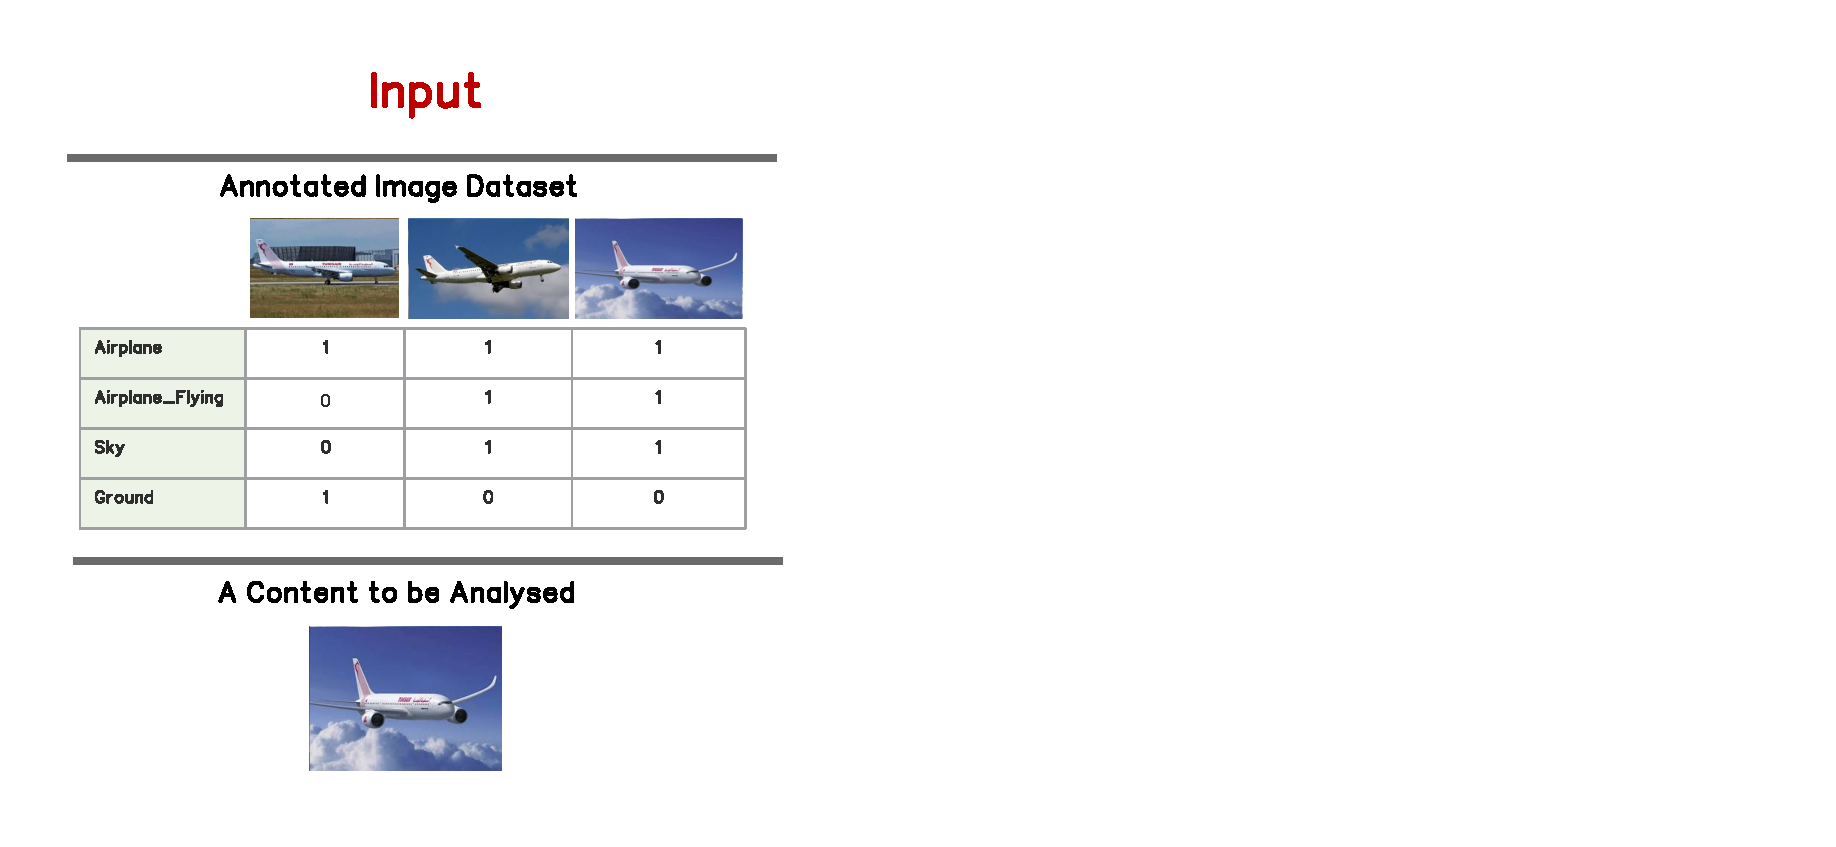
\includegraphics[scale=0.4]{graphics/c2/main_c2_1}}
\end{frame}

\begin{frame}
	\frametitle{$C_{2}$: Proposed Approach - Knowledge Extraction}
	\begin{block}{}
	 \begin{itemize}
	  \item Each \alert{concept} is considered as a Vector,
	  \item Computing \alert{similarities} between concepts for a given context.
	 \end{itemize}
	\end{block}
	{\hspace*{-1cm}\centering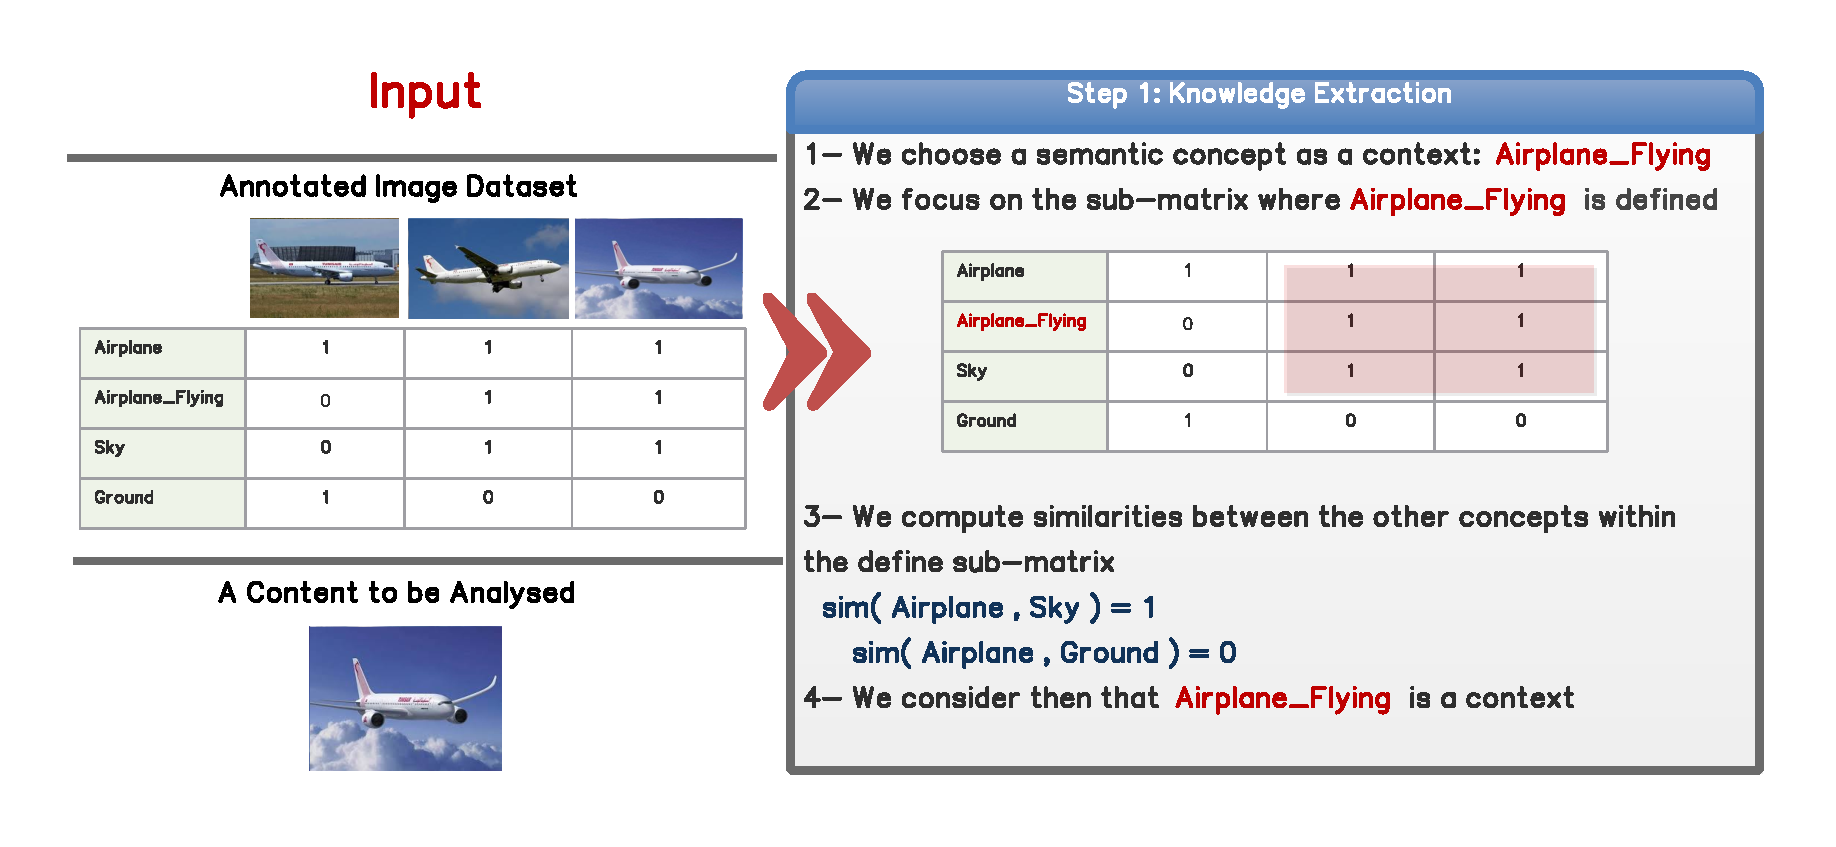
\includegraphics[scale=0.4]{graphics/c2/main_c2_2}}
\end{frame}

\begin{frame}
	\frametitle{$C_{2}$: Proposed Approach - Ontology Structure}
	\begin{block}{}
	 \begin{itemize}
	  \item \alert{Context based} ontology structure,
	  \item Computed \alert{relationships} are populated within the ontology.
	 \end{itemize}
	\end{block}
	\only<1>{\hspace*{-1cm}\centering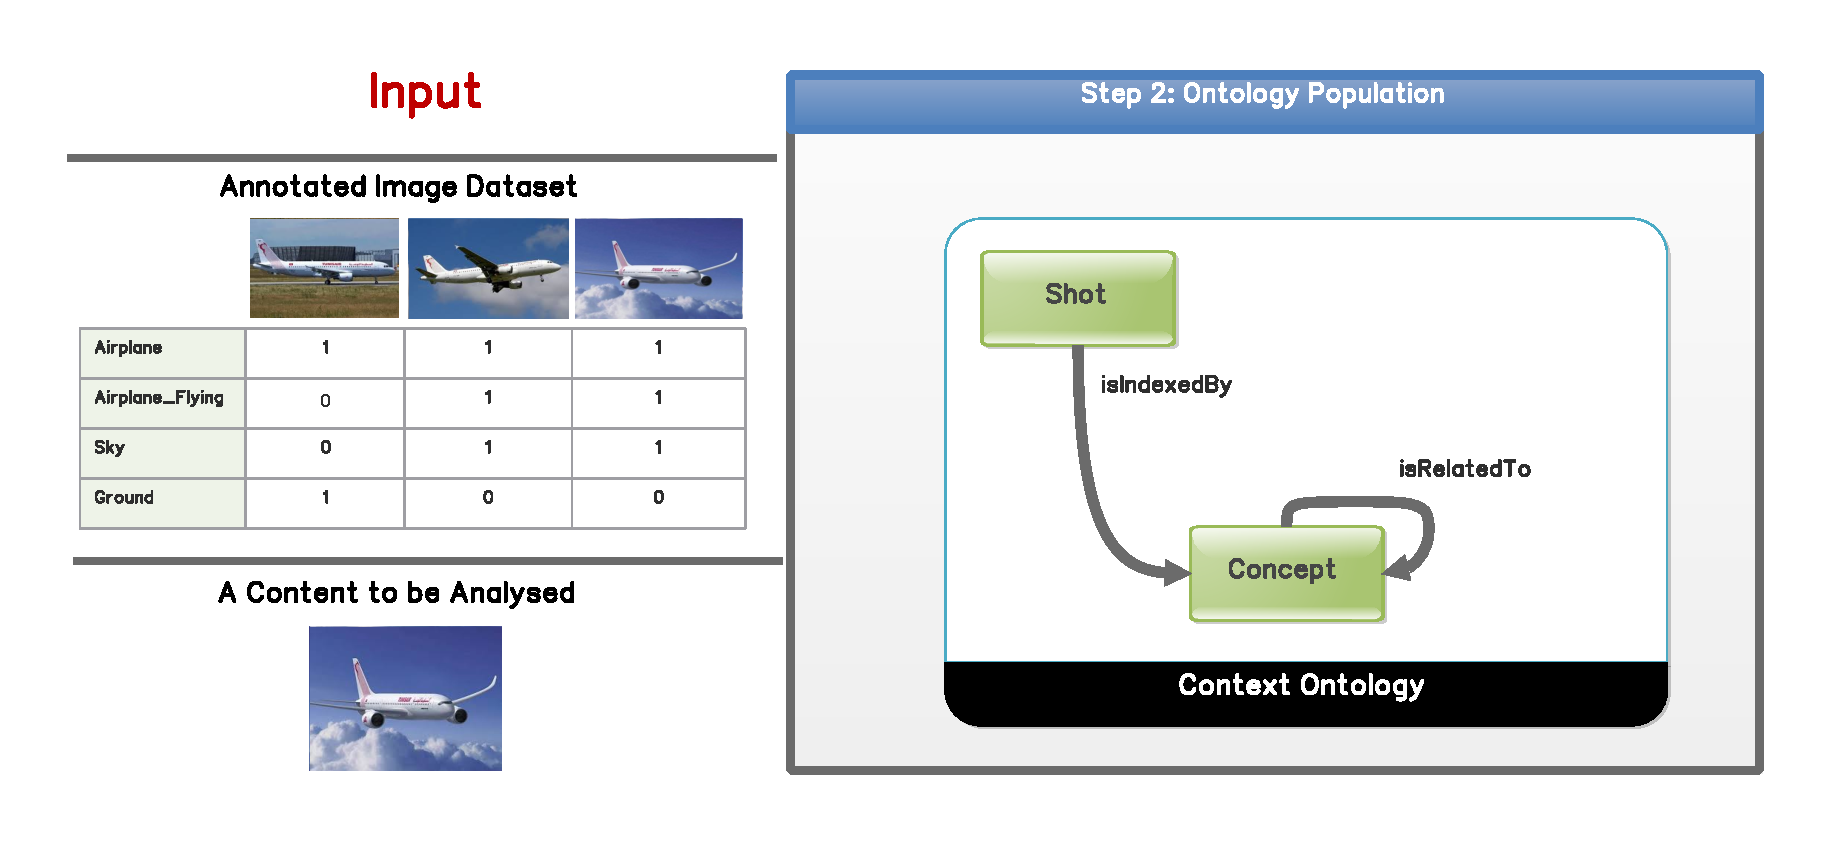
\includegraphics[scale=0.4]{graphics/c2/main_c2_3_1}}
	\only<2>{\hspace*{-1cm}\centering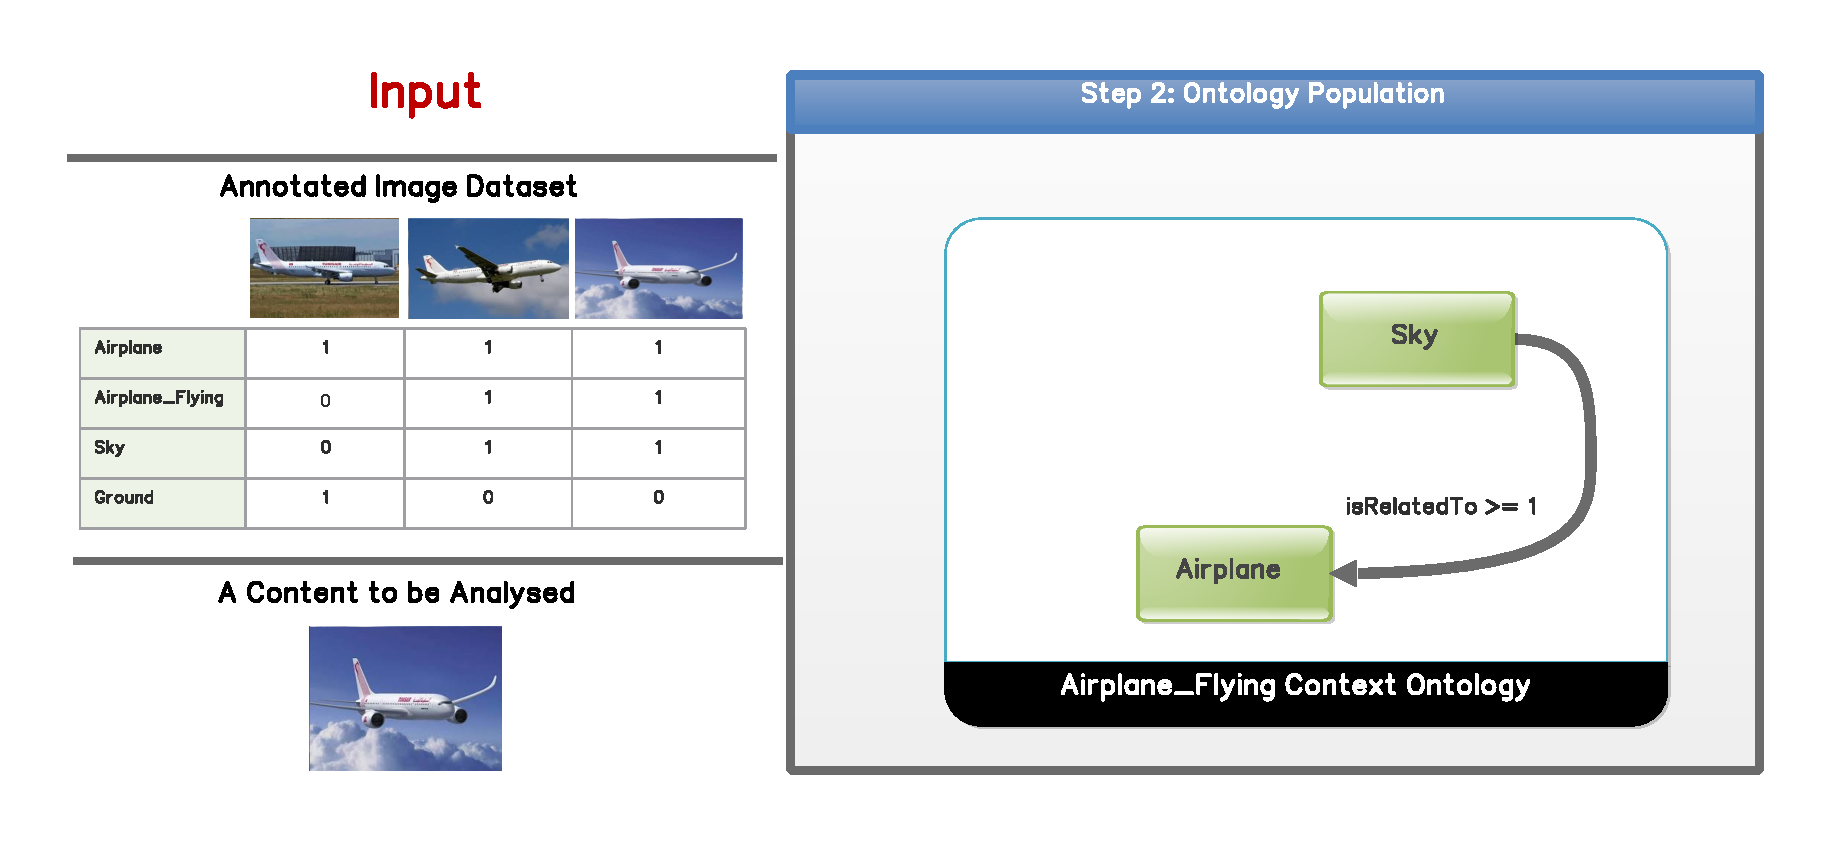
\includegraphics[scale=0.4]{graphics/c2/main_c2_3_2}}
\end{frame}

\begin{frame}
	\frametitle{$C_{2}$: Proposed Approach - Ontology Reasoning}
	\begin{block}{}
	 \begin{itemize}
	  \item Reasoning based on interpreting the \alert{$isIndexedBy$} roles,
	  \item We used \alert{\textit{``tableau''}} reasoning algorithm \tiny{\citep{Horrocks2005}}.
	 \end{itemize}
	\end{block}
	{\hspace*{-1cm}\centering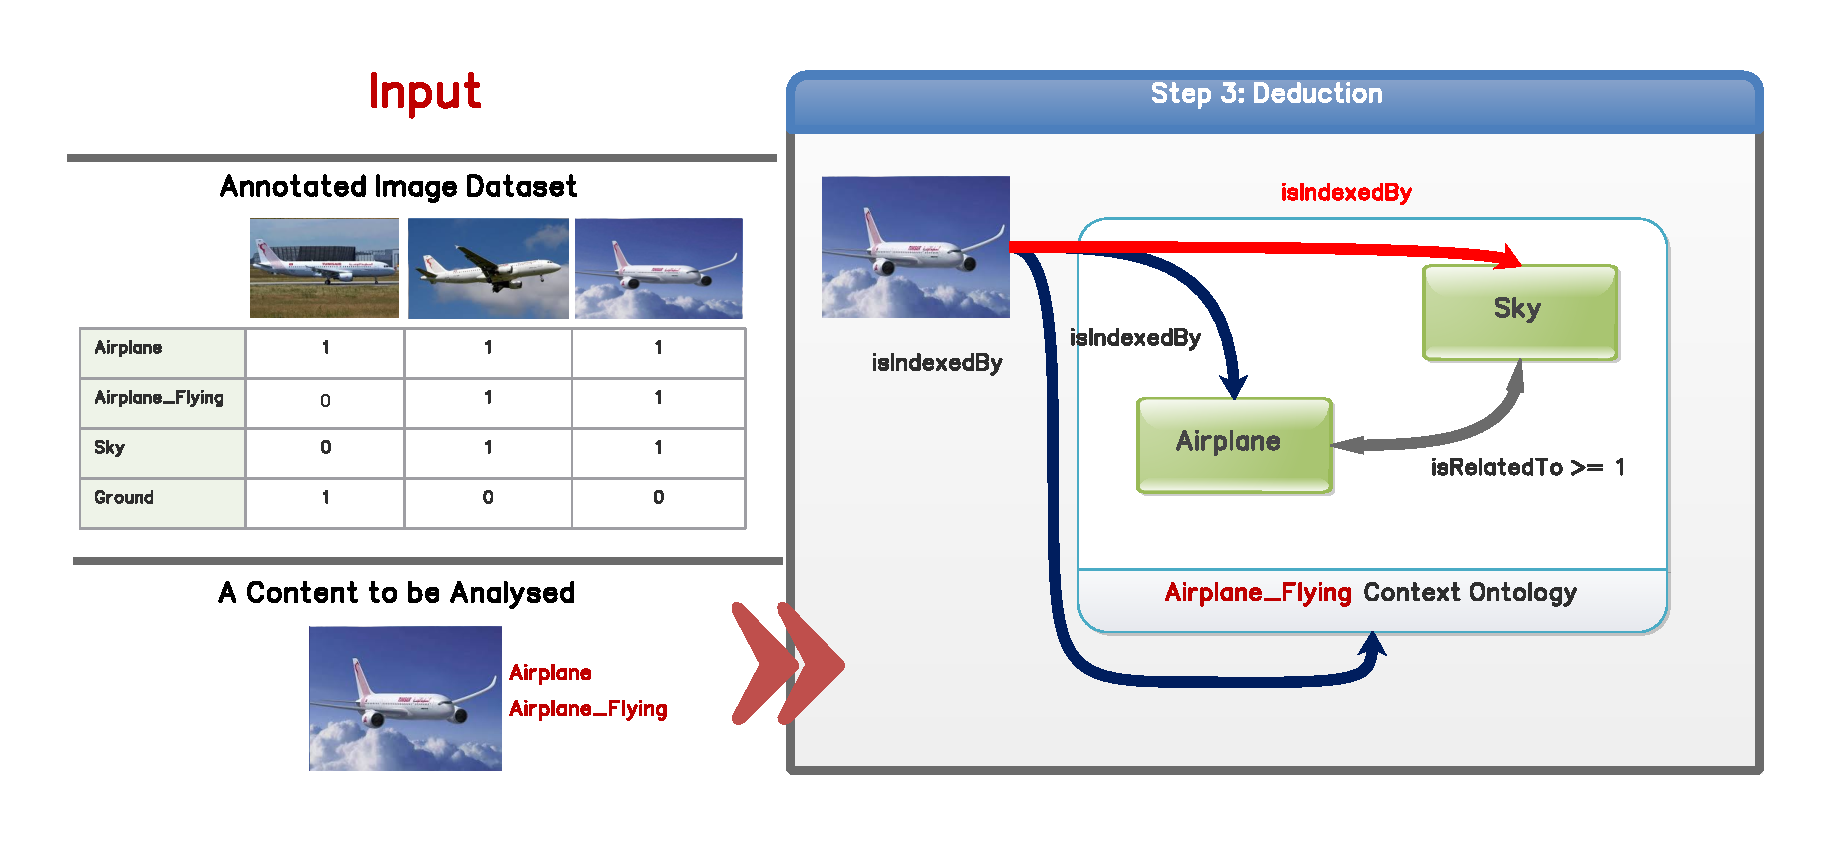
\includegraphics[scale=0.4]{graphics/c2/main_c2_4}}
\end{frame}

\begin{frame}
	\frametitle{$C_{2}$: Proposed Approach - Ontology Evolution}
	\begin{block}{}
	 \begin{itemize}
	  \item \alert{Updating} the ontology content,
	  \item The ontology evolution is based on \alert{experts} analysis.
	 \end{itemize}
	\end{block}
	{\hspace*{-1cm}\centering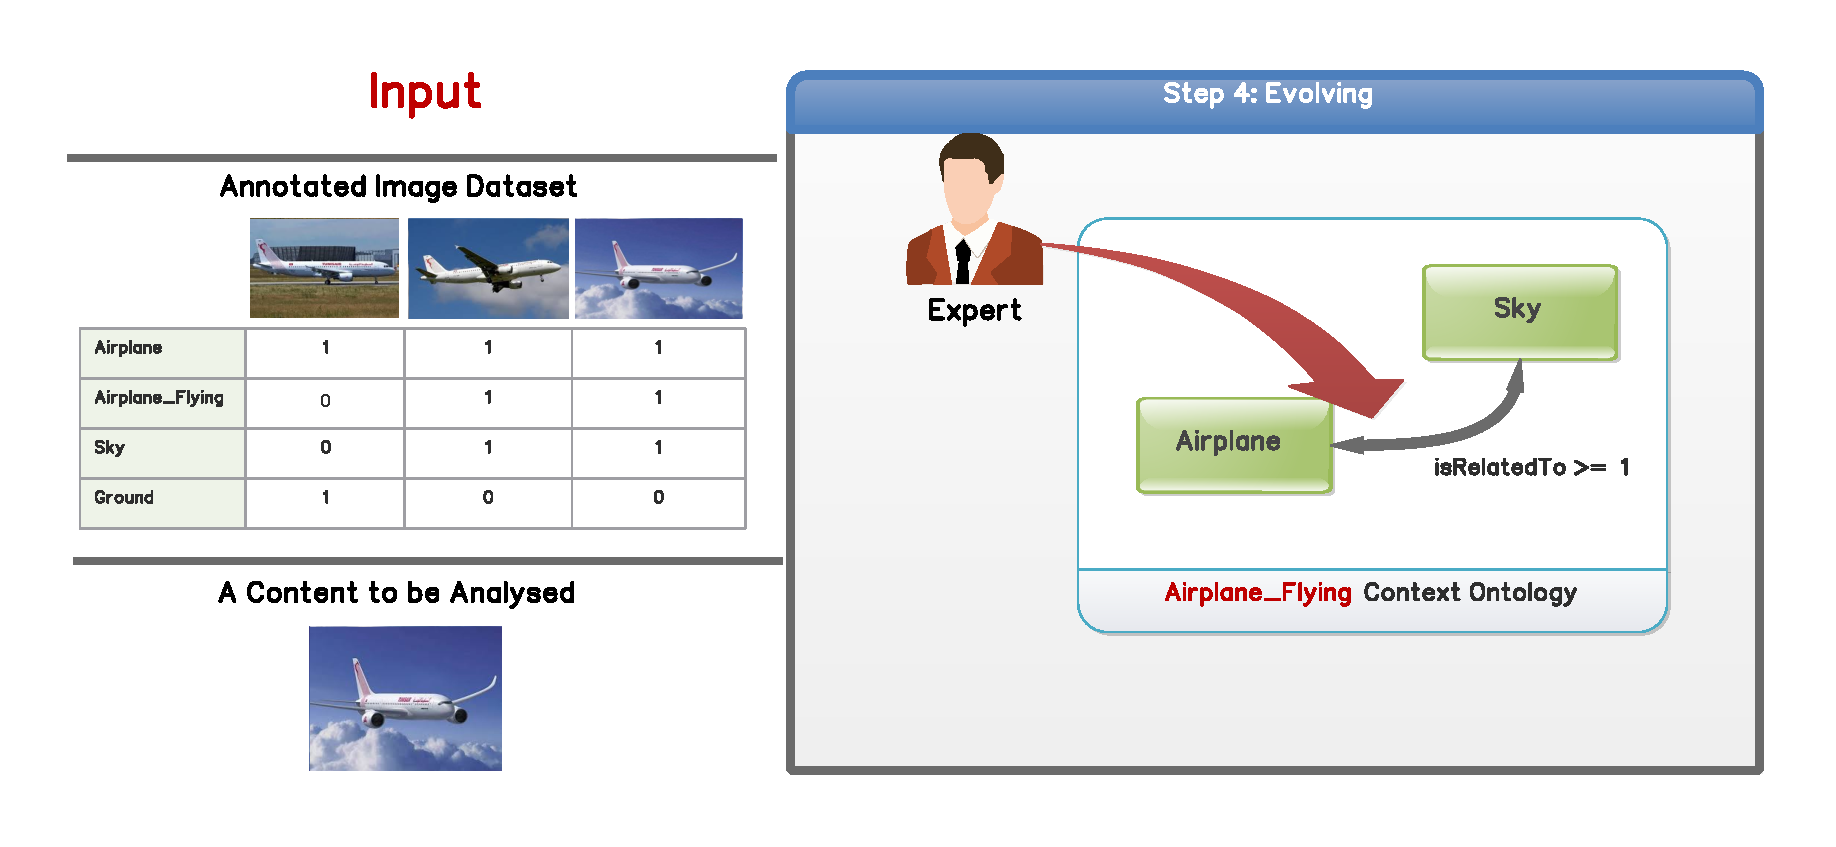
\includegraphics[scale=0.4]{graphics/c2/main_c2_5}}
\end{frame}


\begin{frame}
	\frametitle{$C_{2}$: Experiments - Setup}
	\begin{exampleblock}{Experimentation Setup}
		{\small
		\begin{itemize}		
			\item \textsc{ImageClef 2012}
			\item Photo dataset : \alert{\textbf{25.000}} images (\textbf{15.000} images for training 
				and \textbf{10.000} images for test)
			\item  \alert{94} semantic concepts
		\end{itemize}
		}
	\end{exampleblock}

	\begin{exampleblock}{Baseline}
		{\small
		\begin{itemize}
			\item We look to evaluate the semantic enhancement of a non knowledge-based approach 
			    \alert{\citep{Ksibi2012}},
			\item \alert{Visual} semantic indexing,
			\item We used the constructed \alert{contextual Ontologies}
		 \end{itemize}
		}
	\end{exampleblock}
\end{frame}

\begin{frame}
	\frametitle{$C_{2}$: Experiments - Ontologies construction}
	\begin{exampleblock}{Distribution of extracted $\mathsf{isRelatedTo}$ roles}
		 \centering \tiny
		\begin{tabular}{c l c c c c c c c c c c} \hline
		~&\textbf{Context}& $[0, 0.3[$ & $[0.3, 0.5[$ & $[0.5, 0.7[$ & $[0.7, 1.0]$ \\ 
		\hline
			1&sentiment\_euphoric	&783	&605	&510	&534\\
			2&sentiment\_happy		&2020	&864	&519	&444\\
			3&setting\_sportsrecreation&1264	&752	&483	&456\\ 
			4&age\_child		&1045	&649	&493	&441\\ 
			5&relation\_familyfriends	&1150	&903	&398	&522\\ \hline
			86&fauna\_cat	&115	&105	&91	&203\\ 
			87&fauna\_insect		&107	&63	&43	&192\\
			88&fauna\_rodent		&43	&53	&43	&139\\ 
			89&fauna\_amphibianreptile	&24	&29	&43	&127\\ 
			90&fauna\_spider	&3	&20	&16	&48\\ \hline 
			\multicolumn{2}{c}{\textbf{All contexts}}	&91803 	&50210	&27435	&33667\\
			\hline
			\multicolumn{2}{c}{\textbf{Total}}& \multicolumn{10}{c}{\textbf{\alert{203 115} $\mathsf{isRelatedTo}$ 
								roles for 90 defined contexts}}\\ \hline
		\end{tabular}
		
	\end{exampleblock}	
	%\pause
	%\begin{exampleblock}{}
	{\tiny \centering
	\begin{equation*}
			\begin{array}{ c c l c l}
			age\_adult & - &\mathcal{K}^{f}_{age\_adult} 
				& - & (age\_teenager,sentiment\_scary):\mathsf{isRelatedTo} \geq 0.12\\
			transport\_car & - &\mathcal{K}^{f}_{transport\_car}
				& - & (sentiment\_happy,timeofday\_day):\mathsf{isRelatedTo} \geq 0.95\\
			setting\_homelife & - &\mathcal{K}^{f}_{setting\_homelife} 
				& - & (quantity\_biggroup,sentiment\_happy):\mathsf{isRelatedTo} \geq 0.81\\
			\end{array}
	\end{equation*}
	}
	%\end{exampleblock}
		
\end{frame}


\begin{frame}
	\frametitle{$C_{2}$: Experiments - Obtained Results}
	\begin{exampleblock}{Enhancement Assessment}
		{\small \centering{
			\begin{tabular}{l||cc|cc} 
			
			  & \multicolumn{2}{c}{\textbf{\textit{map$_{i}$}}} 
			  &\multicolumn{2}{c}{\textbf{\textit{gmap$_{i}$}}}  \\
			  
			  & value & \% & value & \%  \\
			\hline  \hline  
		
			Our proposed framework & 
						$0,1324$ & \textbf{\alert{5.08}} & 		
						$0,0808$ & \textbf{\alert{3.46}} \\ 
			\citep{Ksibi2012}  &  $0.126$ & - & $0.078$ & -  \\
			\hline 
			\end{tabular}
		}}
	\end{exampleblock}	
	
	\begin{exampleblock}{Ontology evolution}
	{\footnotesize
		\begin{itemize}
			\item \alert{$3$} experts,
			\item Up to \alert{$0.54 \%$} of semantic enhancement.
		\end{itemize}
	}
	\end{exampleblock}
\end{frame}

\begin{frame}
	\frametitle{$C_{2}$: Related publication}
	\begin{block}{}
		\begin{itemize}
			\item \citep{Zarka2015} \textbf{Zarka, M.}, Ben Ammar, A., \&{} Alimi, A. (2016). 
				Fuzzy reasoning framework to improve semantic video interpretation. 
				\emph{Multimedia Tools and Applications}, 5719--5750.
		\end{itemize}
	\end{block}
\end{frame}


		\subsection[$C_{3}$ Scalable Ontology-Driven Approach for Concept Detector]
				{$C_{3}$ Scalable ontology-driven Approach to Construct Hierarchical Semantic Concept Detectors}
			\begin{frame}
	\frametitle{$C_{3}$: Scalable Ontology-based Concept Detection}
	 {\small
	\begin{itemize}
 	  \item $C_{3}$ : A Scalable Semantic \alert{Hierarchical} Framework.
 	  \end{itemize}
	}
	\begin{center}\hspace*{-1cm} 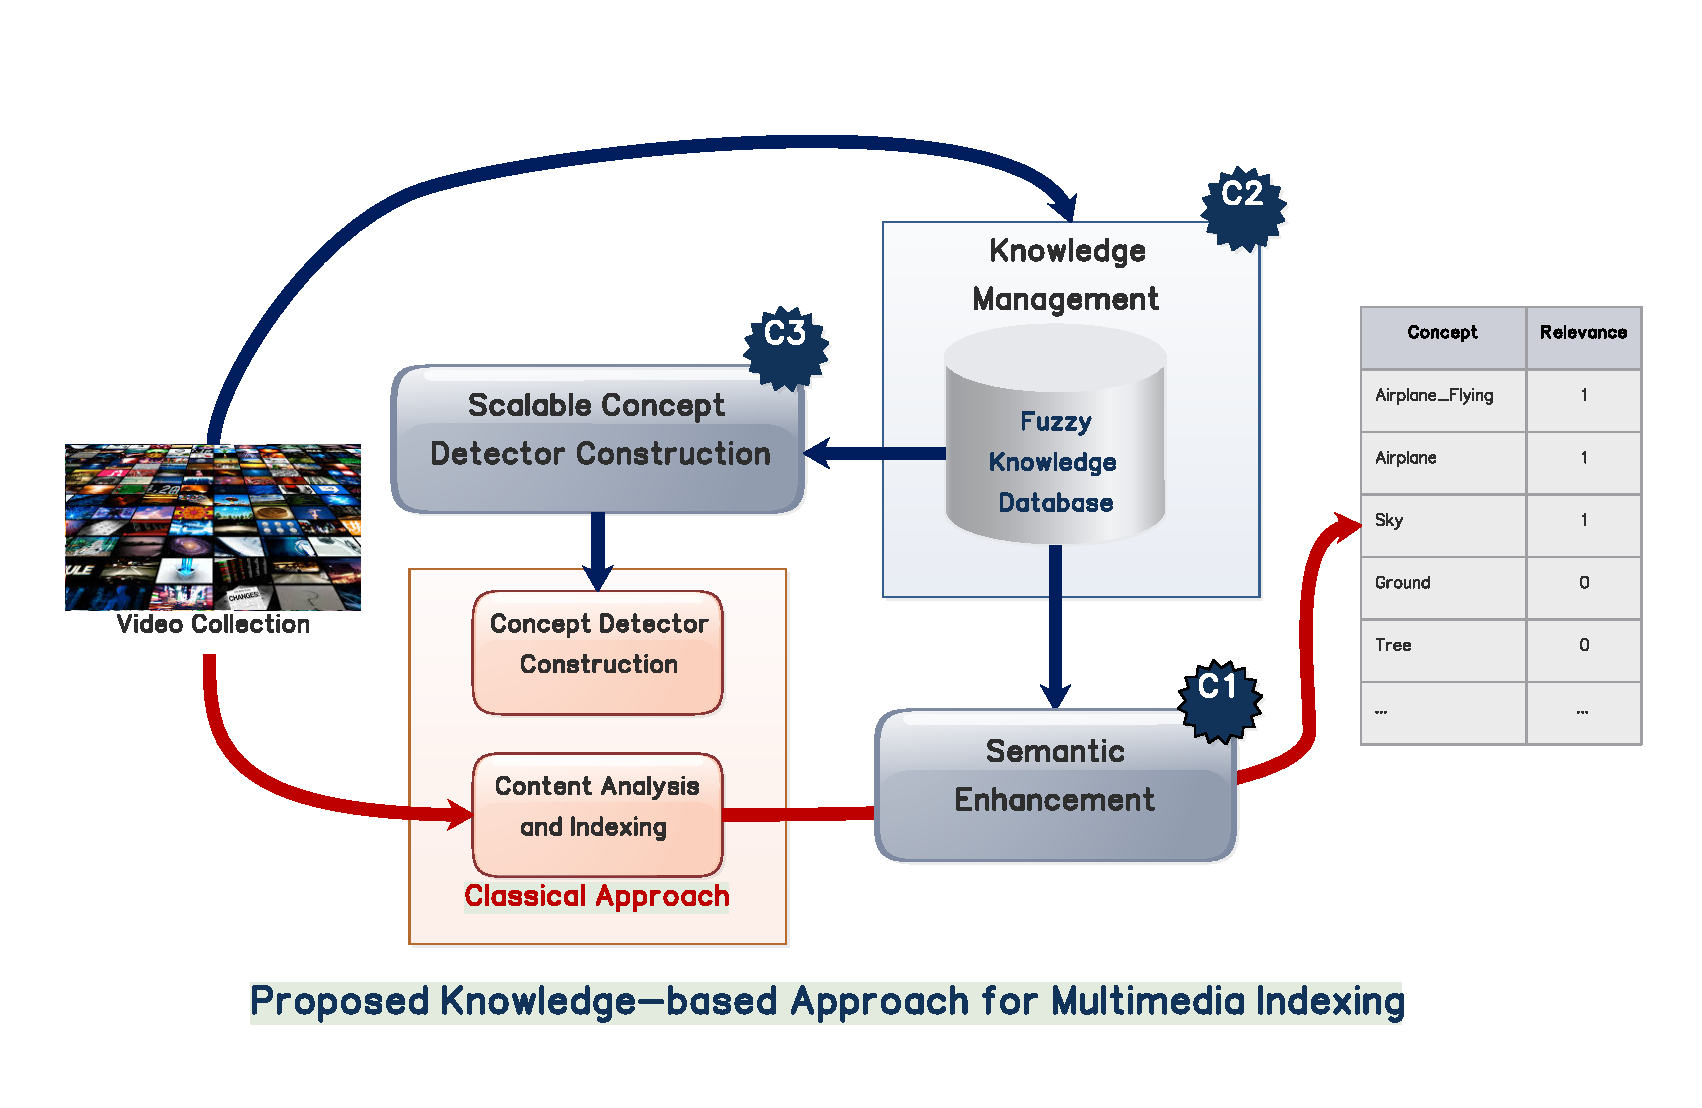
\includegraphics[scale=0.30]{graphics/contribution/contrib_overview_4} \end{center}

\end{frame}


\begin{frame}
	\frametitle{Classical Approach}
	\begin{block}{}
	 \begin{itemize}
	  \item Construct a \alert{dedicated} detector for each concept,
	  \item For a given content, all the detectors are fired.
	 \end{itemize}
	\end{block}
	\hspace*{-1cm}\centering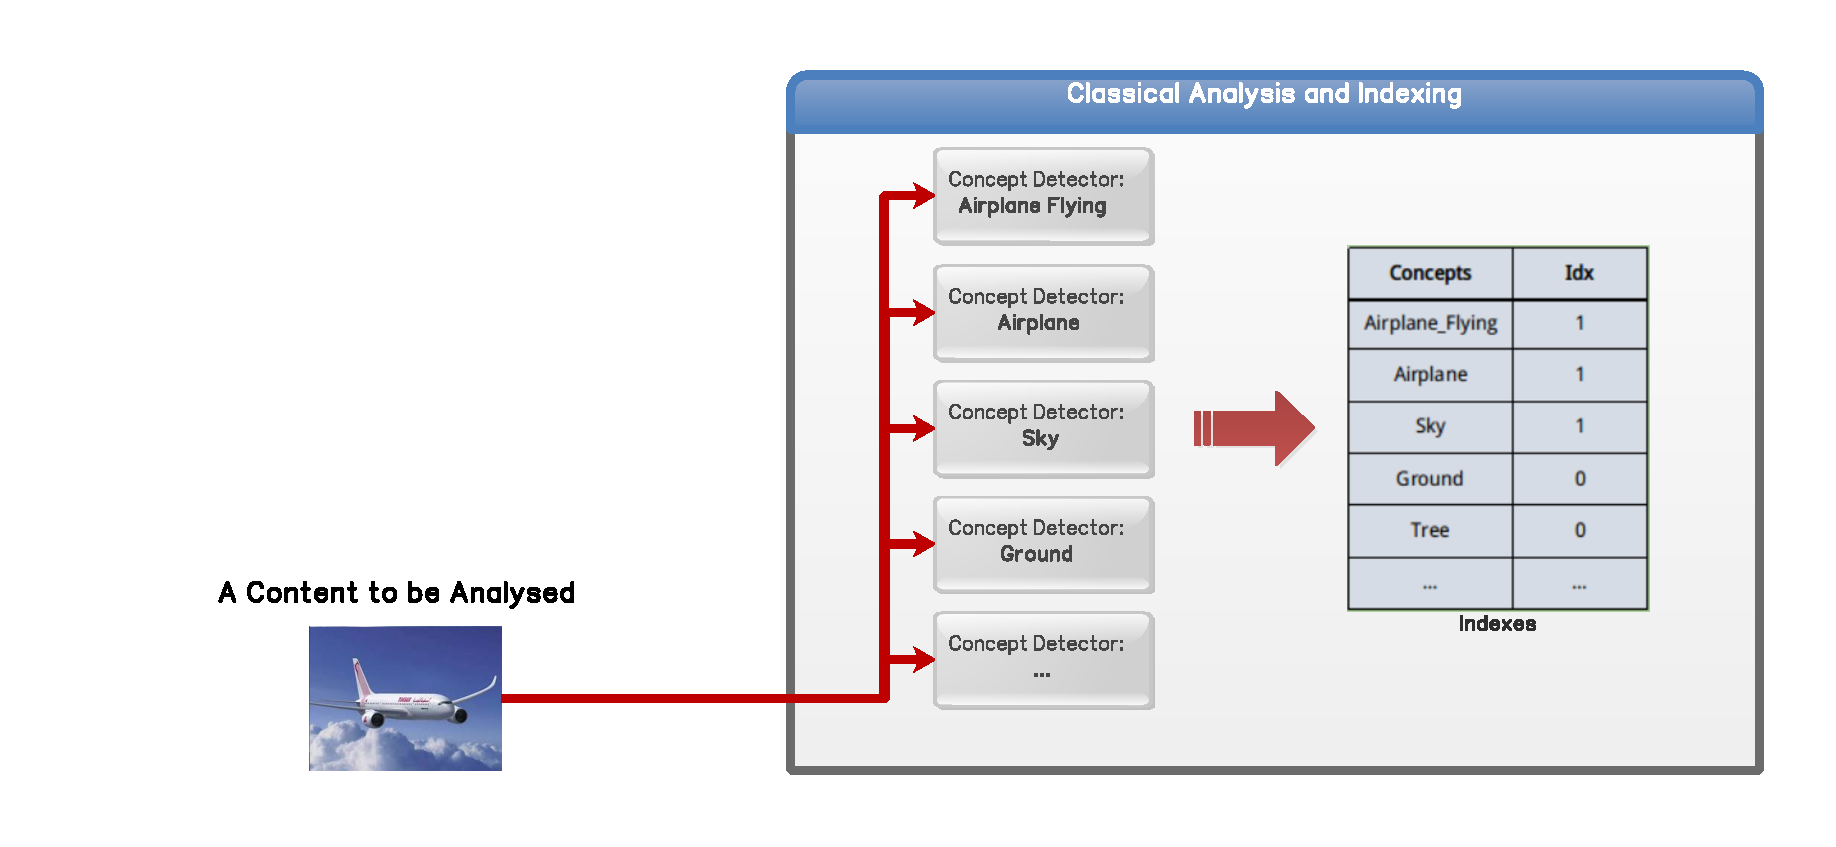
\includegraphics[scale=0.39]{graphics/c3/main_c3_1}
% 	\only<2>{\hspace*{-1cm}\centering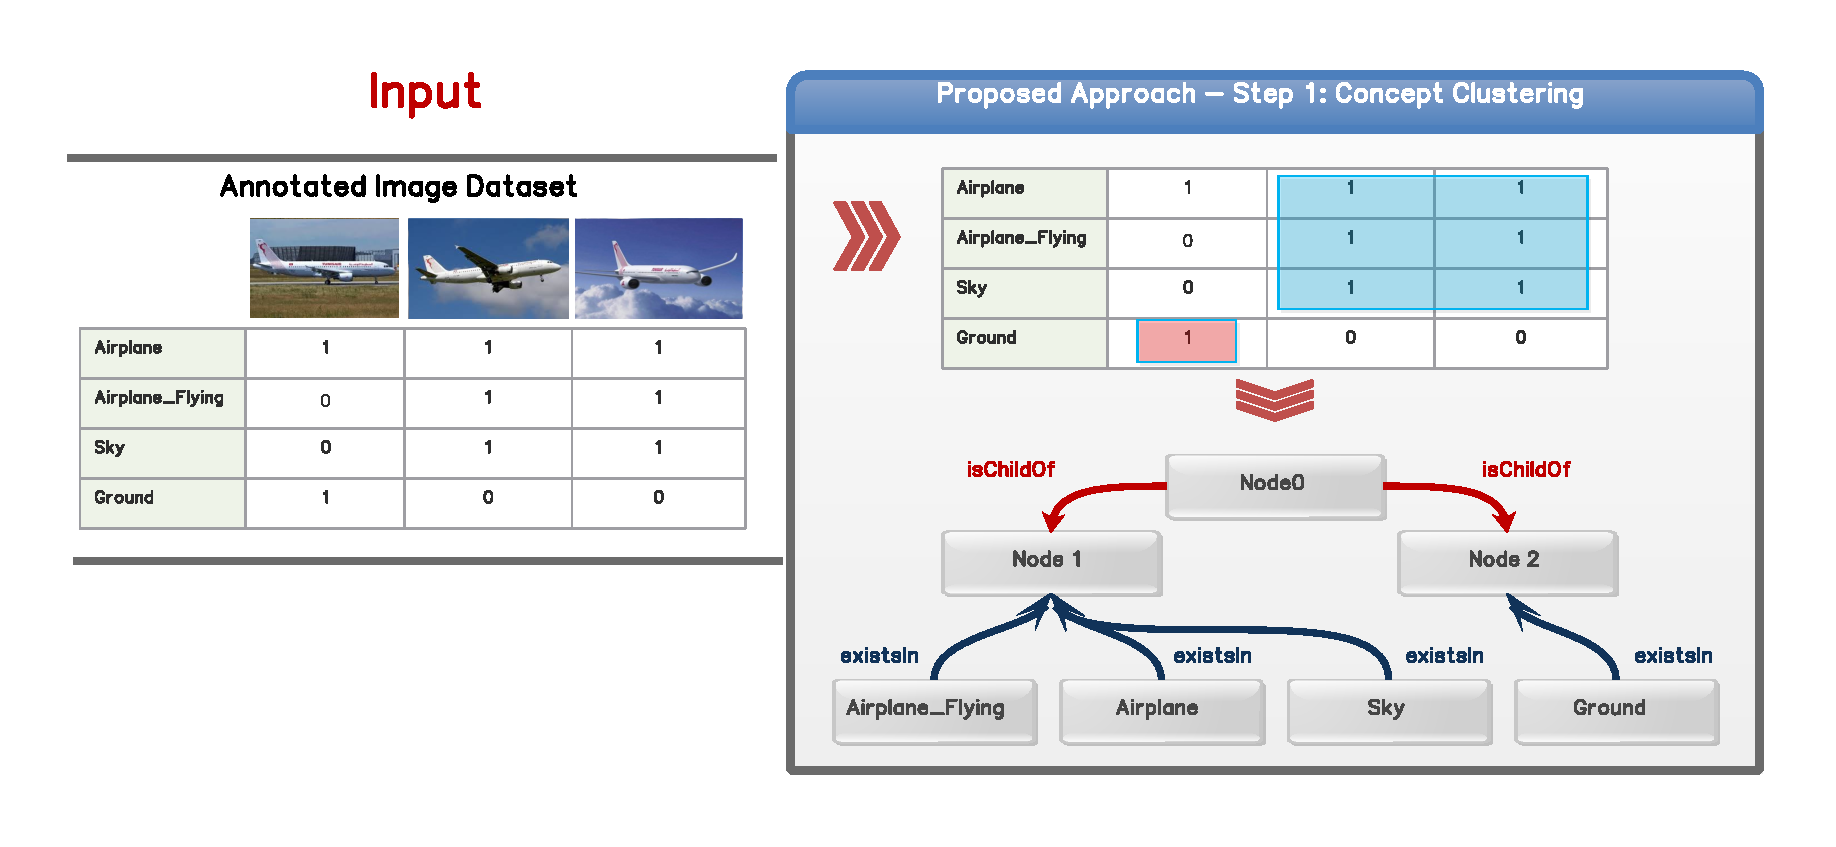
\includegraphics[scale=0.41]{graphics/c3/main_c3_2}}
% 	\only<3>{\hspace*{-1cm}\centering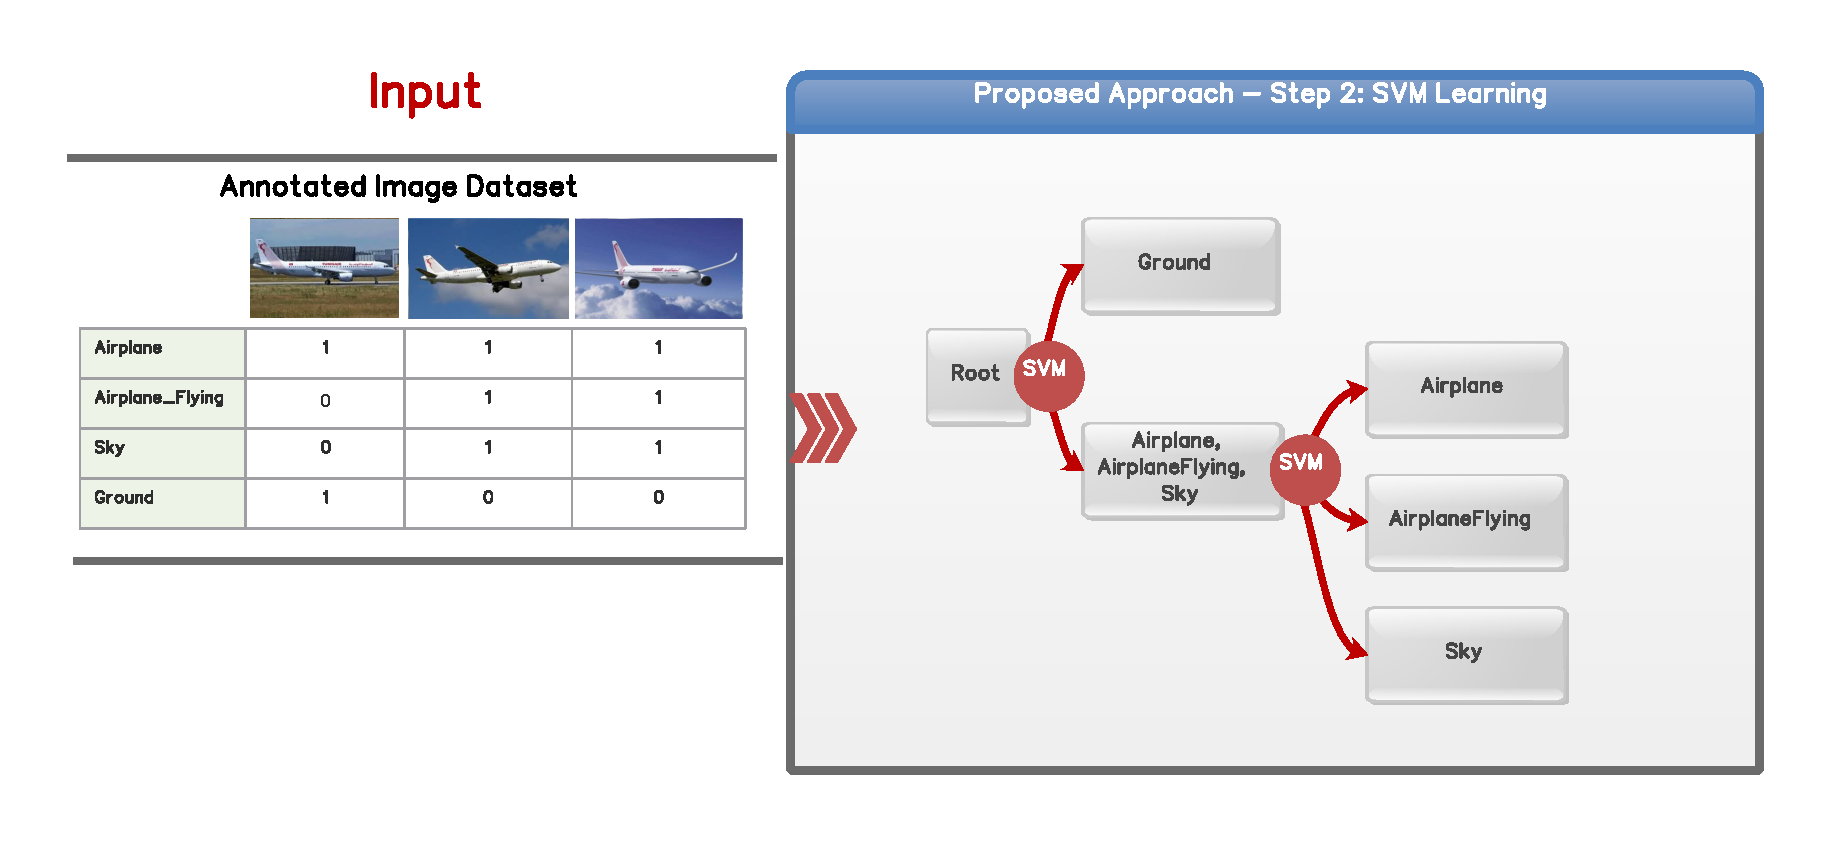
\includegraphics[scale=0.41]{graphics/c3/main_c3_3}}
% 	\only<4>{\hspace*{-1cm}\centering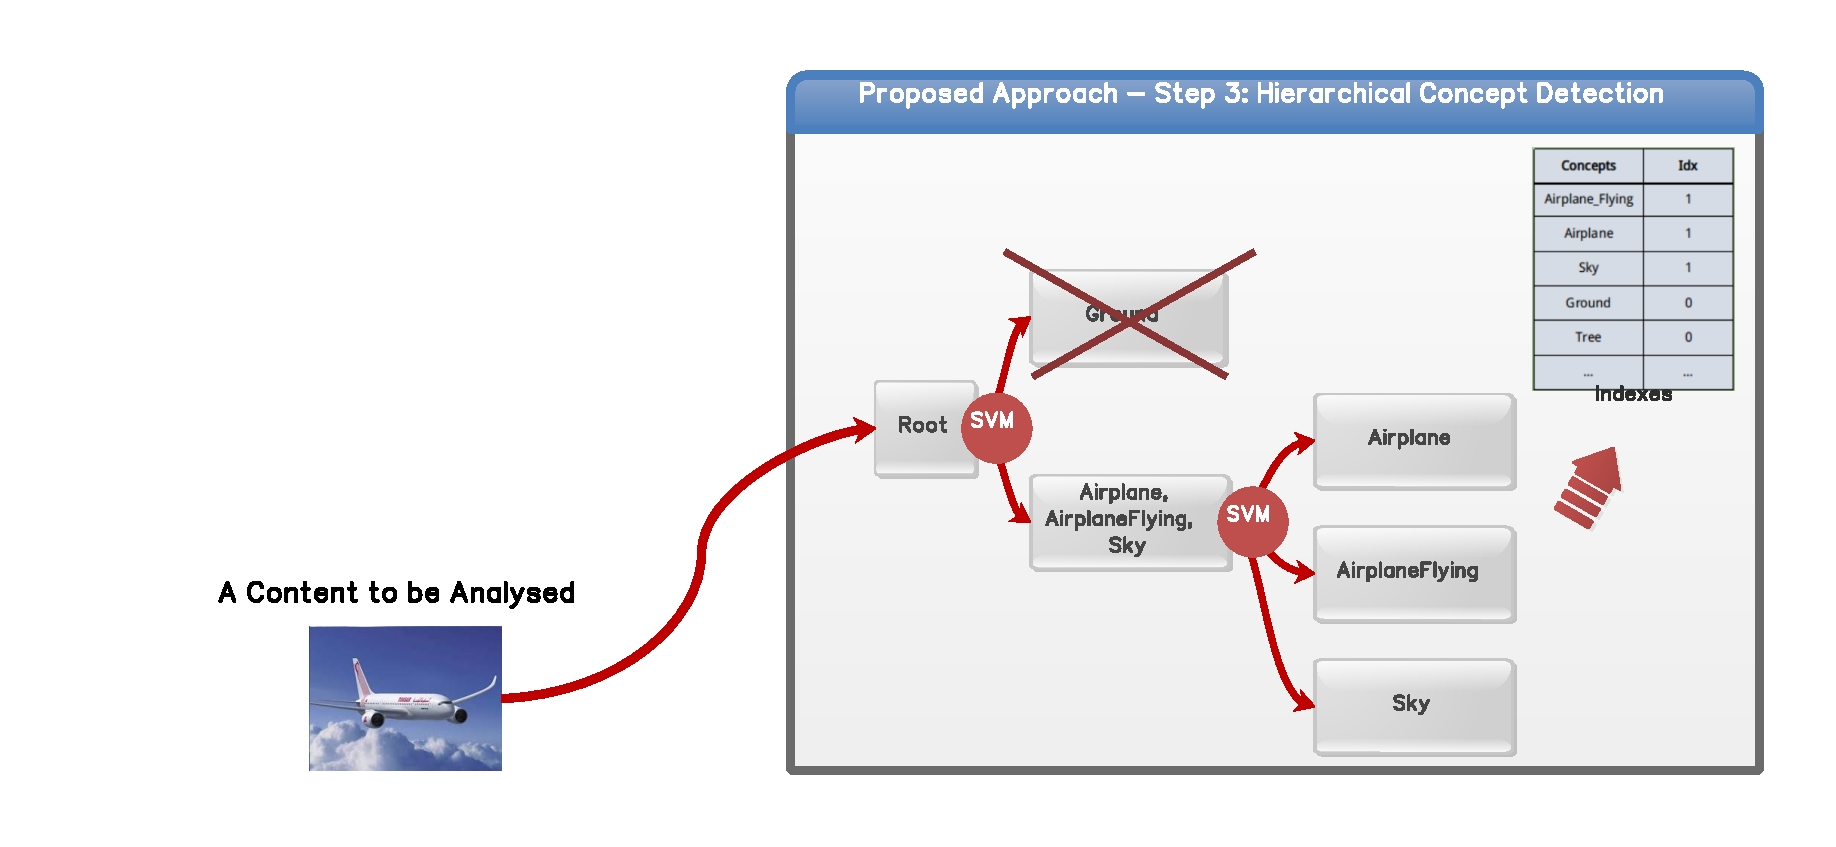
\includegraphics[scale=0.41]{graphics/c3/main_c3_4}}
\end{frame}

\begin{frame}
	\frametitle{$C_{3}$: Proposed Approach - Hierarchical Ontology Structure}
	\begin{block}{}
	 \begin{itemize}
	  \item An ontology structure based on concept \alert{hierarchy}, 
	  \item Two main roles: \textbf{isChildOf} and \textbf{existsIn}.
	 \end{itemize}
	\end{block}
	\hspace*{-1cm}\centering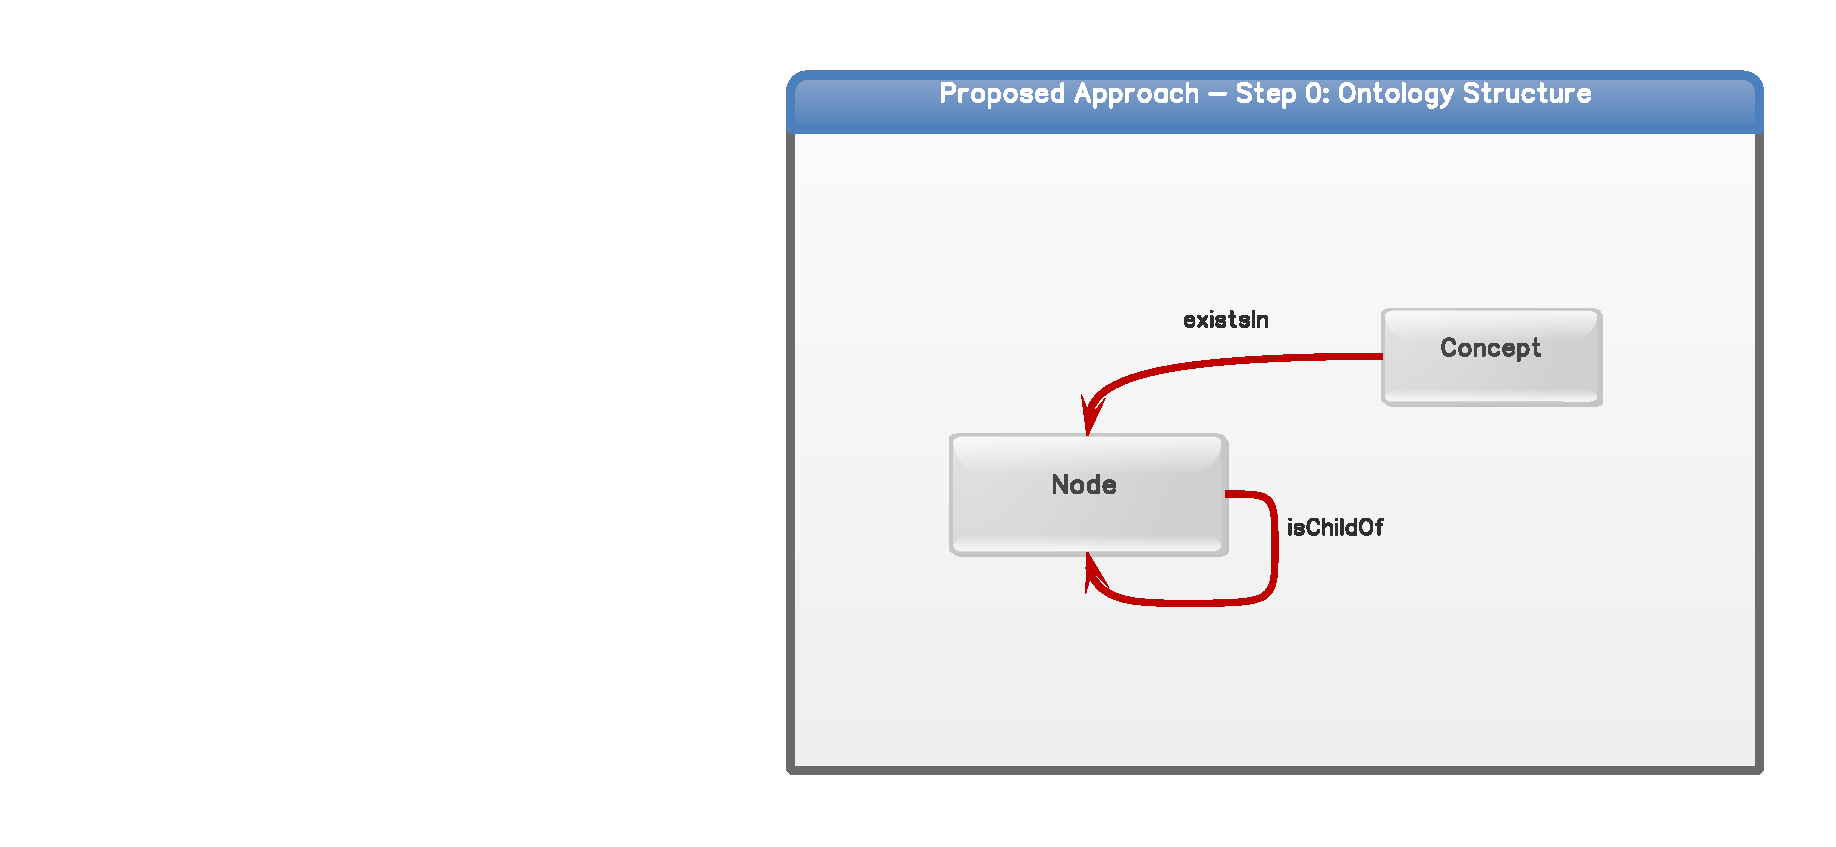
\includegraphics[scale=0.39]{graphics/c3/main_c3_0}
\end{frame}

\begin{frame}
	\frametitle{$C_{3}$: Proposed Approach - Knowledge Extraction}
	\begin{block}{}
	 \begin{itemize}
	  \item Clustering concept vectors using \alert{k-means},
	  \item Clustered conceps are populated within the ontology.
	 \end{itemize}
	\end{block}
	\hspace*{-1cm}\centering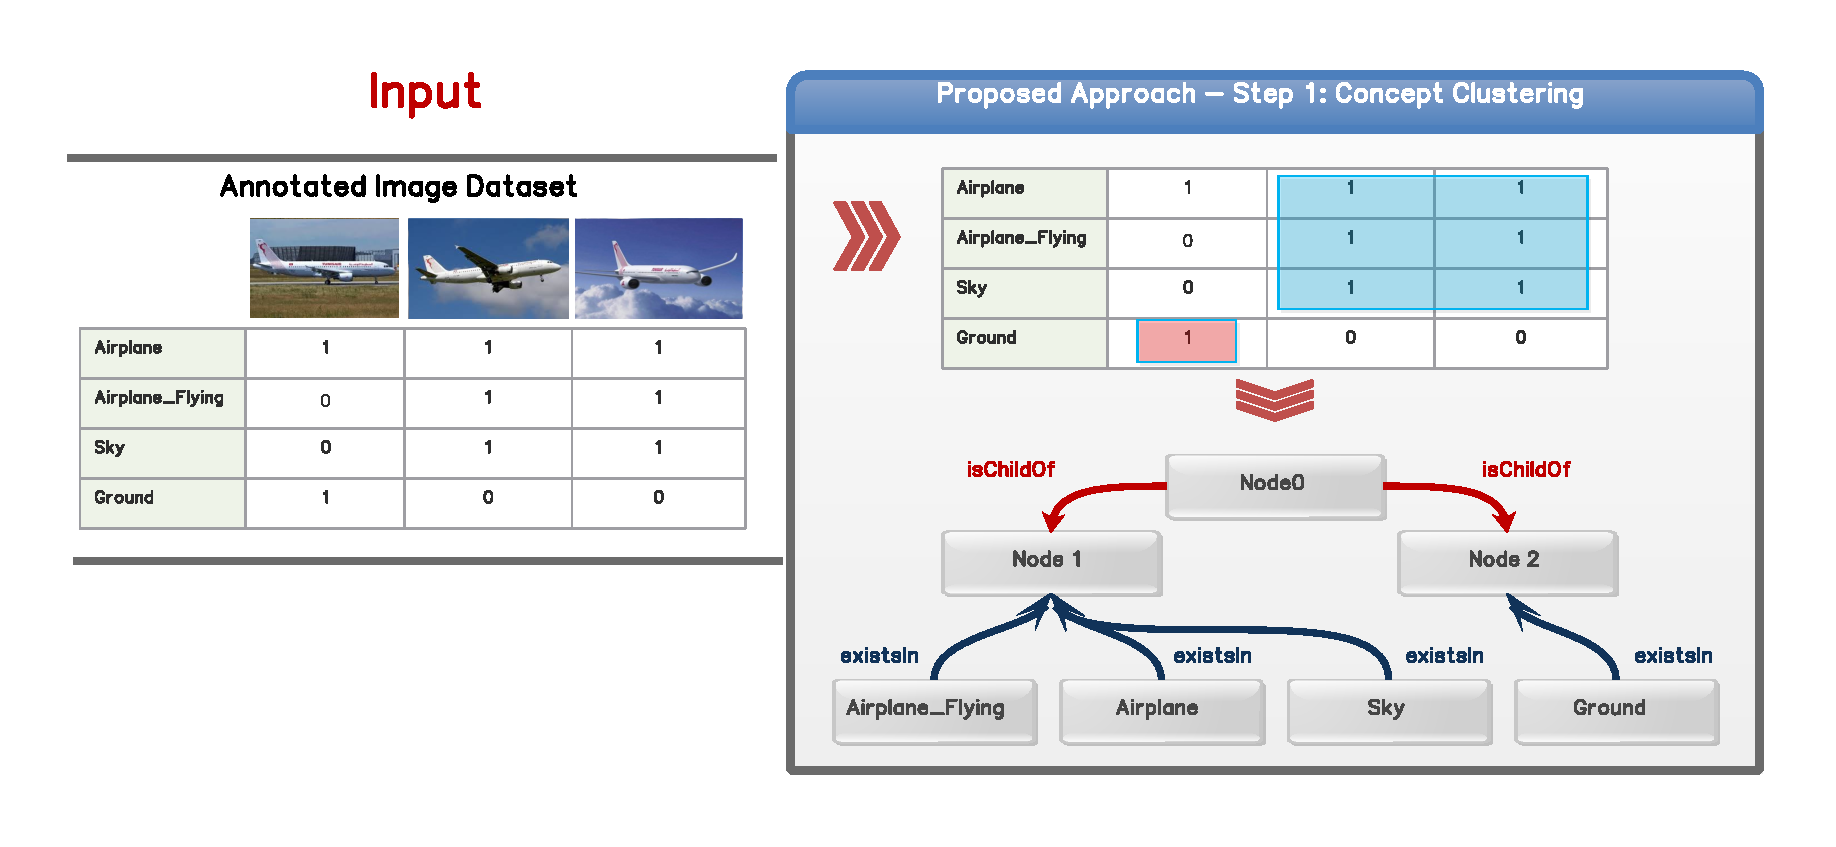
\includegraphics[scale=0.39]{graphics/c3/main_c3_2}
\end{frame}


\begin{frame}
	\frametitle{$C_{3}$: Hierarchical Semantic Detectors Construction}
	\begin{block}{}
	 \begin{itemize}
	  \item Extract \alert{\textsc{Sruf}} features from annotated images,
	  \item one-vs.-one linear kernel \alert{\textsc{Svm}} based learning algorithm.
	 \end{itemize}
	\end{block}
	\hspace*{-1cm}\centering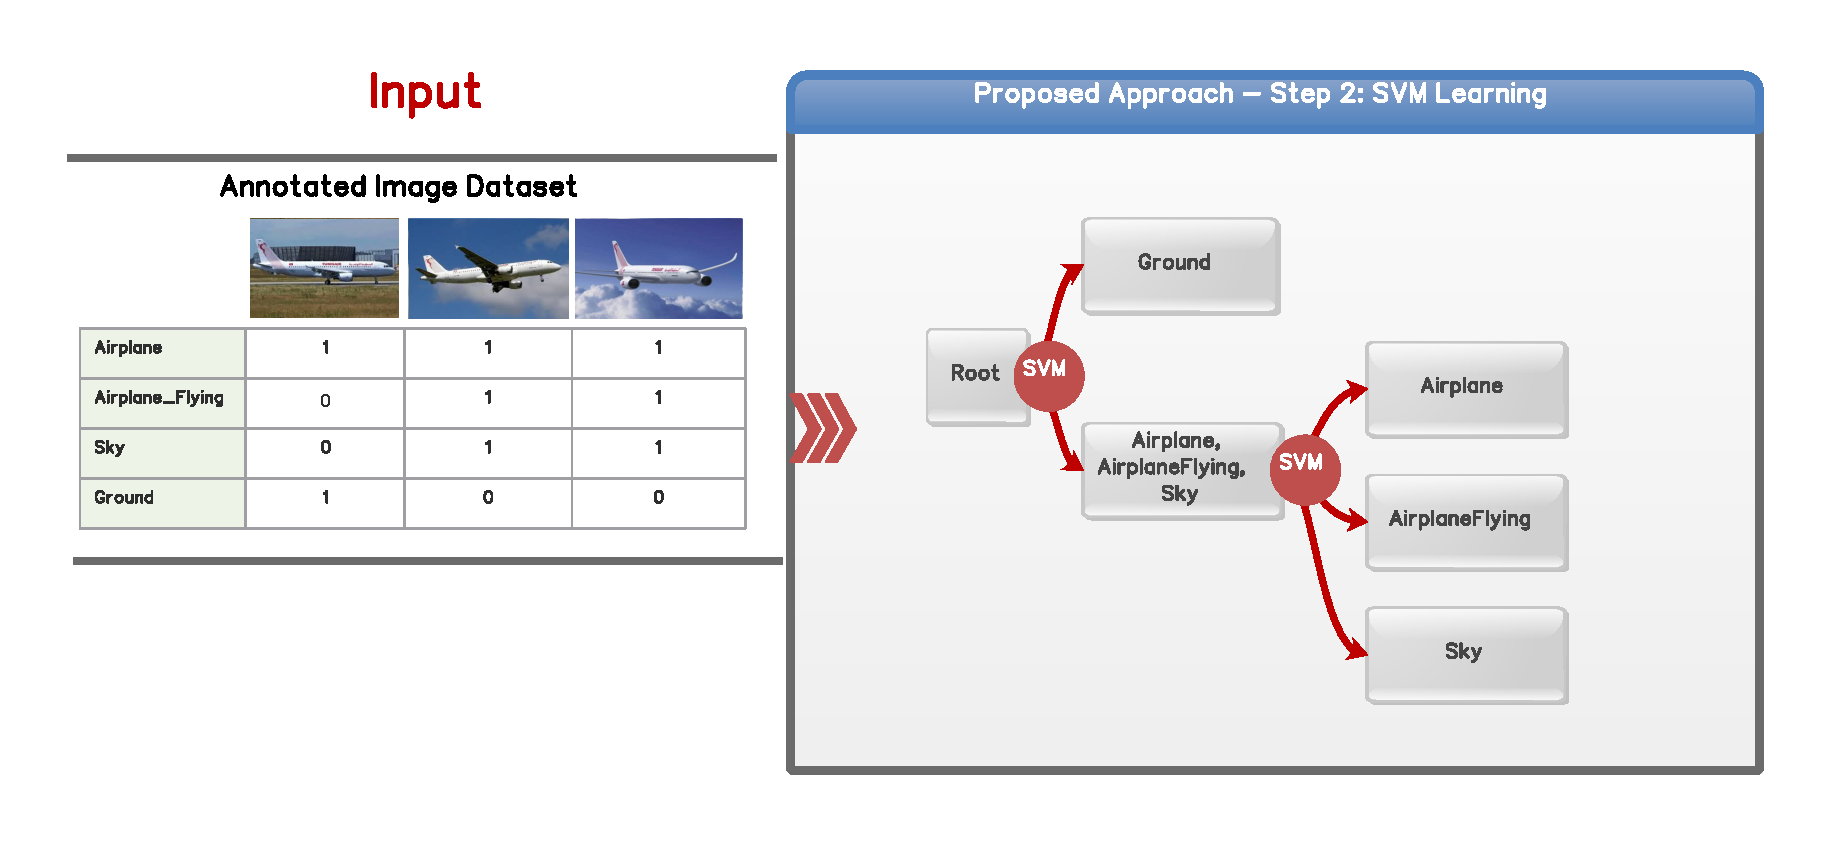
\includegraphics[scale=0.39]{graphics/c3/main_c3_3}
\end{frame}

\begin{frame}
	\frametitle{$C_{3}$: Hierarchical Semantic Image Annotation}
	\begin{block}{}
	 \begin{itemize}
	  \item \alert{Walking} the concepts hierarchy,
	  \item In each level, the \textsc{Svm} detects concepts to be \alert{excluded}.
	 \end{itemize}
	\end{block}
	\hspace*{-1cm}\centering\includegraphics[scale=0.39]{graphics/c3/main_c3_4}
\end{frame}

\begin{frame}
	\frametitle{$C_{2}$: Experiments - Setup}
	\begin{exampleblock}{Experimentation Setup}
		{\small
		\begin{itemize}		
			\item \textsc{ImageClef 2015}
			\item Photo dataset : \alert{\textbf{500.000}} images \\ (only \textbf{1.500} images were annotated)
			\item \alert{251} semantic concepts
		\end{itemize}
		}
	\end{exampleblock}
\end{frame}

\begin{frame}
	\frametitle{$C_{2}$: Experiments - Results}
	\begin{exampleblock}{Accuracy Evaluation}
		{\small
		\begin{itemize}		
			\item Only \alert{$300.000$} images were annotated.
		\end{itemize}
		%\begin{table}
		\centering
		\begin{tabular}{ l| l l }
				\hline
				\textbf{\small } 	& \textbf{\small MAP} &	 \\
				\hline \hline
				\textbf{\small Best run}  & {\small $0,659507$}		& {\small(/SMIVA/21.run)} \\
				\textbf{\small Worst run} & {\small $0,000231898$}	&  \\
				\textbf{\small Average}	  & {\small $0,18673$} 		&  \\
				\textbf{\small Our best run~~}& {\small$0,0161687$} 	&  {\small(position $75/89$)} \\
				\hline
				\end{tabular}
		%\end{table}		

		}
	\end{exampleblock}
	%\pause
	\begin{exampleblock}{Scalability Evaluation}
		{\small
		\begin{itemize}		
			\item An average \alert{$52$} \textsc{Svm} classifiers were fired ($min=6$ and $max=175$) 
				instead of firing all the \alert{$251$} \textsc{Svm} classifiers
			\item \alert{Reducing about $80\%$ the number of concept to be detected}
		\end{itemize}
		}
	\end{exampleblock}
\end{frame}

\begin{frame}
	\frametitle{$C_{3}$: Related publication}
	\begin{block}{}
		\begin{itemize}
			\item \citep{Zarka2015a} \textbf{Zarka, M.}, Ben Ammar, A., \&{} Alimi, A. (2015). 
				Regimvid at imageclef 2015 scalable concept image annotation 
				task: Ontology based hierarchical image annotation. 
				In \emph{Working notes for CLEF 2015 conference , 
				Toulouse, France, September 8--11, 2015.}
		\end{itemize}
	\end{block}	
\end{frame}


%%%%%%%%%%%%%%%%%%%%%%%%%%%%%%%%%%%%%%%%%%%%%%%%%%%%%%%%%%%%%%%%%%%%%%%%%%%%%%%%%%%%%%%%%%%%%%%%%
	\section{Conclusions and Future Research Directions}
		\subsection{Conclusions}
		\begin{frame}
	\frametitle{Conclusions}
	\begin{block}{}
	\begin{itemize}
		\item The use of fuzzy knowledge based approach for video semantic 
		interpretation enhancement is an interesting research direction,
		
		\item With the obtained results, we demonstrated that such an approach 
		could help to resolve main multimedia community issues: \alert{semantic gap}, 
		and \alert{scalability},
		
		\item Further works are required to address more these issues. 
		Fortunately, more interesting research directions could be touched on.
	\end{itemize}
	\end{block}
\end{frame}

			
		\subsection{Future Research Directions}
		\begin{frame}
	\frametitle{Future Research Directions}
	
	\begin{alertblock}{}
		\begin{itemize}
		\item \textbf{Ontology evolution} and \textbf{domain adaptation} should be more tackled 
 		{\tiny{\citep{Hoffman2014,Liu2016}}},
		
		\item \textbf{Video genre} could refine further the managed knowledge, 
		and then the semantic capabilities
 		{\tiny{\citep{Wu2012, Huang2012, Chattopadhyay2013, Muneesawang2014}}},
		
		\item \textbf{Deep Neural Networks} for more \alert{accuracy} and \alert{scalability}
		{\tiny{\citep{Wu2015,Druzhkov2016}}},
		
		\item \textbf{Semantic Deep Learning} to extract and manage valuable knowledge
		{\tiny{\citep{Wang2015SemanticDL}}}.
		\end{itemize}
	\end{alertblock}
\end{frame}

			

		\begin{frame}[allowframebreaks]
			\renewcommand*{\bibfont}{\tiny}
			\frametitle{Publications}
				\bibliographystyle{apalike}
    				\bibliography{bibliography/mybib2}
			\end{frame}
			

	\begin{frame}[plain]
  		\begin{center}\begin{huge}\textbf{\alert{Thank you for your attention}}\end{huge}\end{center}
	\end{frame}


\end{document}
